\ifgerman{\chapter{Evaluierung}}{\chapter{Evaluation}}
\label{evaluation}

This chapter contains the discussion of the evaluation methodology, which comprises of measures to determine how well different estimators perform, as well as the structure and results of our testing.

\section{Performance criteria}
\label{evaluation:objective}

The selection of measurements for comparison should be guided by what is expected of a performance estimator. Highest on the priority list is the requirement that its estimate $\widehat{acc_c}$ is equal or at least close to the true value $acc_c$. This criterion is actually bipartite: how large is the difference between the two on average and does it show a preference. The latter is commonly referred to as \textit{bias}, while in the following, the former will be called \textit{spread}. When comparing two estimators, the primary focus is on the bias; a low spread is not exactly useful when it is centered around a wrong value.

The estimation of bias and spread are done, based on measures used in \cite{FigueroaEtal2012}, by computing the \textit{mean error (ME)} and the \textit{mean squared error (MSE)}:
\begin{subequations}
\begin{equation}
ME(k) = \frac{1}{n} \sum_{X \in \mathcal{X}^k}^{} \left(acc_c(X,\mathcal{D}) - \widehat{acc}_c(X,\mathcal{D})\right)
\end{equation}
\begin{equation}
MSE(k) = \frac{1}{n} \sum_{X \in \mathcal{X}^k}^{} \left(acc_c(X,\mathcal{D}) - \widehat{acc}_c(X,\mathcal{D})\right)^2
\end{equation}
\end{subequations}
where $\mathcal{X}^k$ contains the different training sets $X$ used in testing of size $k$. Lower values for ME and MSE indicate a better estimator.

Depending on the method in question, additional measures for comparison may be available. As a side effect of the multiple functions fit when using path or path-superset sub-sampling, the resulting estimates can be seen as sample points. The mean and variance of them specify a probability distribution. Luckily, the choice of the distribution model to assume is fairly simple, as most models are not suitable anyway since they are defined on $\mathbb{R}$. Our estimates, however, are limited to $[0,1]$. Thus, only few distributions come to mind, one of which is the beta distribution, also being used for similar purposes by \cite{KremplEtAl2014}. It is dependent by two parameters, $a, b \in \mathbb{R}_{\le 0}$, with a density function defined as \cite{GuptaEtAl2004}
\begin{equation}
q_{a, b}(x) = \frac{x^{a-1}(1-x)^{b-1}}{\int_{0}^{1} u^{a-1}(1-u)^{b-1}du}.
\end{equation}
The parameters are computable from mean and variance via
\begin{equation}
\begin{split}
E[Q] &= \mu = \frac{a}{a+b} = \frac{1}{|\mathcal{X}^k|} \sum_{X \in \mathcal{X}^k}^{} \widehat{acc}_c(X, \mathcal{D}) \\
var[Q] &= s^2 = \frac{ab}{(a+b)^2(a+b+1)} = \frac{\sum_{X \in \mathcal{X}^k}^{} (\mu - \widehat{acc}_c(X, \mathcal{D}))^2}{|\mathcal{X}^k|-1}
\end{split}
\end{equation}
Solving for $a$ and $b$ results in
\begin{equation}
\begin{split}
a &= \frac{\mu^2(1-\mu)}{s^2} - \mu \\
b &= a\left(\frac{1}{\mu}-1\right)
\end{split}
\end{equation}
The function $q$ is then the \textit{probability distribution function (PDF)} of the estimated accuracy distribution of $\widehat{acc}_c$. Now, the measure to compare the estimated and the \textit{true} accuracy distribution denoted by $P$ is the \textit{Kullback-Leibler divergence (KLD)}:
\begin{equation}
KLD(P:Q) = \int_{}^{} p(x) \cdot log_2\left(\frac{p(x)}{q(x)}\right) d\lambda (x),
\end{equation}
$p(x)$ is the PDF of the distribution $P$ \cite{KullbackEtAl1951}. The KLD is an information-theoretical measure intended to compare two probability distributions. If the two are equal almost everywhere, it equals zero, otherwise returns a positive value. Importantly, it is neither symmetrical nor does it satisfy the triangular inequality, thus the choice of distribution assignment is meaningful and should be equal for all tested methods (i.e. the distributions Q must not be swapped) \cite{Joyce2011}. As the integral cannot be evaluated in closed form, numerical integration is used instead:
\begin{equation}
KLD(P:Q) = \frac{1}{|N|} \sum_{n \in N}^{} p(n) \cdot log_2\left(\frac{p(n)}{q(n)}\right)
\end{equation}
with $N = \{\frac{1}{10000},...,\frac{9999}{10000}$. Due to the lack of floating point precision in Octave, which was used to implement the framework, the edge cases 0 and 1 were omitted; the values there for $p$ and $q$ were mostly zero or NaN.

Another important aspect of an estimator is its time complexity: only marginal improvements in bias of an estimator compared to its peers are unlikely to compensate for a drastic increase in computation time. Thus, it is also regarded in \ref{evaluation:results}.

\section{Method selection}

The method described in section \ref{methods} is build as a three-step process: first, some sort of sub-sampling for the subsets is performed (whether this actually reduces the amount of subsets is irrelevant). Then, the performance for the selected subsets is estimated and grouped. Last, the function model of choice is used to fit a curve on the groups and the final performance estimate obtained by extrapolating the functions to the set size $k$ and averaging the results. Including the possibility of using fitting improvements like weighting and the no-information rate as well as different function models, a lot of modules for each stage are available. Unfortunately, I cannot test all combinations, as it is quite time consuming.

Of course, some of the stage modules are incompatible: when using capped sub-sampling, applying path grouping is not possible, as there are no paths. Likewise, when path sub-sampling has been chosen, only path grouping is viable. Also, pre-screening suggested that the usage of the no-information rate as zero-set-size estimate is not as effective as hoped. Causes seem to be both high variance, leading to worsened fitting with low amounts of sub-samples, as well as its expendability for larger sub-sample sizes, which grow with the size of the training set.

\begin{table}[h]
\centering
\begin{tabular}{c | C{10cm}}
Method name & Description\\
\hline
5-Fold CV & 5-Fold cross-validation\\
.632+ BS & .632+ bootstrapping with 50 bootstrap samples\\
\hline
path & Path sub-sampling with path grouping\\
pathSuper & Path-superset sub-sampling with path grouping\\
averaged & Capped sub-sampling with averaged grouping; cross-validation for estimation\\
averagedBS & Capped sub-sampling with averaged grouping; .632 bootstrap for estimation\\
\hline
pathW & path with statistical weighting for fitting\\
pathSuperW & pathSuper with statistical weighting for fitting\\
averagedW & averaged with statistical weighting for fitting\\
averagedBSW & averagedBS with statistical weighting for fitting\\
\hline
pathSuperNI & pathSuper with the no-information rate as estimate for subset size 0
\end{tabular}
\caption{Summary of all estimators evaluated in the tests}
\label{tab:allEstimators}
\end{table}

As a result of this, the testing is conducted for 11 different estimators: path and path-superset sub-sampling combined with path grouping, which will be abbreviated as \textbf{path} and \textbf{pathSuper}, as well as capped sub-sampling with averaged grouping with the name \textbf{averaged}. While the estimation technique for the two path-based methods will be exclusively cross-validation, \textit{averaging} is also tested with .632 bootstrapping with the identifier \textbf{averagedBS} to assess whether it has any impact on the quality of the methods. Additionally, each of these estimators are evaluated using both weighted and unweighted fitting, with the former being designated by a trailing \textit{W}. Additionally, to confirm the suspicions raised in our pre-screening, \textit{pathSuper} is also tested in a modified version with a 0th data point for each path/curve, named \textbf{pathSuperNI}. To complement the selection, the more traditional estimators 5-fold cross-validation and .632+ bootstrapping also participate as \textbf{5-fold CV} and \textbf{.632+ BS}. \ref{tab:allEstimators} lists all participating estimators and their description.

Additionally, each of these estimators is tested with the three potential function models explored in \ref{methods:function_models}: exponential, sigmoid, and linear model. Each graph's designation contains either \textit{"exp."}, \textit{"sig."} or \textit{"lin."} to indicate the model used.

\section{Test environment}

\subsection{Reference accuracy}

The ground truth $acc_c(X, \mathcal{D})$ is extracted with holdout testing. For this, all instances in $\mathcal{L}$ which are not part of $X$ are split in $m$ sets $H_i$ of size k; for the evaluation, $\mathcal{L} = \mathcal{D}$ since all instances are accompanied by a class label in the datasets used. Then, the accuracy of the classifier $x_X$ on each $H_i$ is computed. The holdout accuracy $acc_c$ then equals the average accuracy over all $H_i$: $acc_c(X, \mathcal{D}) = \frac{1}{m} \sum_{i=1}^{m} acc_c(X, H_i)$. The $acc_c(X, H_i)$ also are used as the sample points from which the true accuracy distribution $P$ is computed: $\mu = acc_c(X, \mathcal{D})$, $s^2 = \frac{1}{m-1} \sum_{i=1}^{m} (\mu - acc_c(X, H_i))^2$.

\subsection{Function fitting}

As neither the exponential nor the sigmoid function model are linearizable, the fitting used the Levenberg-Marquardt algorithm, which, amongst others, requires the specification of initial parameters. Also, as a preconceived image of a learning curve as monotone rising and limited to the interval $[0, 1]$ exists, providing constraints to fulfill these requirements is reasonable. This is trivial for the sigmoid function, as it was specifically designed to allow this kind of modification: $y_0$ and $S$, as representations of the y-intercept and the function's asymptote, are limited to $[0,1]$ with $y_0 \leq S$, and $m$ has to be in $\mathbb{R}_{\geq 0}$. For the other functions it is not as easy to find suitable bounds: while both have parameters directly affecting the y-intercept and slope, their asymptote for $x \mapsto \inf$ is either affected by two parameters or is not a constant (linear). Both would require polynomial equality constraints, which were not taken into account for this work. Thus, it is good to keep in mind that these functions might violate the learning curve constraints.

\subsection{Active learner}

All tests are conducted with three different active learners: random sampling, uncertainty sampling and PAL; which one is indicated in the graphics. For their functioning see \ref{background:AL}. Although it does not matter due to the dichotomous nature of the used datasets, uncertainty sampling uses the maximum entropy for instance selection.

\subsection{Classifier}
\label{evaluation:classifier}
The choice of an adequate classifier is mostly limited by the active learners and the datasets used in the evaluation. From the dataset side, it has to be able to accept continuous features. The output of class assignment probability is necessitated by PAL and uncertainty sampling. Also, PAL requires some sort of density estimation; to keep the comparability of both active learners up, a classifier making use of kernel density estimation (KDE) is reasonable. Considering this, Parzen window lends itself to be the classifier of choice. It is a non-parametric classifier directly build on KDE. The assumption is that the data is distributed according to some probability distribution; basic assumption is the normal distribution. Then, the kernel $K$, which in our case is the probability density function (but it does not have to be), is approximated at a given instance $\vec{x}$ using the following formula:
\begin{equation}
\label{equ:uniKDE}
\hat{f}_h(\vec{x}, X) = \frac{1}{h \cdot |X|} \sum_{\vec{x'} \in X}^{} K(\frac{\vec{x}-\vec{x'}}{h})
\end{equation}
As the training set, $X$ contains the already known instances and $h$ is the so-called bandwidth, a smoothing factor for the kernel \cite{SheatherEtAl1991}. It has to be estimated, which is usually done by applying a function called \textit{Silverman's rule of thumb}, which is dependent on $n$, the dimensionality of the data, its estimated standard deviation and some statistical properties of the kernel largely irrelevant to this work. The classifier used in the evaluation however simply assumed a standard deviation of 0.1 across all dimensions. If the data in question is multivariate, \ref{equ:uniKDE} has to be a bit modified; $K$ is then usually the product of the kernel for each dimension, same goes for the bandwidth \cite{Silverman1986}.

\begin{figure}[h]
	\centering
	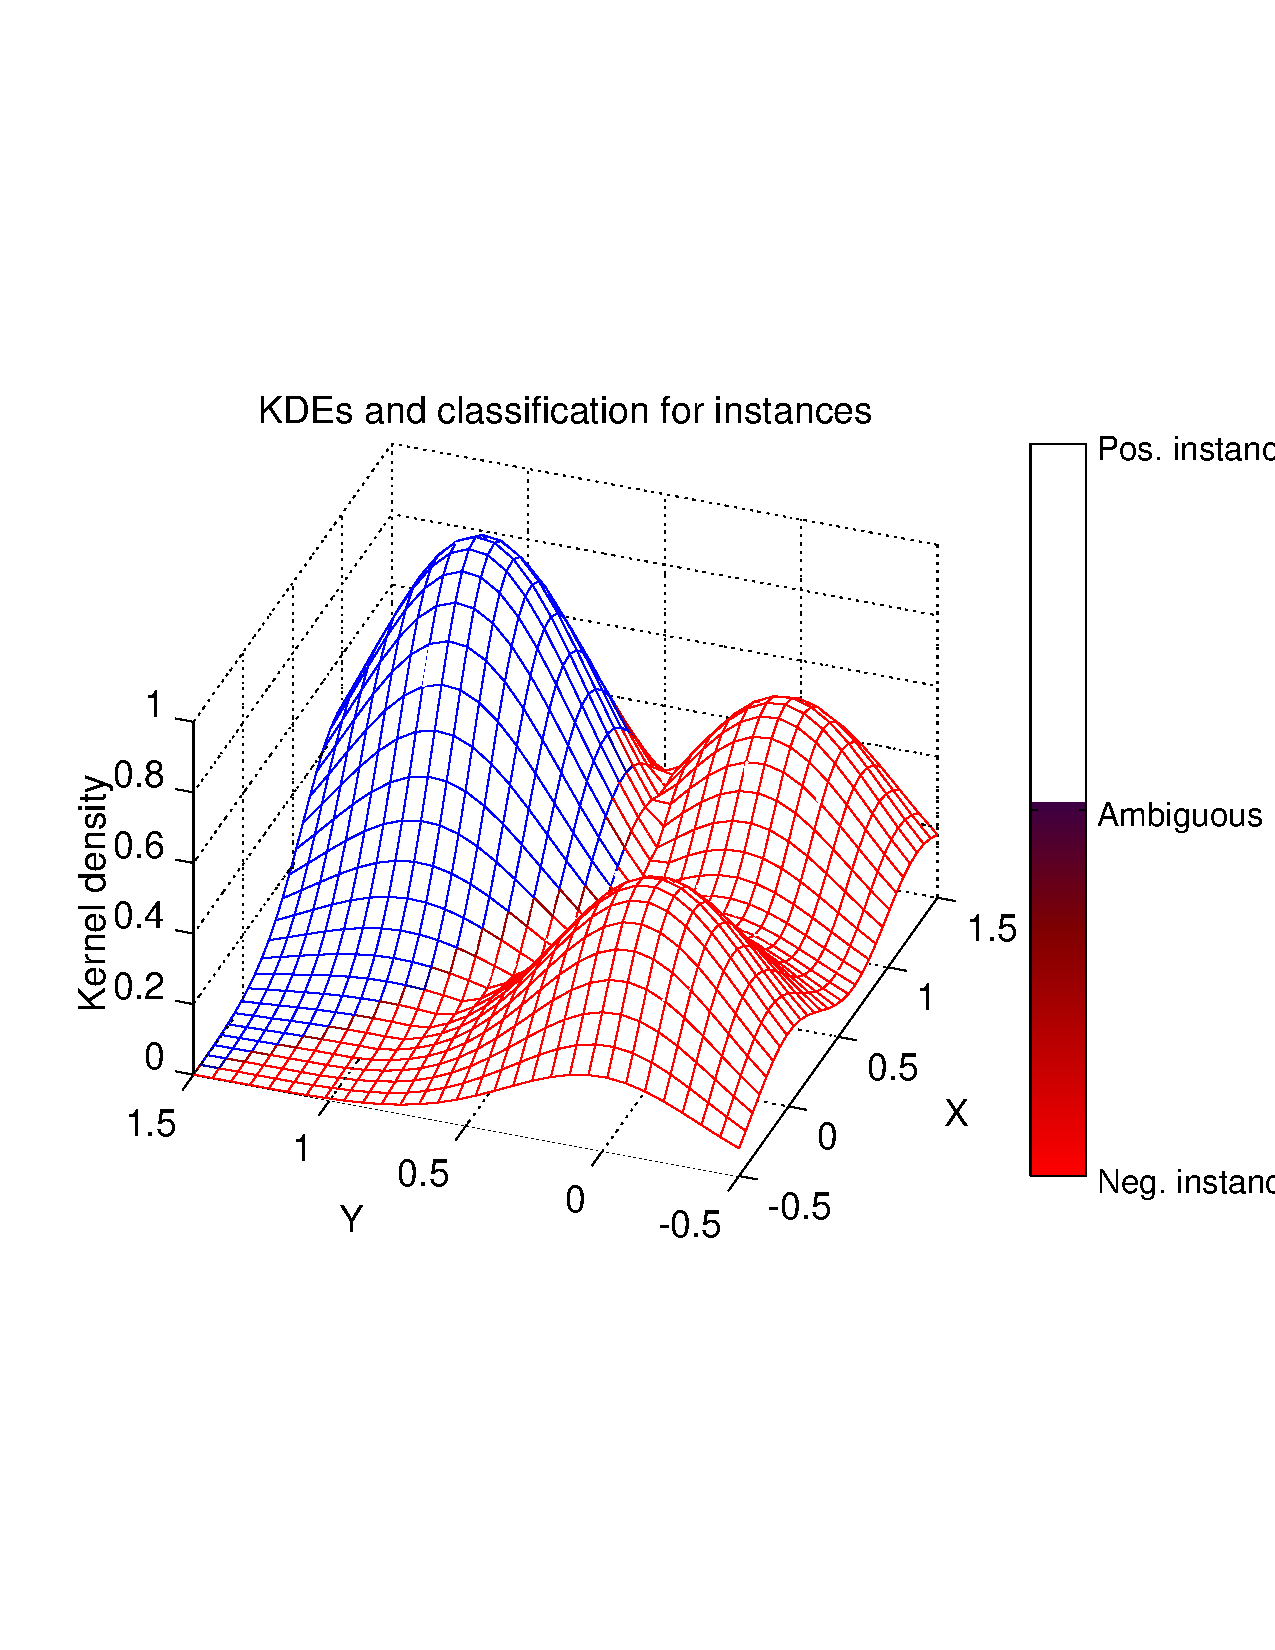
\includegraphics[trim = 0cm 6cm 0cm 5cm, clip = true, width = 0.8\textwidth]{KDE3inst}
	\caption{The estimated kernel density for a grid with one positive and two negative instances; lower Z value indicates lower certainty for the class assignment}
	\label{fig:KDE3inst}
\end{figure}

The Parzen window classifier estimates the densities of an instance to be labeled for each class label, each time using only the instances with the same label as $\vec{x}$. Then, they are multiplied with the prior class probabilities, i.e. the share each class label has among the labeled instances. Normalization then results in the wanted (estimated) class probabilities, with the largest probability dictating the resulting class \cite{ArchambeauEtAl2006}. \ref{fig:KDE3inst} shows the classification of a Parzen window classifier: the color expresses the predicted class label, while the z coordinate equals the kernel density with either one positive or two negative instances as its base, depending on which one is larger.

\subsection{Datasets}

The datasets used should both be realistic and cover most uses; a method that does well on specifically designed test sets but fails in the real world is only interesting as a proof-of-concept. Secondly, PAL was only defined for dichotomous data. Although an extension on multiple-class problems should be possible, I did not want to tamper with the formulas, instead restricting the datasets to binary-class problems.

Considering these constraints the selection contains the following datasets:

\begin{itemize}
	\item \textbf{checke1}: This artificial dataset was used in \cite{Chapelle2005} to examine active learning with Parzen window classifiers and contains 400 instances with two features. It has the form of a 4x4 checkerboard, with only every second field containing instances. There is no overlapping of class labels, i.e. the instances can be perfectly separated by class label using decision boundaries. This set may be problematic for uncertainty sampling as it will select instances at its decision boundary, while the set requires \textit{multiple} decision boundaries. Thus, it likely will not label instances from the other fields until it runs out of close ones. Both random sampling and PAL should not have this problem; the former does not care about any structure anyway, while the latter actively explores the "uncharted" instances.
	\item \textbf{2dData}: Also an artificial, 2-dimensional dataset, it was used in a follow-up paper on optimized PAL \cite{KremplEtAl2015} under the name "Sim". The 1200 instances are grouped into two clusters of roughly ellipsoid shape, but cannot be perfectly separated as they slightly overlap, making it seem more realistic (real-world datasets tend to have some noisy data). None of the active learners should have inherent problems with this set.
	\item \textbf{seeds}: A real-world dataset used in \cite{CharytanowiczEtAl2010}. It has seven features which describe different properties of wheat, classifying it into three varieties: Rosa, Kama and Canadian with 70 instances each. To comply with the constraints set earlier, the varieties Kama and Canadian were merged into one class. As it is 7-dimensional, obtaining a visual is difficult; thus "t-Distributed Stochastic Neighbor Embedding (t-SNE)", a method for dimensionality reduction of high-dimensional data \cite{vanDerMaaten2008} to project it into $\mathbb{R}^2$ by using Gauss kernels to keep neighboring instances together, rendered the visualization. Similar to \textit{2dData}, two clusters seem to be present, each containing instances sharing the same class label, albeit a small overlap exists. Due to the similarity, no problems regarding the active learners are to be expected.
	\item \textbf{abalone}: A real-world dataset using eight features associated with predict the age of abalones. Originally, the number of rings (and thus ages) of a specimen were predicted. To create a binary set, all ages below 10 form one class, while the rest forms the other. The set was obtained in the study \cite{NashEtAl1994}. As the original set contained 4177 instances, it had to be reduced to remain a viable option, considering the finite amount of time available for testing. Thus, the number of instances was reduced to 1800, keeping the class ratio intact. The visualization indicates the presence of four separate clusters with partially mixed class labels. While this may hint at problems with uncertainty sampling, the study itself suggests that the predictors are not sufficient for classification, leading to high error rates even with large training sets.
\end{itemize}

\begin{figure}[h]
	\centering
	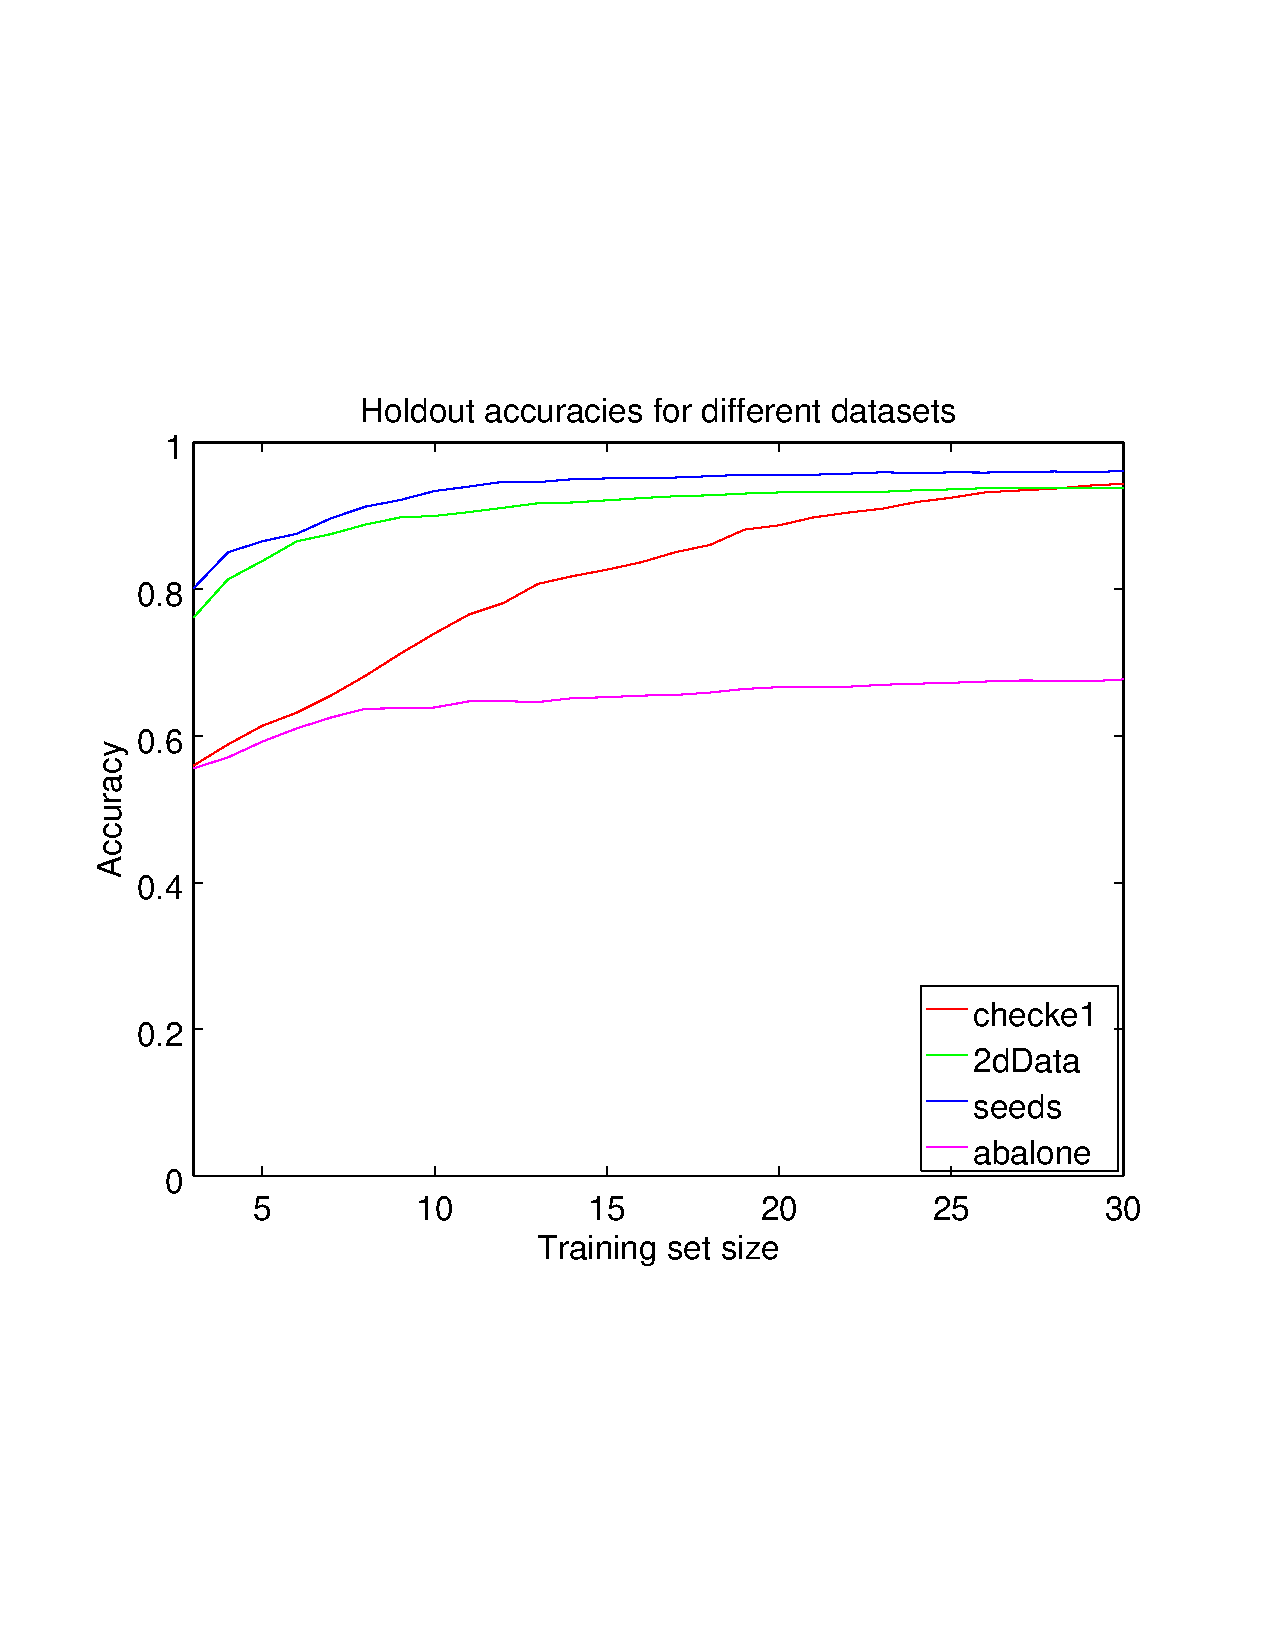
\includegraphics[trim = 1cm 6cm 2cm 6cm, clip = true, width = 0.6\textwidth]{holdoutAccs}
	\caption{Visualizations of the datasets checke1, 2dData, seeds and a downsized version of abalone \cite{Chapelle2005,KremplEtAl2014,CharytanowiczEtAl2010,NashEtAl1994}.\newline The illustration of seeds and abalone was done using an implementation of t-SNE \cite{vanDerMaaten2008}}
	\label{fig:holdoutAccs}
\end{figure}

\begin{figure}[h]
	\centering
	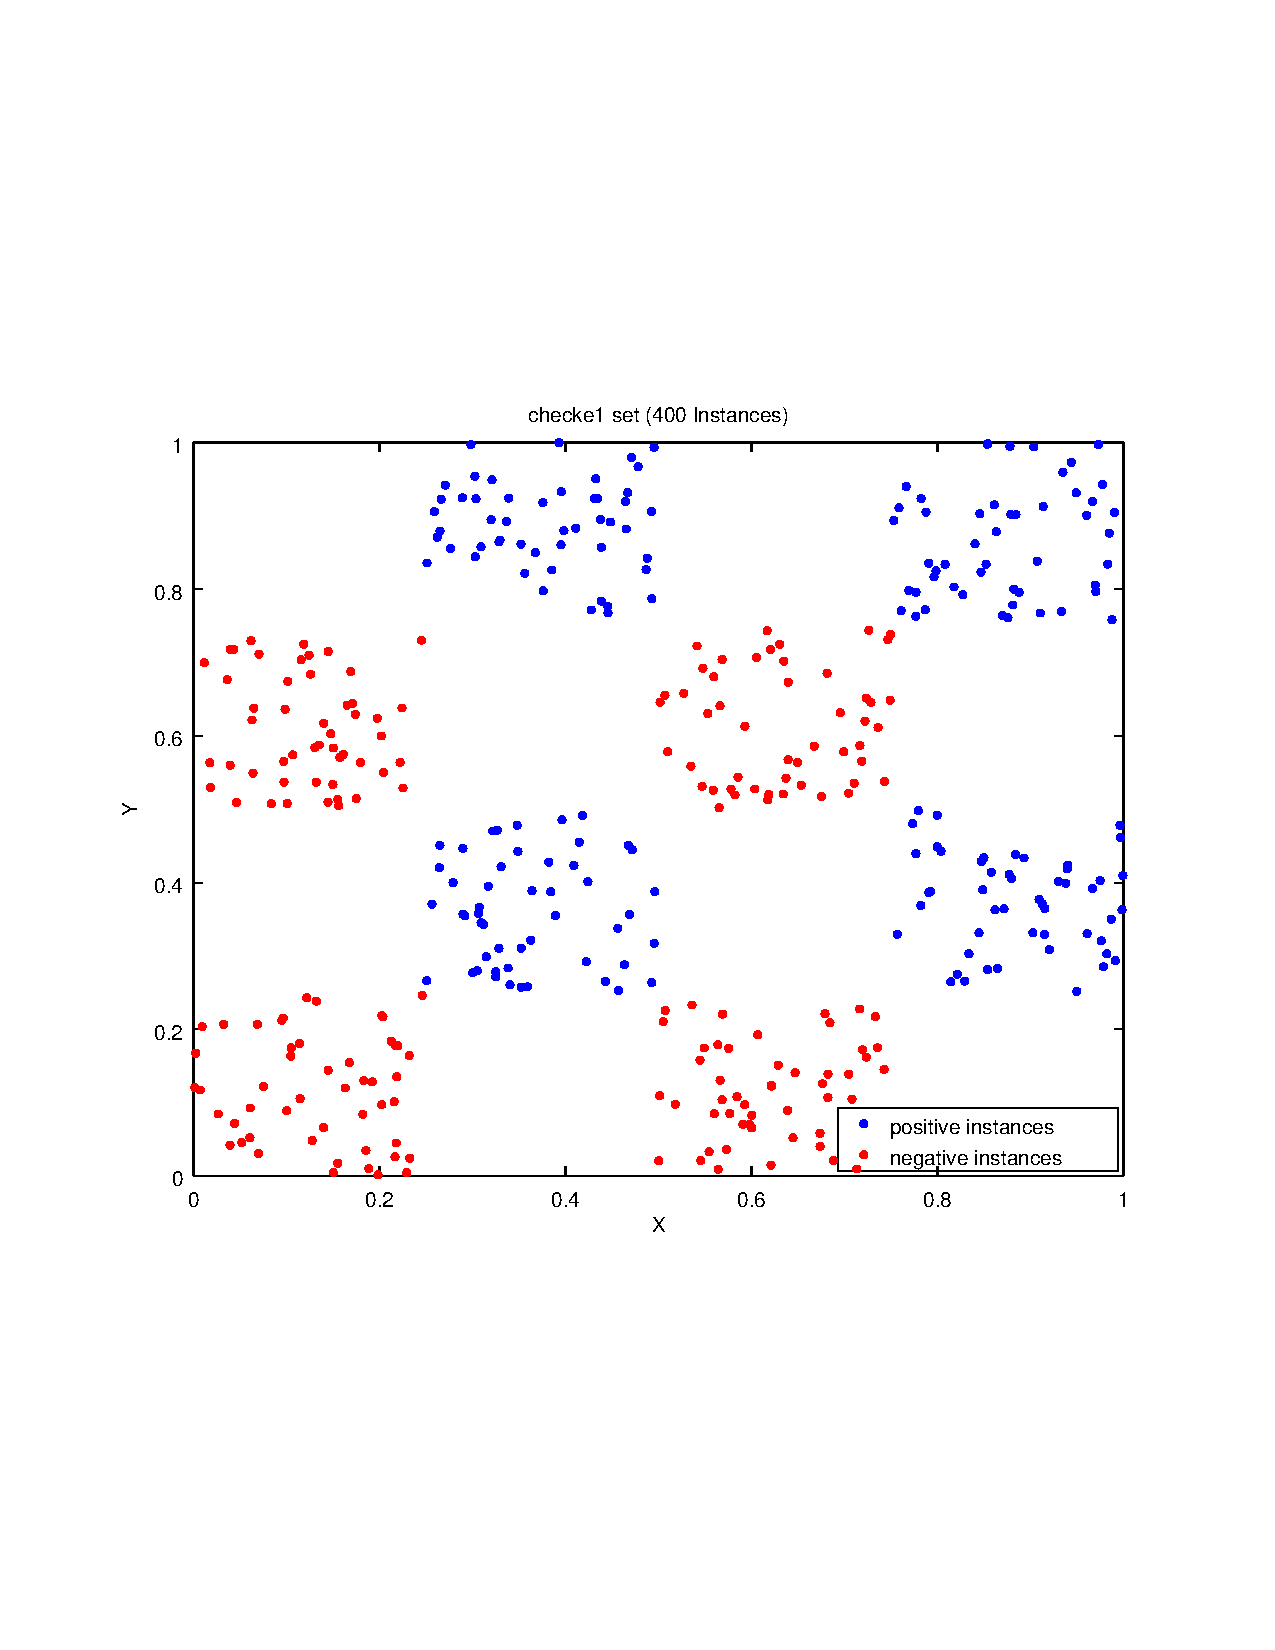
\includegraphics[trim = 1cm 6cm 2cm 6cm, clip = true, width = 0.45\textwidth]{checke1Illustration}
	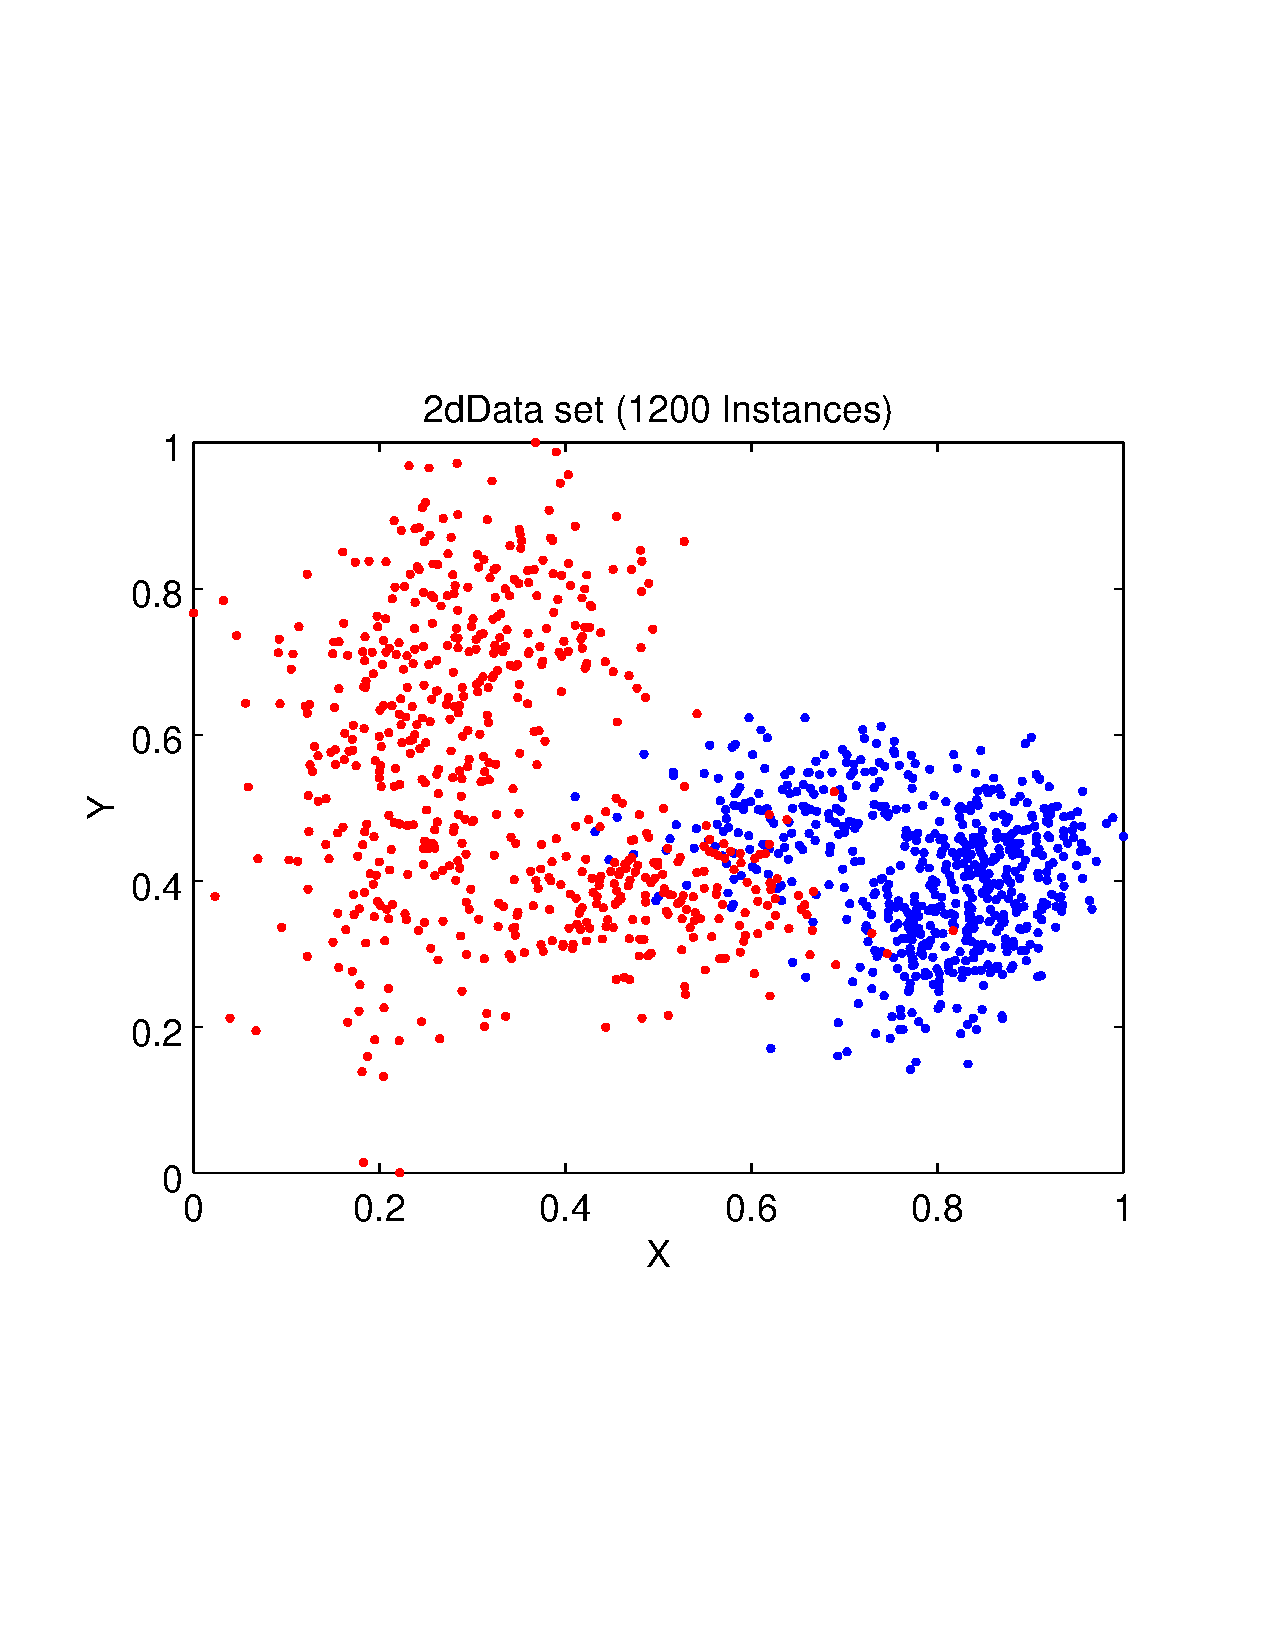
\includegraphics[trim = 1cm 6cm 2cm 6cm, clip = true, width = 0.45\textwidth]{2dDataIllustration}
	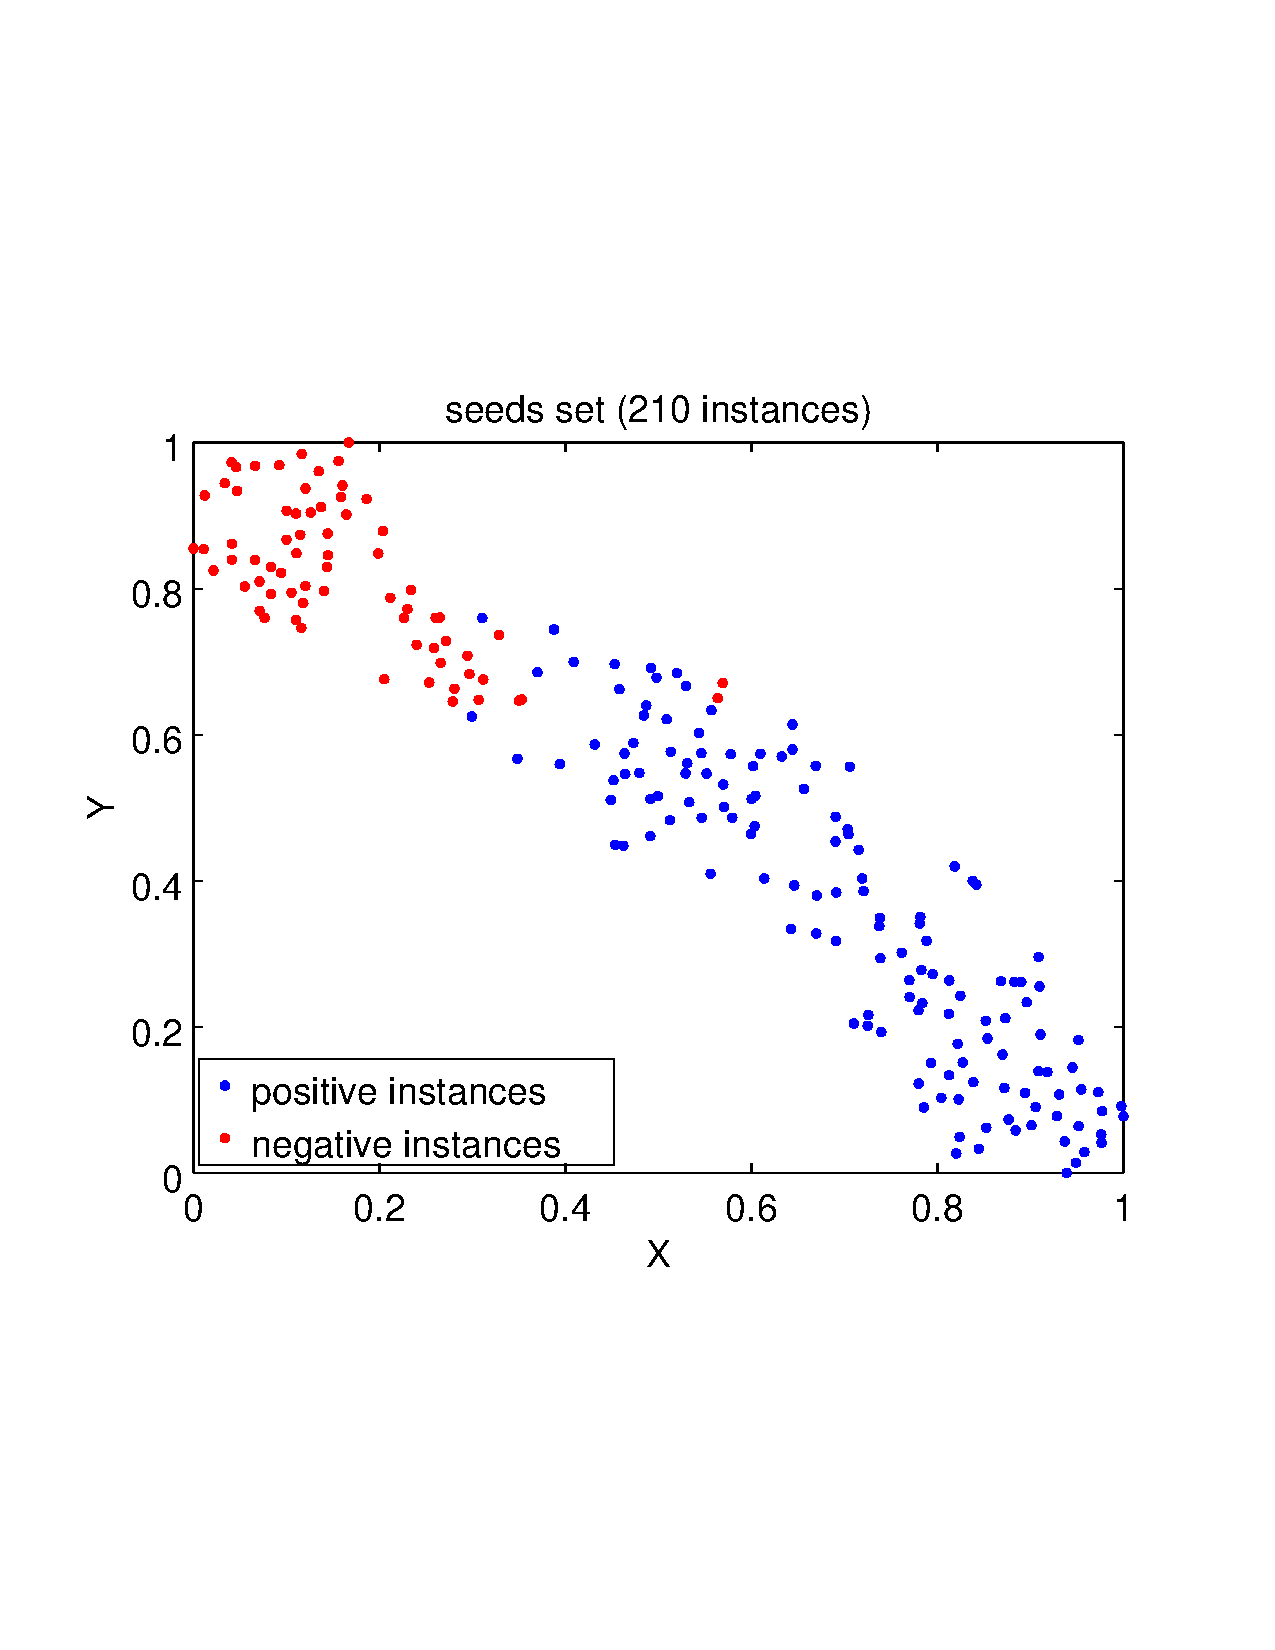
\includegraphics[trim = 0cm 6cm 2cm 6cm, clip = true, width = 0.475\textwidth]{seedsIllustration}
	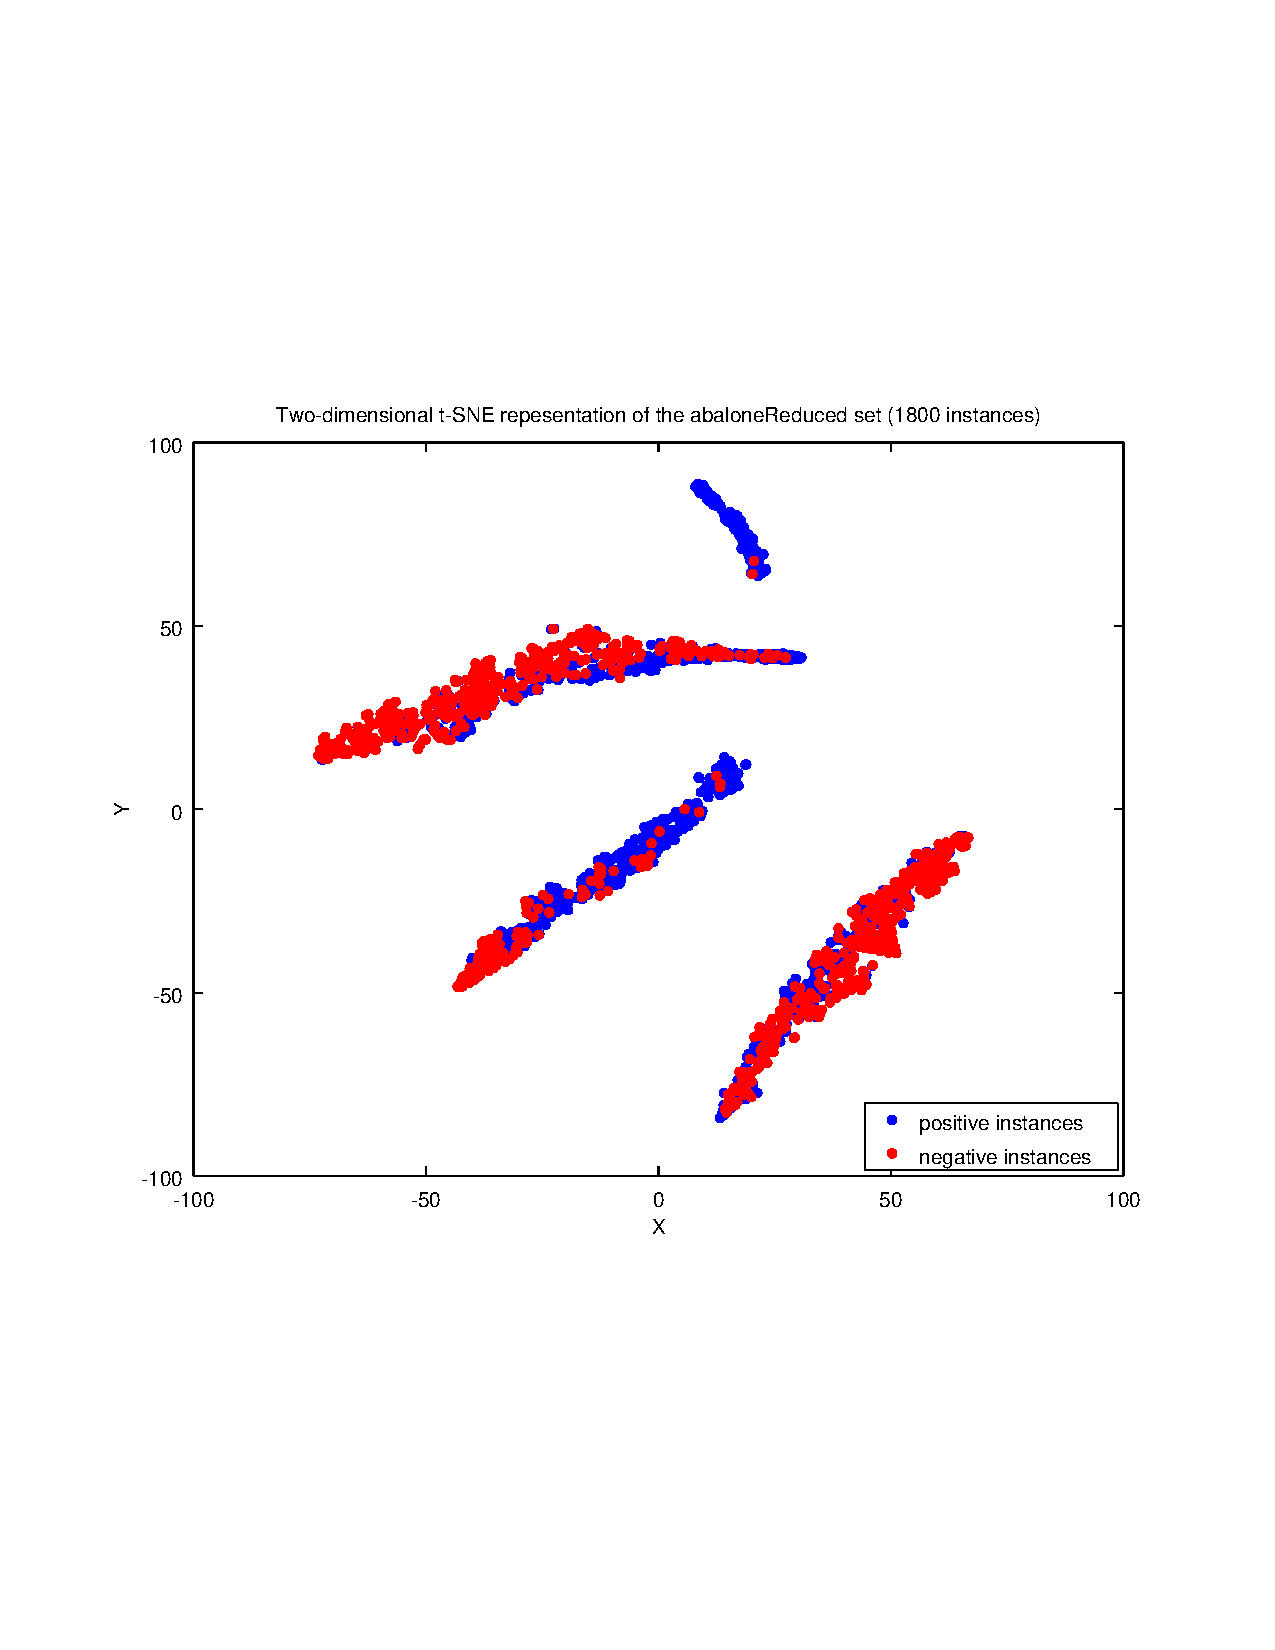
\includegraphics[trim = 1cm 6.6cm 2cm 6cm, clip = true, width = 0.475\textwidth]{abaloneReducedIllustration}
	\caption{Visualizations of the datasets checke1, 2dData, seeds and a downsized version of abalone \cite{Chapelle2005,KremplEtAl2014,CharytanowiczEtAl2010,NashEtAl1994}.\newline The illustration of seeds and abalone was done using an implementation of t-SNE \cite{vanDerMaaten2008}}
	\label{fig:datasetIllustrations}
\end{figure}

\ref{fig:datasetIllustrations} shows the two-dimensional visualization, while \ref{fig:holdoutAccs} illustrates the rough learning curve of a Parzen window classifier with random sampling of each dataset.

\subsection{Parameters}

Some of the methods as well as the fitting requires the specification of parameters like the number of iterations or error tolerance. As their choice may influence the results, all parameters used will be stated in this section.

For each combination of dataset, active learner and function model, 100 runs were simulated, each purchasing one instance at a time up to 30 and making estimates each step. All function models were fit on the same data.

For the \textit{path} and \textit{pathSuper} estimators, $k^2$ but not more than $\frac{10000}{k}$ paths were randomly selected. \textit{Averaged} makes use of all subsets up to ~10000 (due to rounding may not be exact); its bootstrap variant \textit{averagedBS} is allowed up to 50 subsets as well as 50 bootstrap samples per subset. Both caps were placed due to memory and time limitations. The modified variants with weighting/no-information rate use the same subsets/paths for any given test run. \textit{5-fold CV} has no limitations in place; \textit{.632 BS}, similarly to \textit{averagedBS}, also uses 50 bootstrap samples per estimation.

All functions were fit with the Levenberg-Marquardt algorithm, even the linear model; this was done to normalize the testing environment. The ranges for initial parameters as well as their bounds can be seen in \ref{tab:functionParams}. Each fitting can use up to 300 iterations with a scalar tolerance of $10^{-4}$, i.e. if the sum of squared errors is lower than $0.0001$, the fitting is considered done and will not use the remaining iterations. The partial derivatives were provided, thus numeric derivation was not necessary.

\begin{table}[h]
	\small
	\begin{tabular}{c | c | c | c}
	\textbf{Function model} & \textbf{Equation} & \textbf{Parameter bounds} & \textbf{Initial parameters} \\
	\hline
	3-Exponential & $f_E(x) = a + b \cdot e^{c \cdot x}$ & \begin{tabular}{l}$a \in [0,1]$ \\ $b \in [-\infty, 0]$ \\ $c \in [-\infty, 0]$\end{tabular} & \begin{tabular}{l}$a \in [0,1]$ \\ $b \in [-2, 0]$ \\ $c \in [-2, 0]$\end{tabular} \\
	\hline
	Sigmoid & $f_S(x) = a + b \cdot e^{c \cdot x}$ & \begin{tabular}{l}$a \in [0,1]$ \\ $b \in [-\infty, 0]$ \\ $c \in [-\infty, 0]$\end{tabular} & \begin{tabular}{l}$a \in [0,1]$ \\ $b \in [-2, 0]$ \\ $c \in [-2, 0]$\end{tabular} \\
	\hline
	Linear & $f_L(x) = a + b \cdot x$ & \begin{tabular}{l}$a \in [0,1]$ \\ $b \in [0, \infty]$\end{tabular} & \begin{tabular}{l}$a \in [0,1]$ \\ $b \in [0, 4]$\end{tabular} \\
	\end{tabular}
	\caption{Function-specific parameters for model fitting}
	\label{tab:functionParams}
\end{table}

As Levenberg-Marquardt may be stuck in local minima or not converge at all, each fitting was done 5 times with random parameters drawn from their respective ranges to attempt to circumvent these hazards. Then, the fit with the lowest sum of squared errors w.r.t. the data given was selected. If the fitting used statistical weights, they were also used in this selection.

\section{Test results}
\label{evaluation:results}
Due to the sheer amount of data, this section contains only the most expressive graphs. To help keeping an overview, the evaluation is structured into the following parts: first, we take a look at the mean error for the traditional and unweighted estimators using the exponential function model. After that follows a survey on whether the different models for fitting improve the bias or not, as well as what influence statistical weighting has. Then comes the comparison of the mean squared error for some selected estimators as well as the Kullback-Leibler divergence, for those it is available for. An analysis of the computation time necessary for each method finalizes the evaluation.

\subsection{Average Estimation Bias}

The evaluation results for the estimation bias is split into three figures. Each is comprised of four graphs, containing the mean estimation bias for the first six estimators of \ref{tab:allEstimators} used with the stated active learner and dataset. They are furthermore split into three adjacent bars, visualizing the bias of the estimator with training sets of the size $3 - 7$, $8 - 15$ and $16 - 30$, respectively. This is indicated by the darkened color for the larger set estimates. \ref{fig:meanErrorsExp} shows the results for estimators (except \textit{5-Fold CV} and\textit{.632+ BS}, as they do not utilize function model fitting) using the exponential model, while for \ref{fig:meanErrorsSig} and \ref{fig:meanErrorsLin} the sigmoid and linear ones have been used.

\begin{figure}[h]
	\centering
	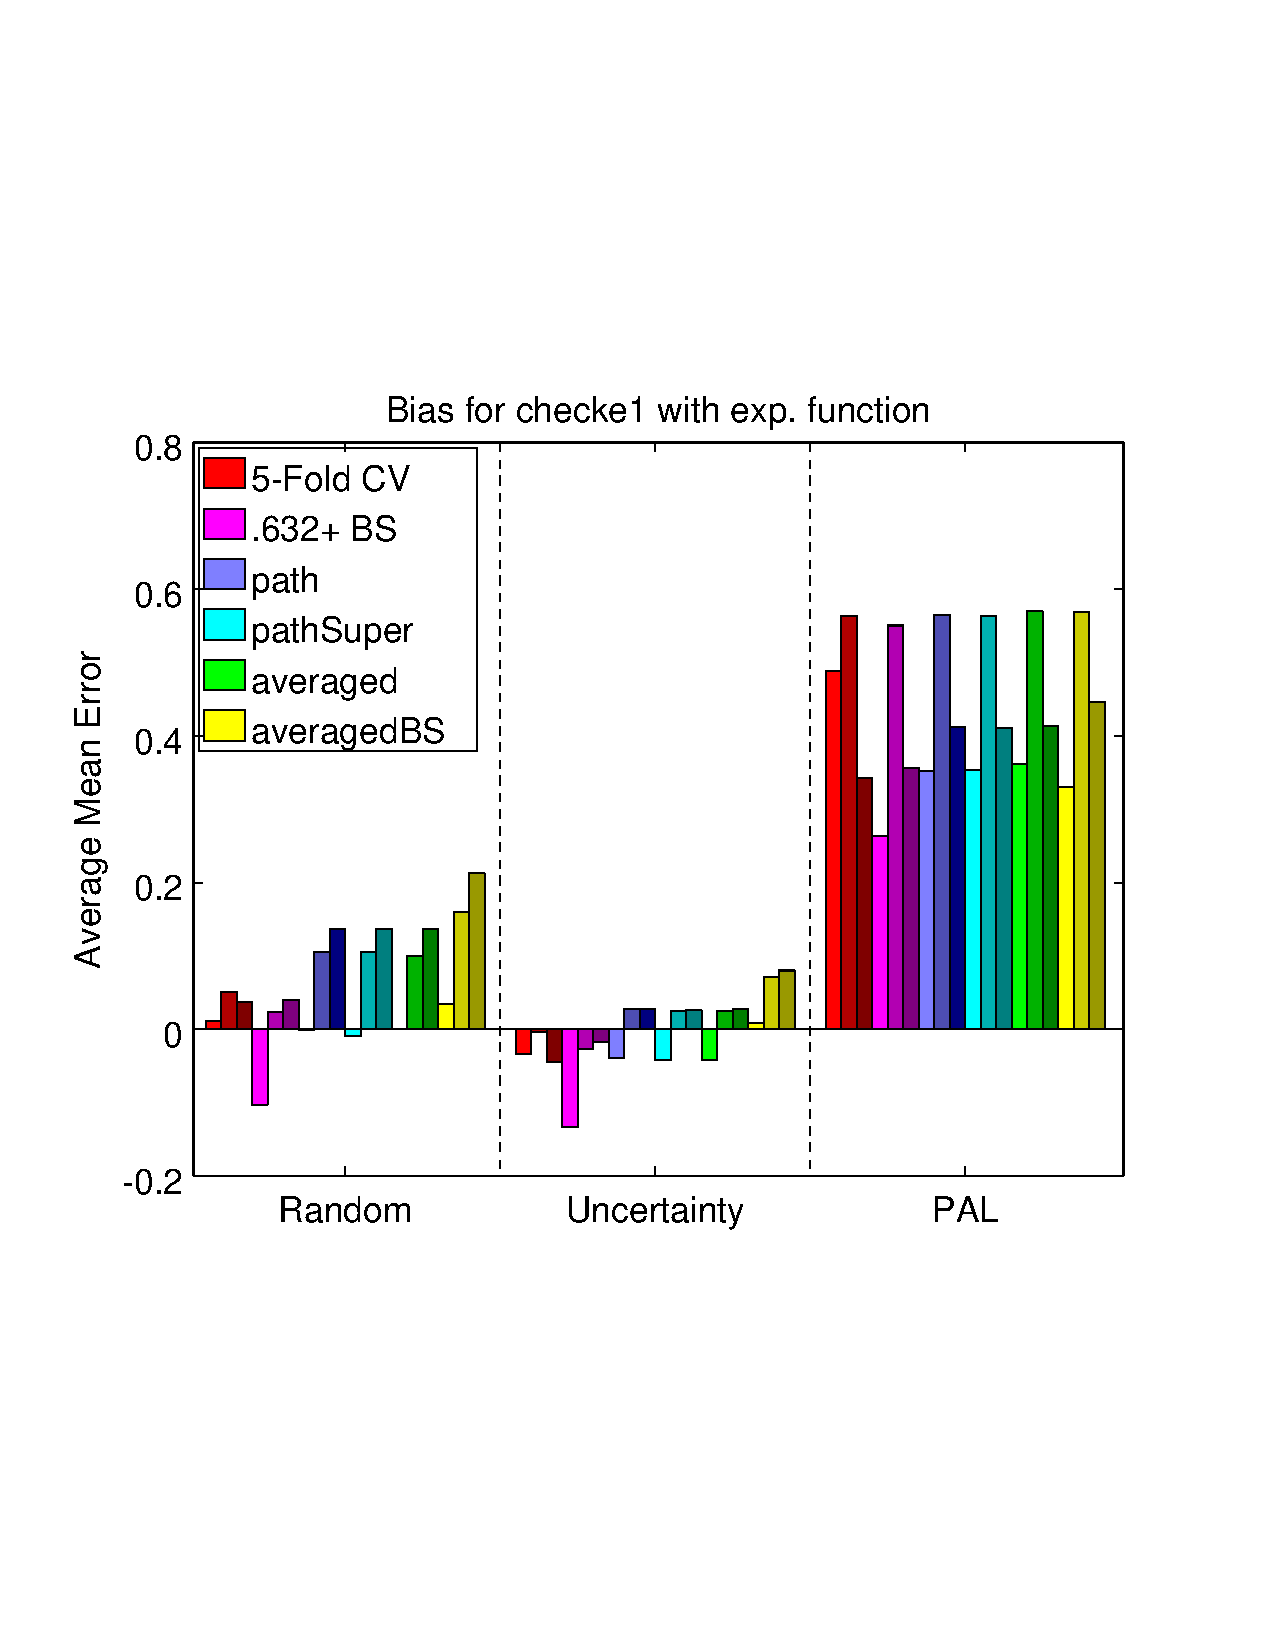
\includegraphics[trim = 1cm 6.5cm 2.5cm 6.5cm, clip = true, width = 0.48\textwidth]{meanErrExpchecke1}
	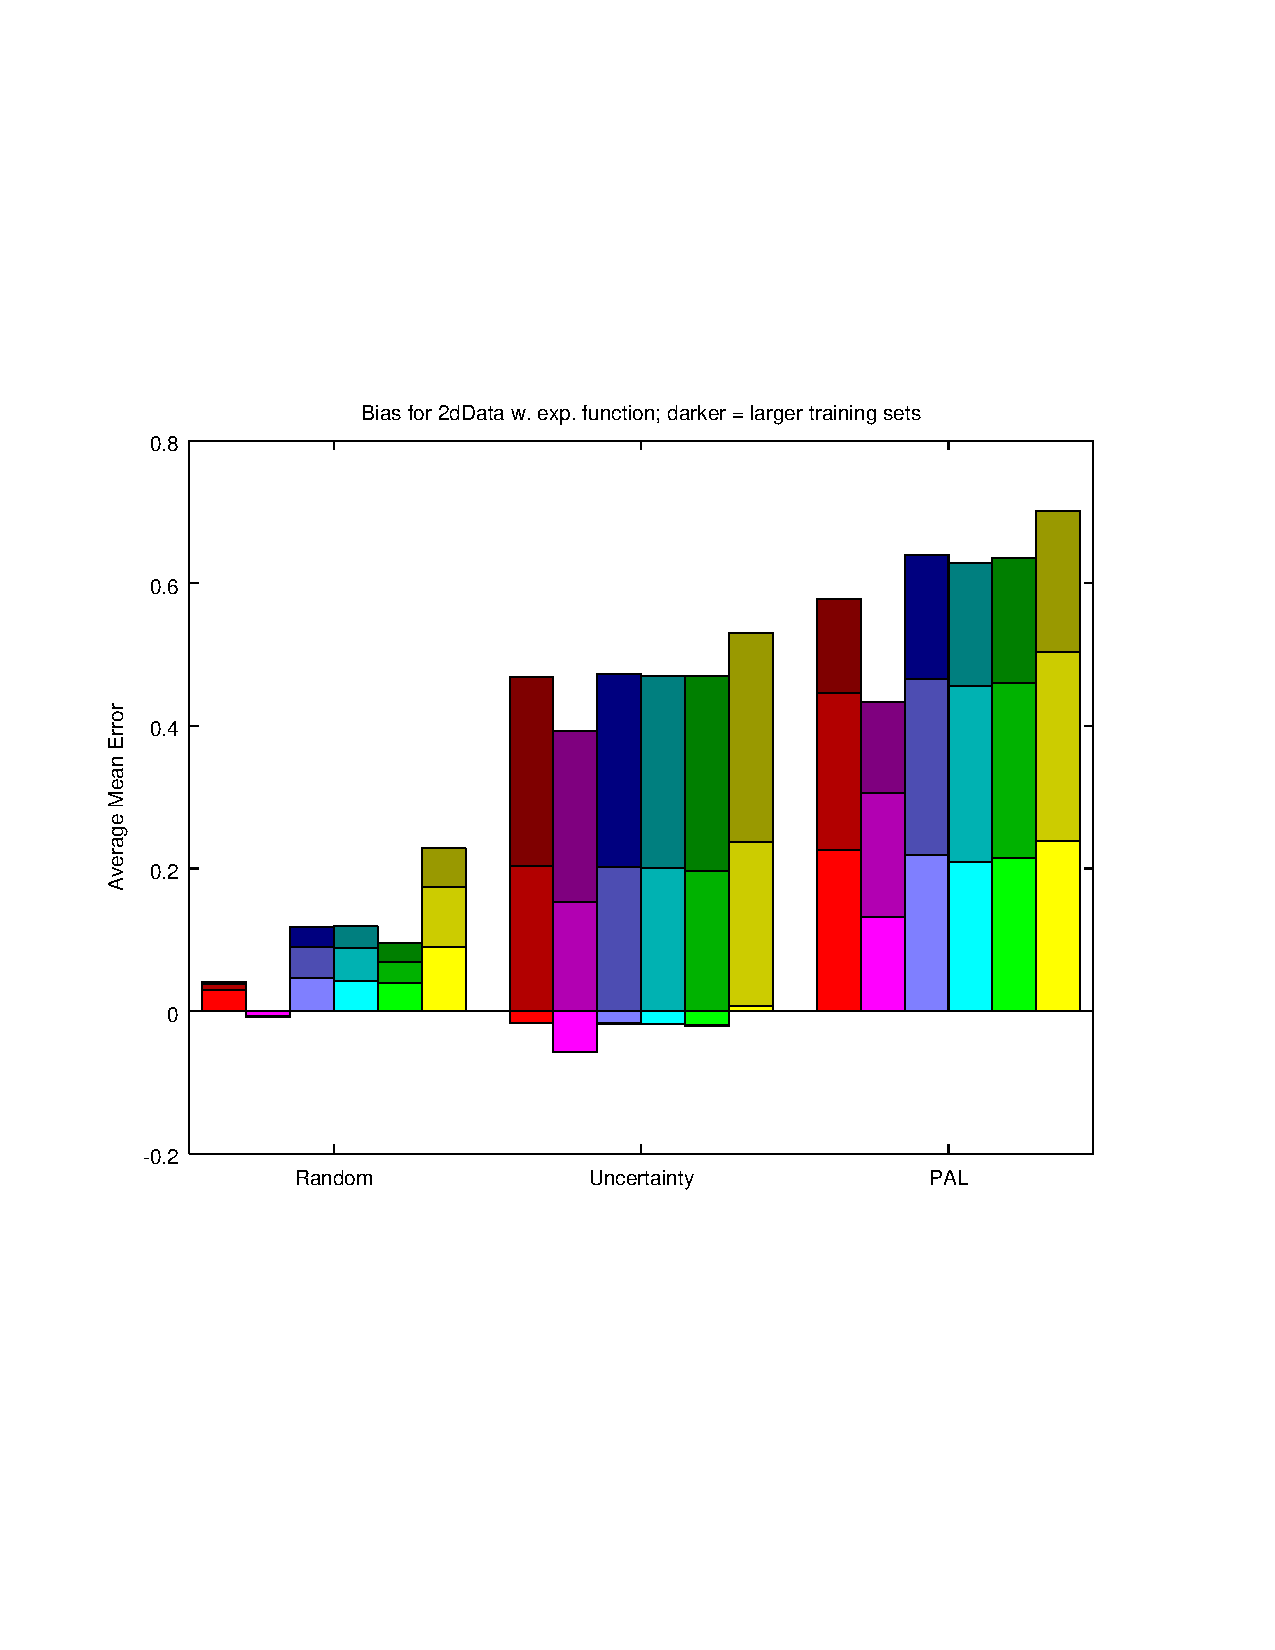
\includegraphics[trim = 1cm 6.5cm 2.5cm 6.5cm, clip = true, width = 0.48\textwidth]{meanErrExp2dData}
	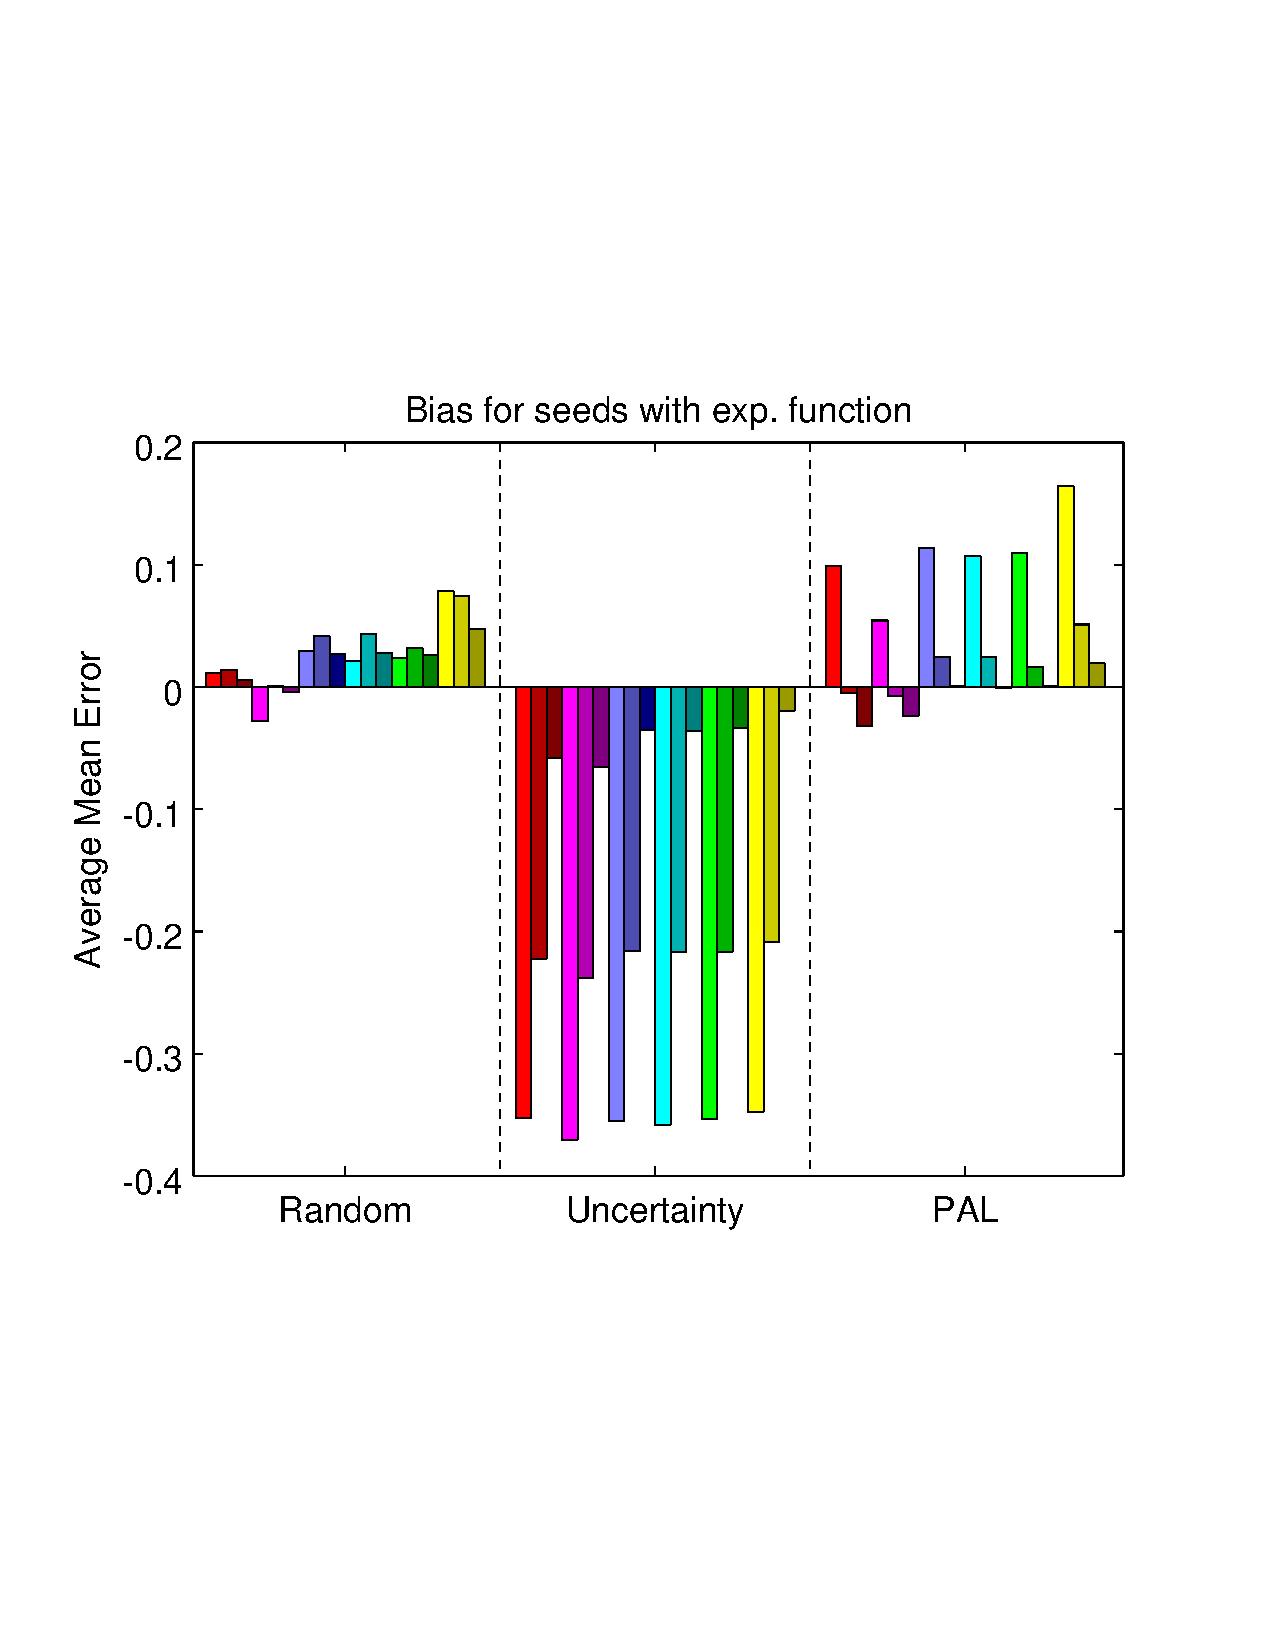
\includegraphics[trim = 1cm 6.5cm 2.5cm 6.5cm, clip = true, width = 0.48\textwidth]{meanErrExpseeds}
	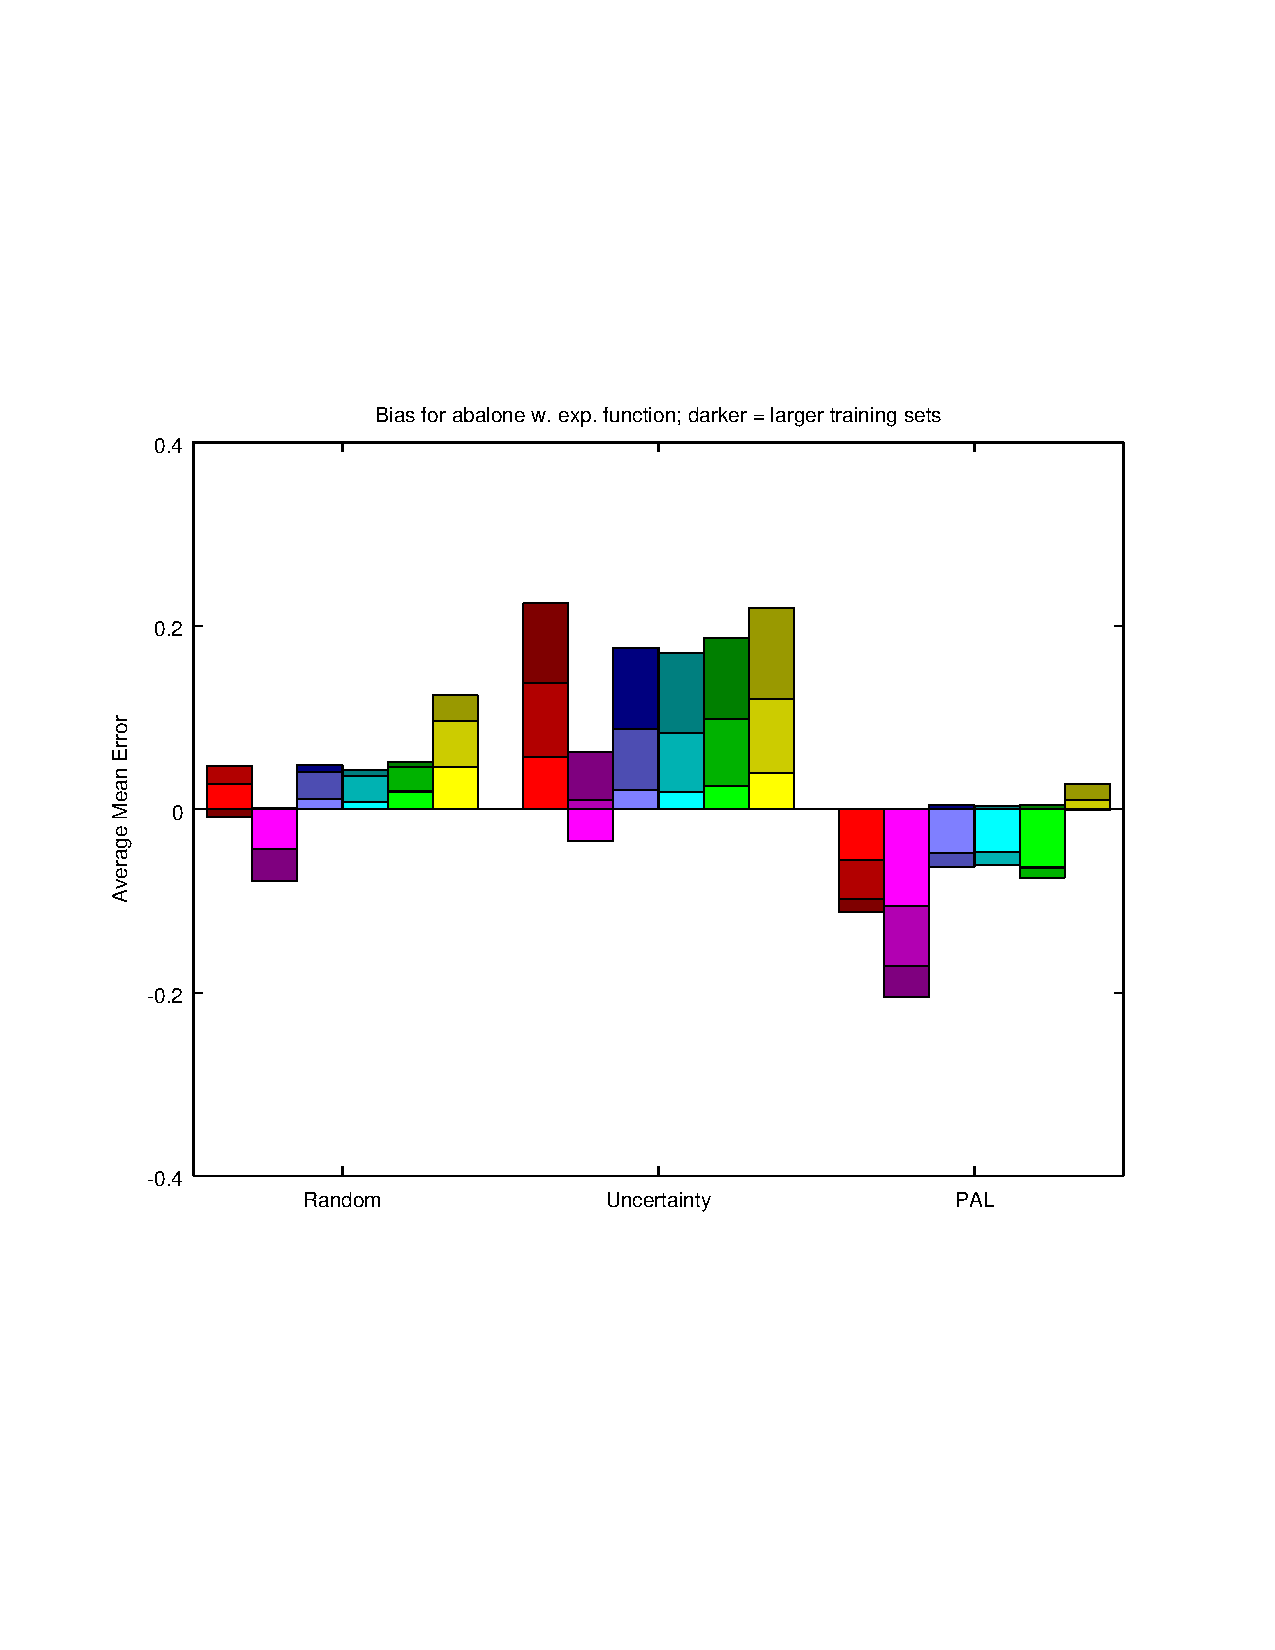
\includegraphics[trim = 1cm 6.5cm 2.5cm 6.5cm, clip = true, width = 0.48\textwidth]{meanErrExpabalone}
	\caption{Average mean errors for the different active learners and datasets using the exponential model. The darker colored bars mark the errors of later learning stages}
	\label{fig:meanErrorsExp}
\end{figure}

Generally, which estimators coupled with a function model show the least bias is both dependent on the dataset as well as the active learner used. That said, some tendencies emerge. For random sampling and training sets of size 16 to 30, \textit{.632+ BS} has the upper hand. Only on the checke1 dataset does it not have the lowest bias; \textit{path} and \textit{pathSuper} with both sigmoid and linear function model as well as \textit{averaged} with the sigmoid model show lower ones. A similar picture can be painted for $k \in [8, 15]$, the difference being it is the abalone set which falls out of line. Here, every other estimator used has a lower or at least equal bias. I attribute this at least partially to an overall increase of estimation performance of the other estimators; the classifier's accuracy hovers around $0.6$ for abalone, only slightly rising for larger training sets. As the study noted, it is possible that the features used are not adequate to predict the age of an abalone. The accuracy estimates thus form some sort of tunnel around $0.6$, giving the function fitting less room, making large mistakes less likely. However, the linear model is only fit with the estimates of the largest four subset sizes; any jitter is picked up by the fitter. As a result, the bias with the linear model, at least for middle-sized training sets, is larger.

The supremacy of \textit{.632+ BS} is broken when regarding the very first few estimates. Here, even the standard \textit{5-Fold CV} shows a lower bias. Whether and which of the other estimators is an improvement differs; the dataset is the most deciding factor. For the 2dData set, both \textit{path} and \textit{pathSuper} with the linear model come close to \textit{.632+ BS}, but do not beat it. They do however beat the \textit{5-Fold CV}. With the sigmoid and exponential model, all shown estimators at least triple the bias of \textit{.632 BS}.

\begin{figure}[h]
	\centering
	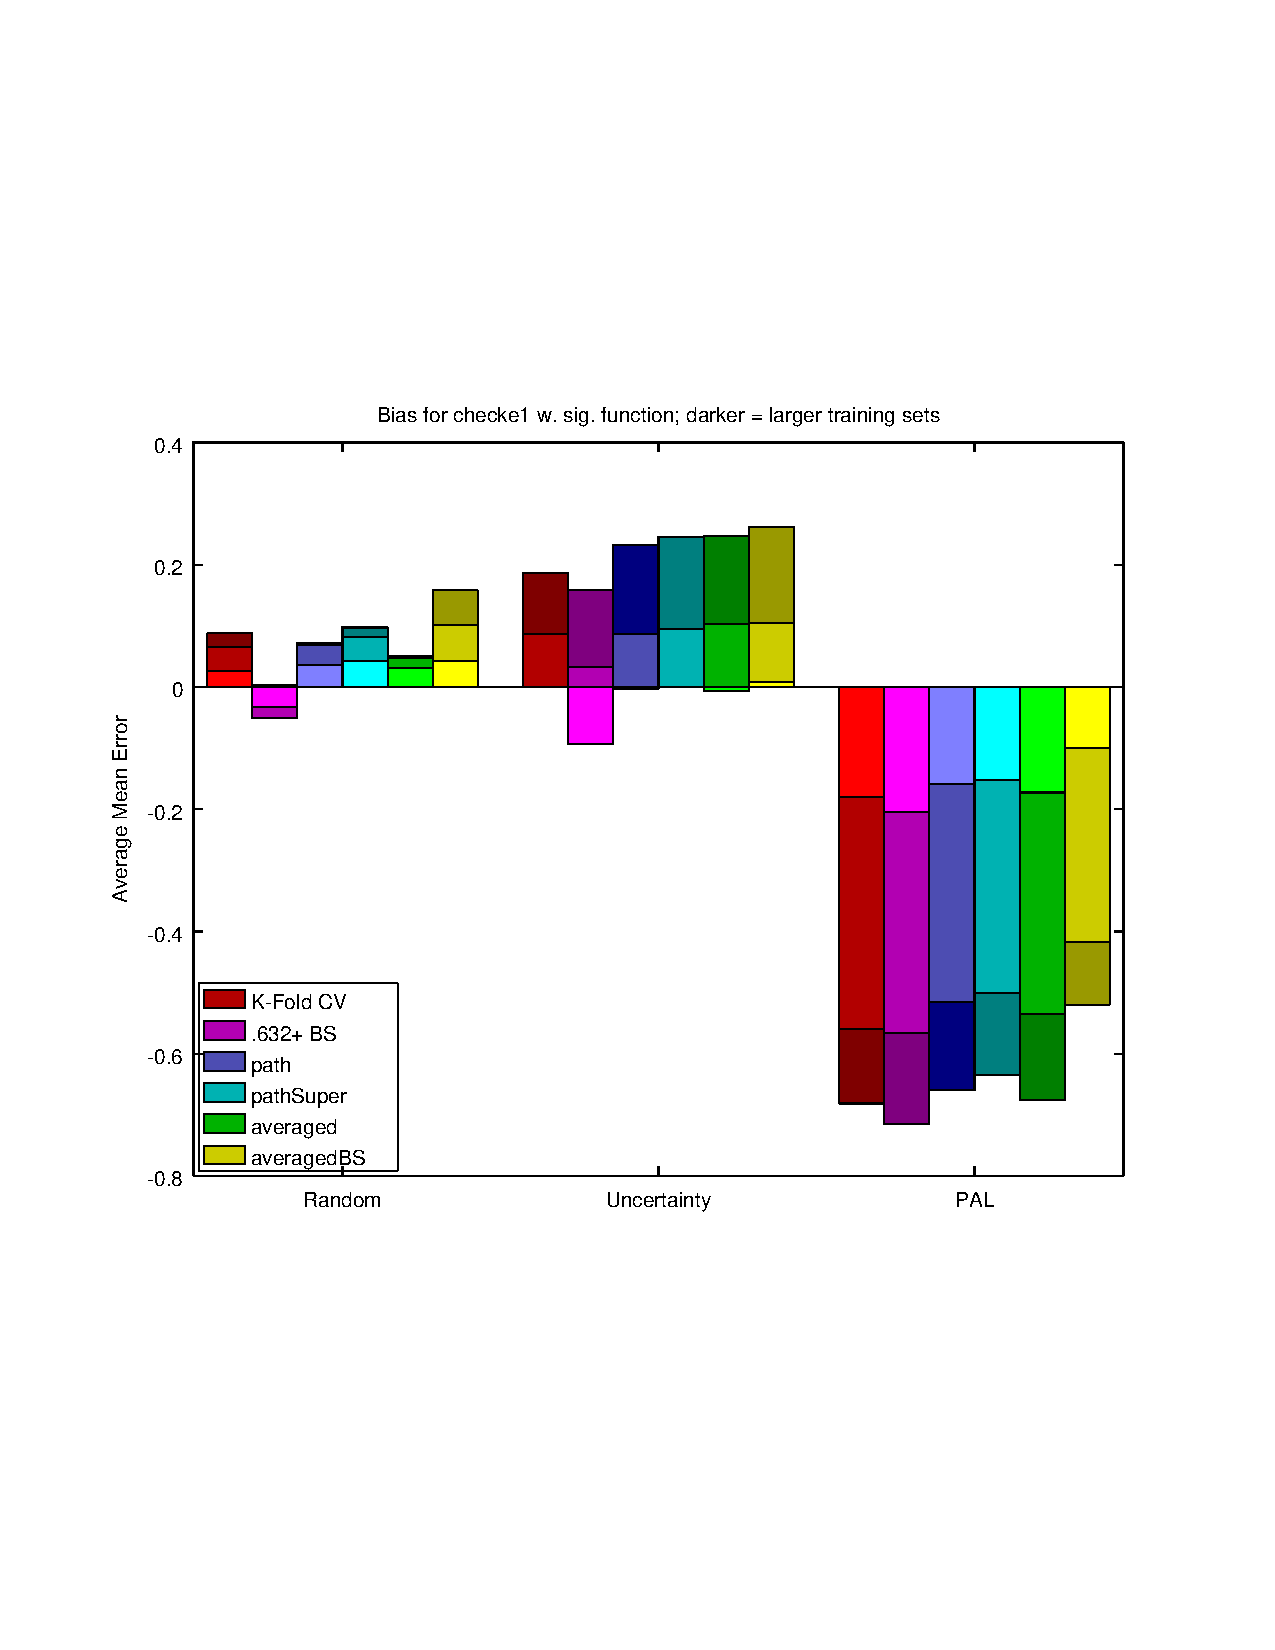
\includegraphics[trim = 1cm 6.5cm 2.5cm 6.5cm, clip = true, width = 0.48\textwidth]{meanErrSigchecke1}
	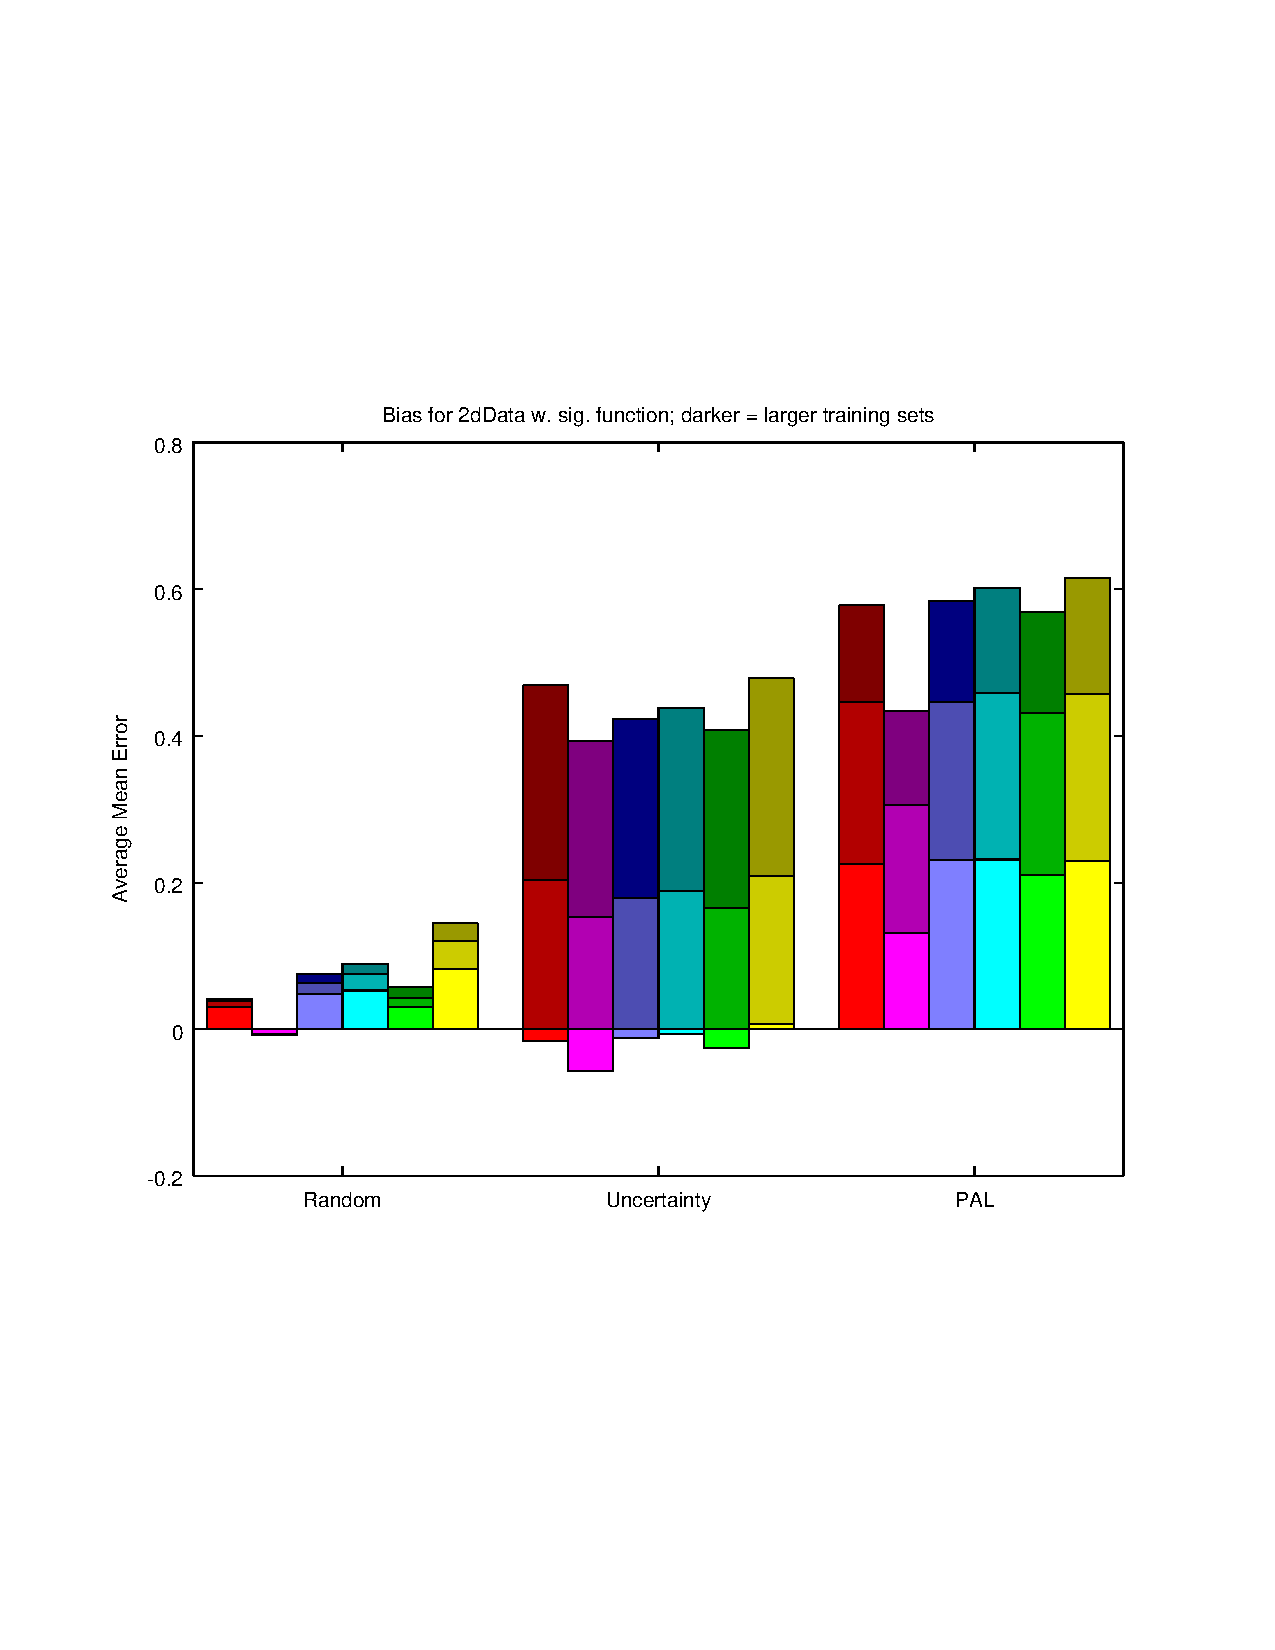
\includegraphics[trim = 1cm 6.5cm 2.5cm 6.5cm, clip = true, width = 0.48\textwidth]{meanErrSig2dData}
	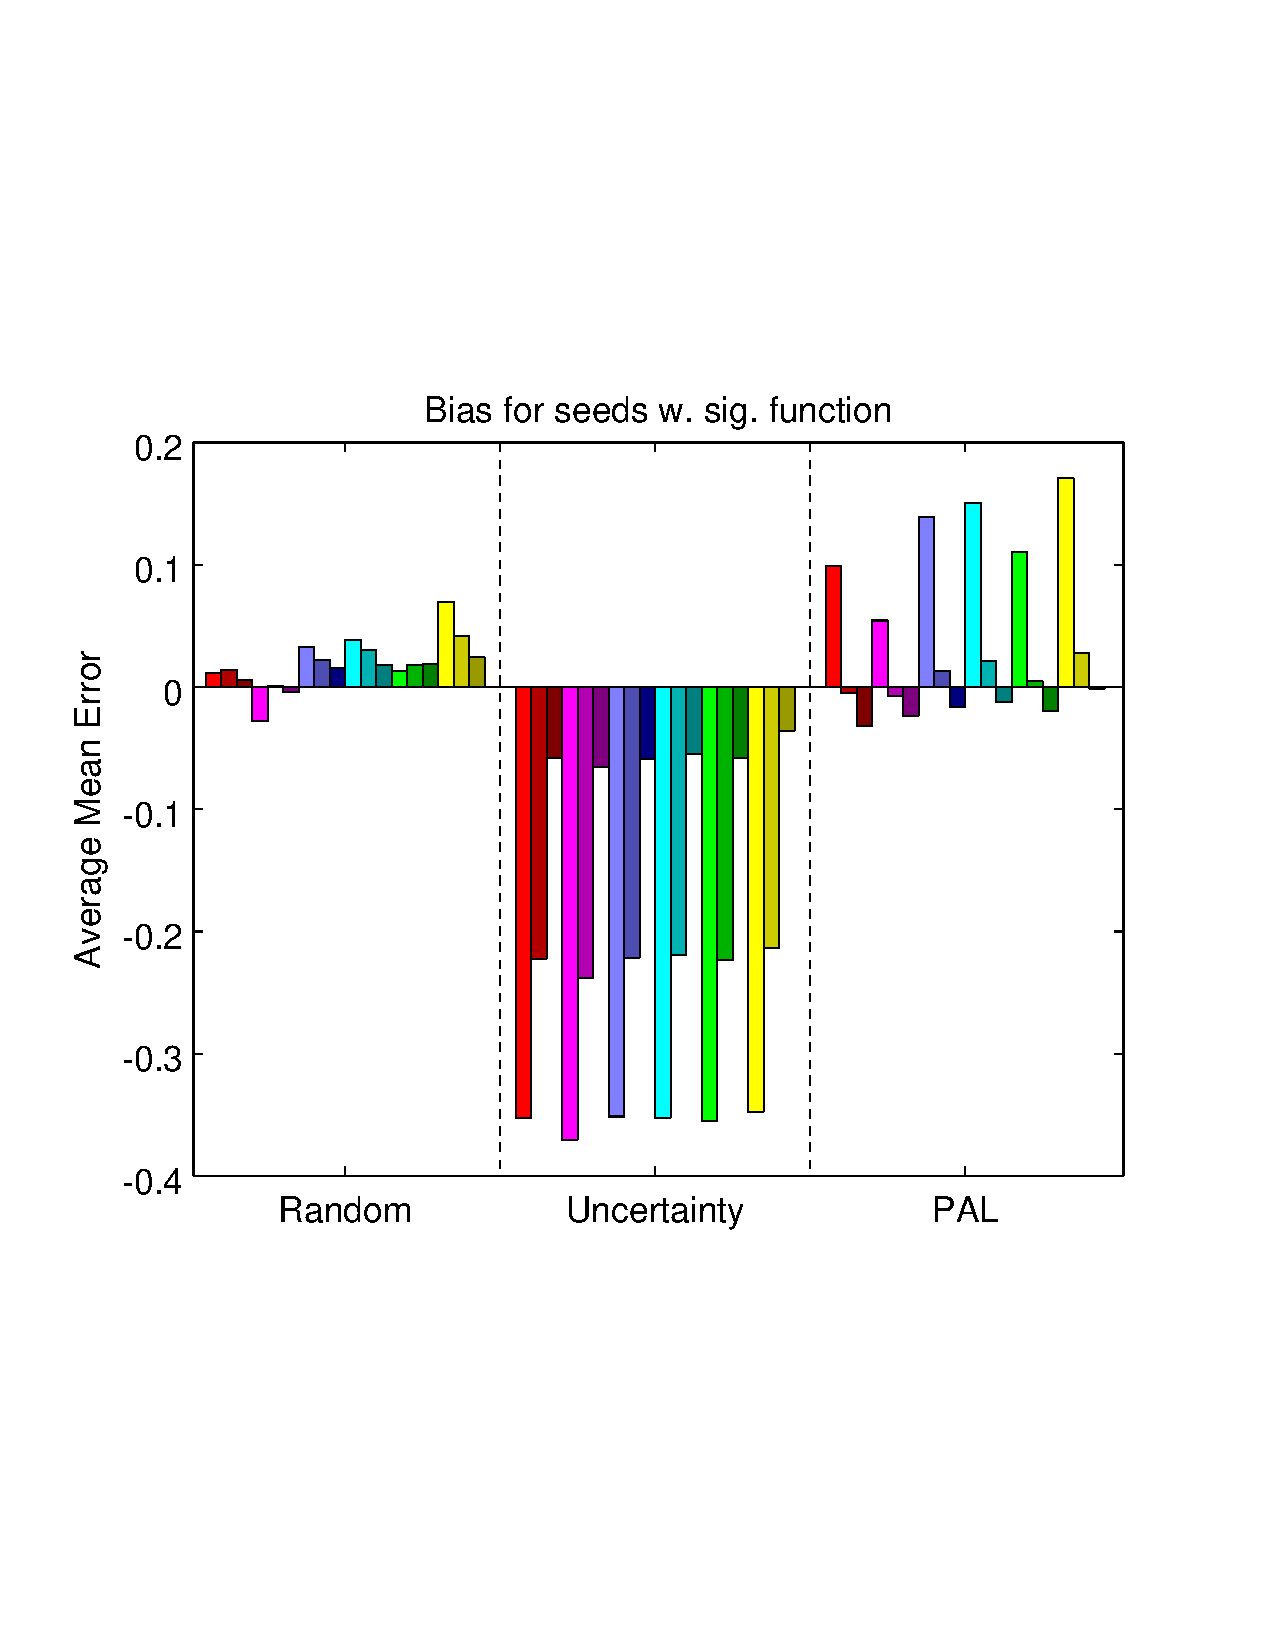
\includegraphics[trim = 1cm 6.5cm 2.5cm 6.5cm, clip = true, width = 0.48\textwidth]{meanErrSigseeds}
	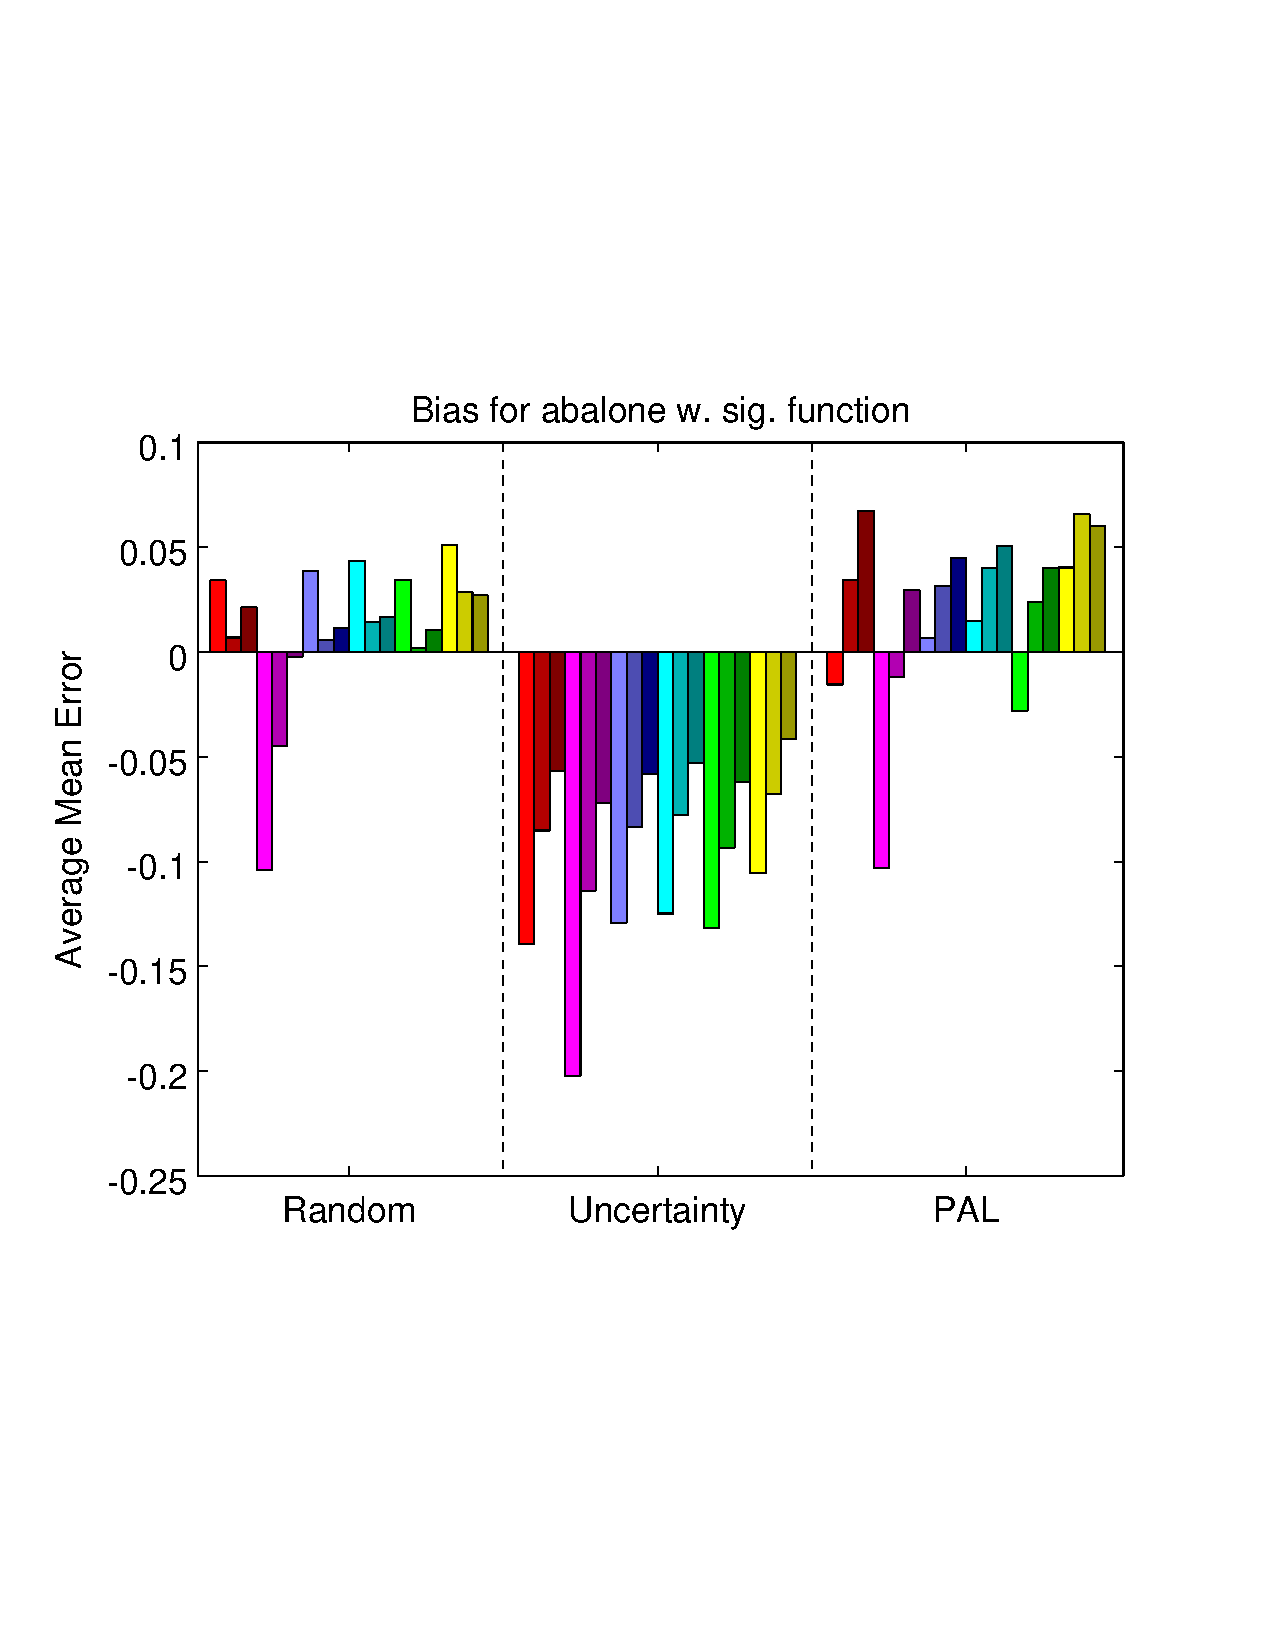
\includegraphics[trim = 1cm 6.5cm 2.5cm 6.5cm, clip = true, width = 0.48\textwidth]{meanErrSigabalone}
	\caption{Average mean errors for the different active learners and datasets using the sigmoid model}
	\label{fig:meanErrorsSig}
\end{figure}

On the flipside, \textit{.632+ BS} is worse than all used estimators for $k \in [3,7]$ with the $checke1$ set, regardless of the function model; the same goes for abalone. What is common to all datasets is the sign of the bias: \textit{.632+ BS} always overestimates the classifier's performance for the first few random label purchases.

For \textit{path} and \textit{pathSuper}, the optimal choice of function is dependent on the training set size. When estimating a classifier with $k \in [3, 7]$, the exponential model is favorable for all sets except 2dData, where the linear model does better. In the later stages, however, the sigmoid model takes over. This is also the case for \textit{averaged}, which overall shows less bias with it. \textit{AveragedBS}, on the other hand, prefers the linear model, with which it offers the lowest overall bias for the first learning stage (with the exception of 2dData).

Shifting the view onto estimation with \textit{uncertainty sampling}, it is obvious that all estimators perform generally worse than they did with random sampling. This discrepancy is caused by the different ways instances are selected: with random sampling, the training instances can be collected from anywhere in the dataset, while uncertainty sampling chooses those that are close to the decision boundary (or what it deems as such). In the case of 2dData, where a fairly clear border exists, this leads to a quick improvement of the classifier's accuracy. However, this poses a difficulty for the estimators, as they keep some of these instances out and test the remaining classifier on them. Since they are close to the border, they also tend to be somewhat noisy, i.e. their class label may be wrong or they are on the wrong sign of the border. This is the case for 2dData, where single outliers (wrongly) drag down the performance estimate. For abalone it is the other way around: using uncertainty sampling results in a relatively poor classifier since there are no two label groups separable by a hyperplane, and the estimation $\widehat{acc}_c$ at the alleged decision boundary is still better than the classifier's true accuracy $acc_c$.

The story is a bit different for the checke1 dataset, where the estimation bias is surprisingly low. Here, uncertainty sampling also imagines a single border that is not real (as it is not the only border). However, the label groups near this border are very uneven in size: looking at \ref{fig:ALillustration}, one checker field is on the inside of a tip-like boundary, and two are close by on the other side. Since the Parzen window classifier also takes into account the total ratio of class labels, instances near the border will be misclassified and thus cross-validation turns up a fairly low estimate, which is close to the similarly low true accuracy $acc_c$. None of the performs consistently better than its peers; that said, \textit{.632+ BS} does especially poorly for $k \in [3,7]$, whereas \textit{averagedBS} with any function model performs best in that category. $k \in [8, 30]$ is very dependent on the dataset and the model, there is no clear victor.

\begin{figure}[h]
	\centering
	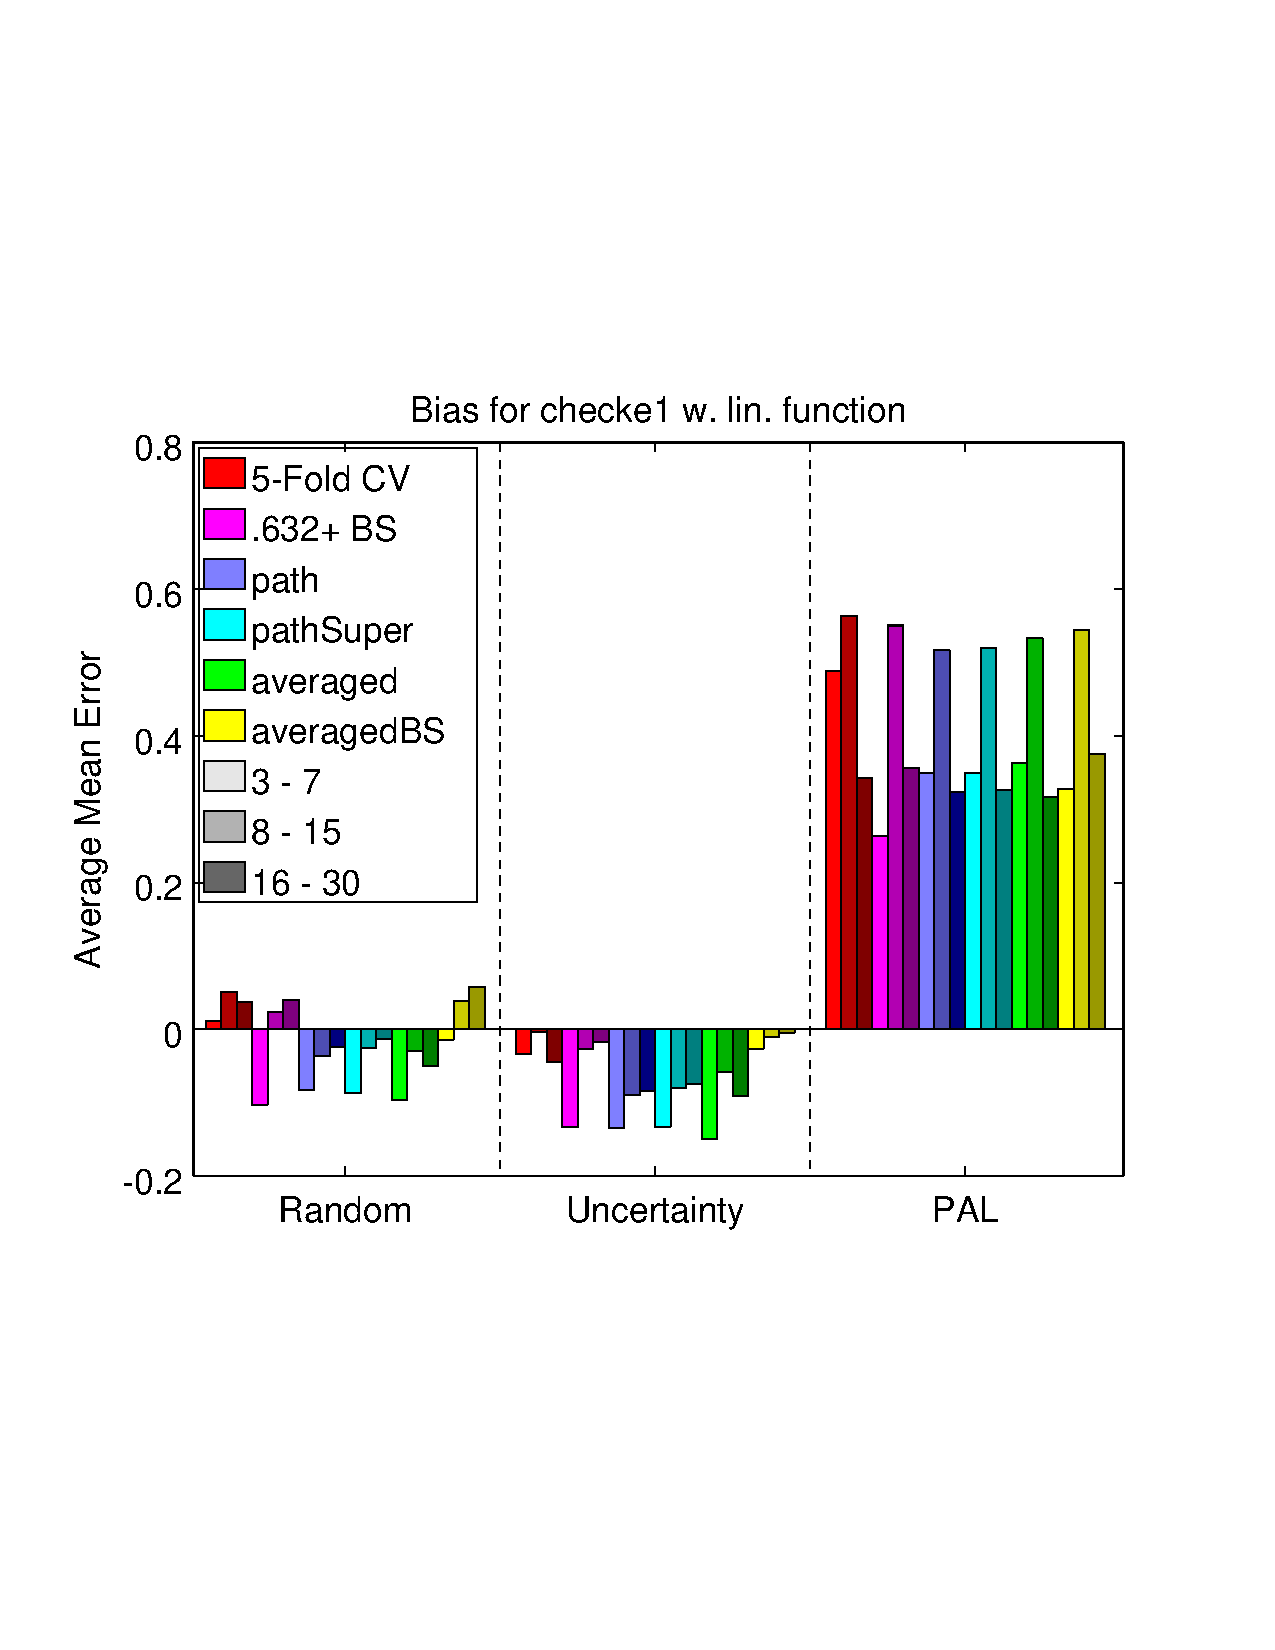
\includegraphics[trim = 1cm 6.5cm 2.5cm 6.5cm, clip = true, width = 0.48\textwidth]{meanErrLinchecke1}
	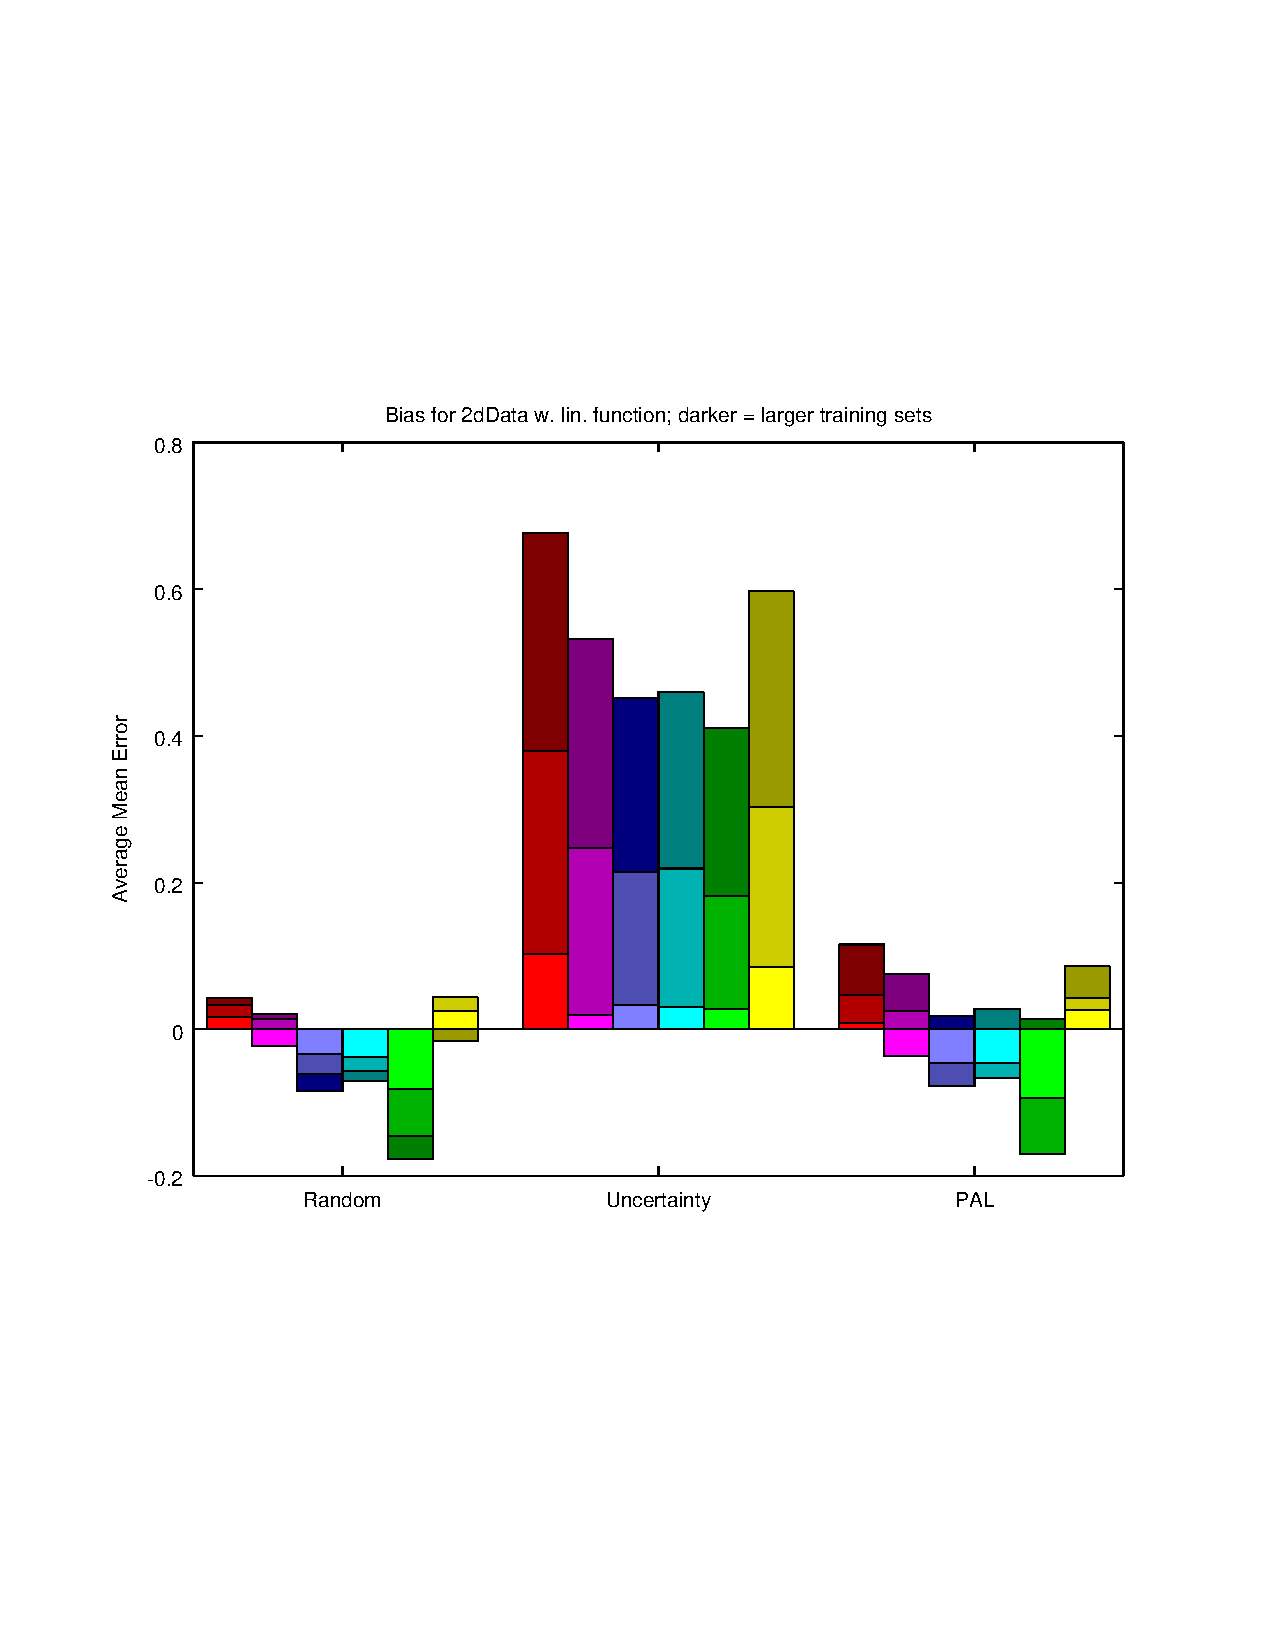
\includegraphics[trim = 1cm 6.5cm 2.5cm 6.5cm, clip = true, width = 0.48\textwidth]{meanErrLin2dData}
	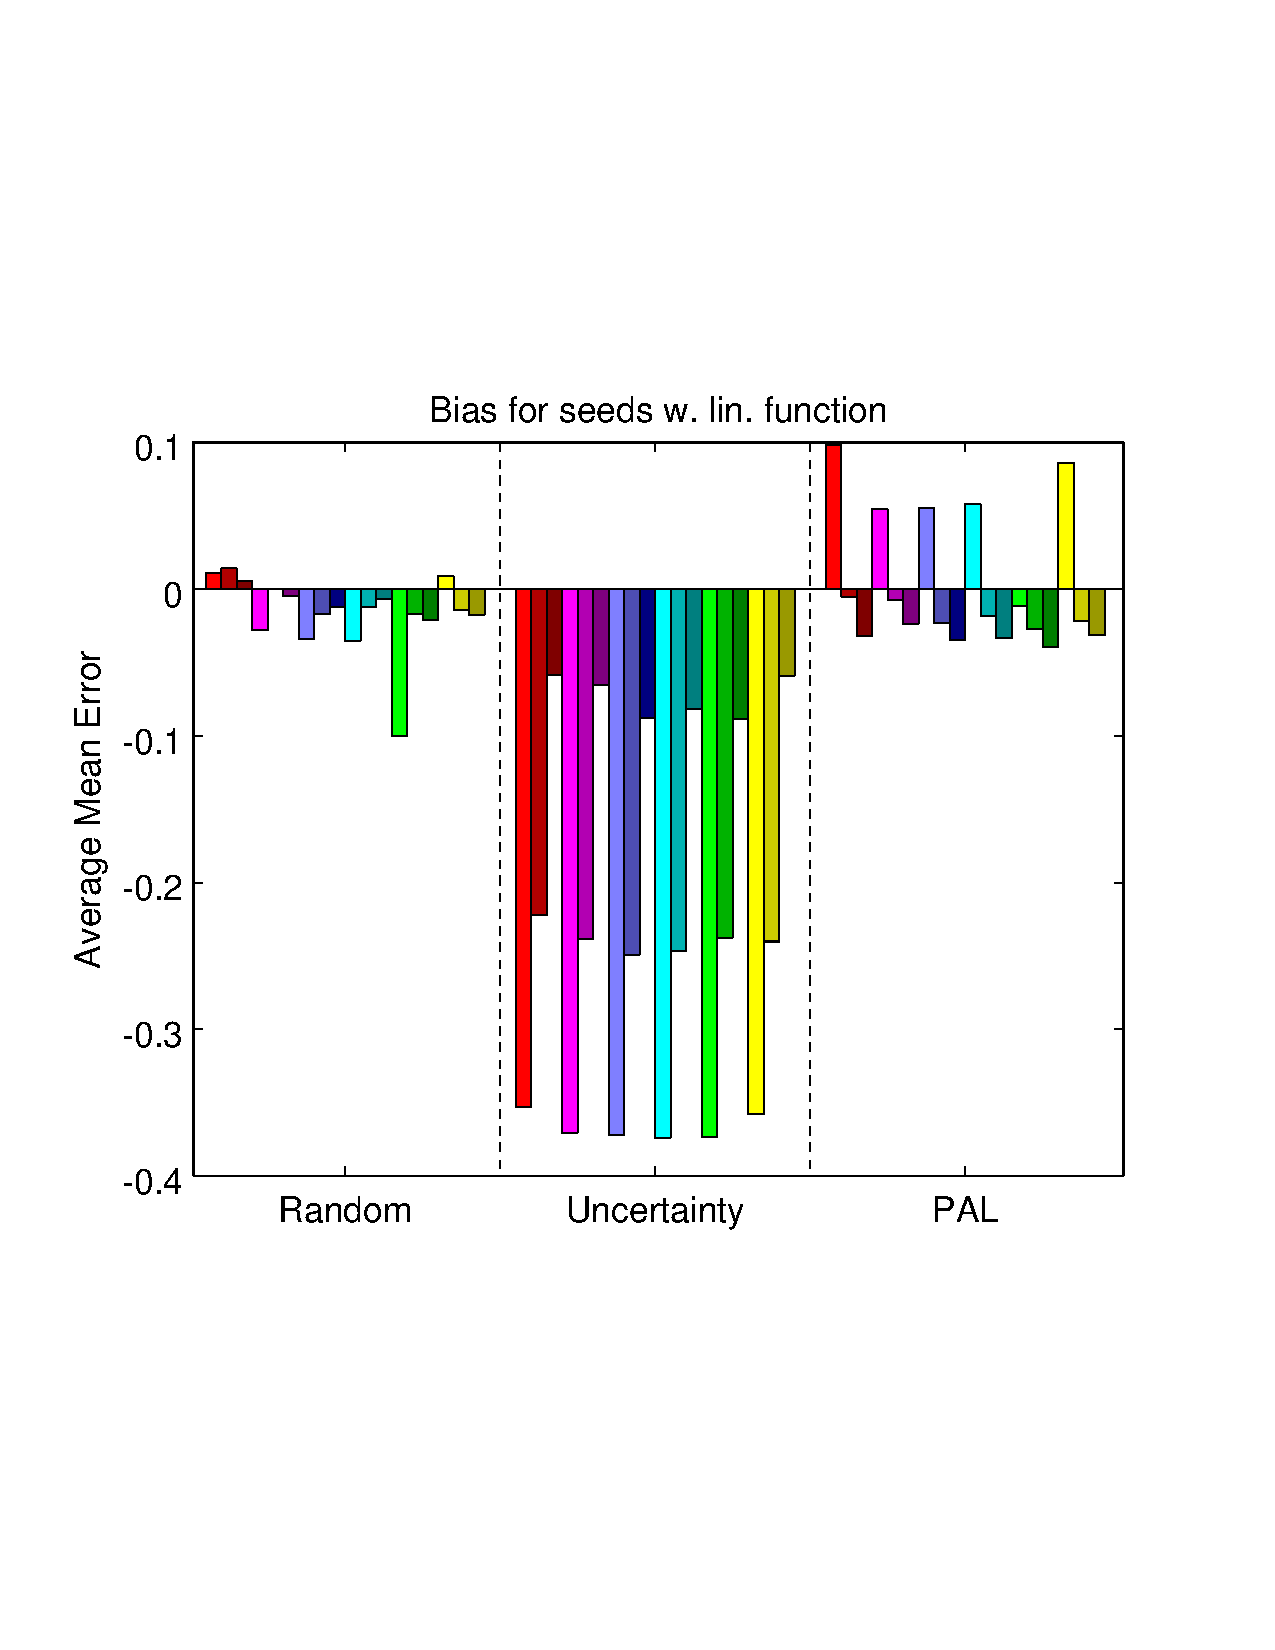
\includegraphics[trim = 1cm 6.5cm 2.5cm 6.5cm, clip = true, width = 0.48\textwidth]{meanErrLinseeds}
	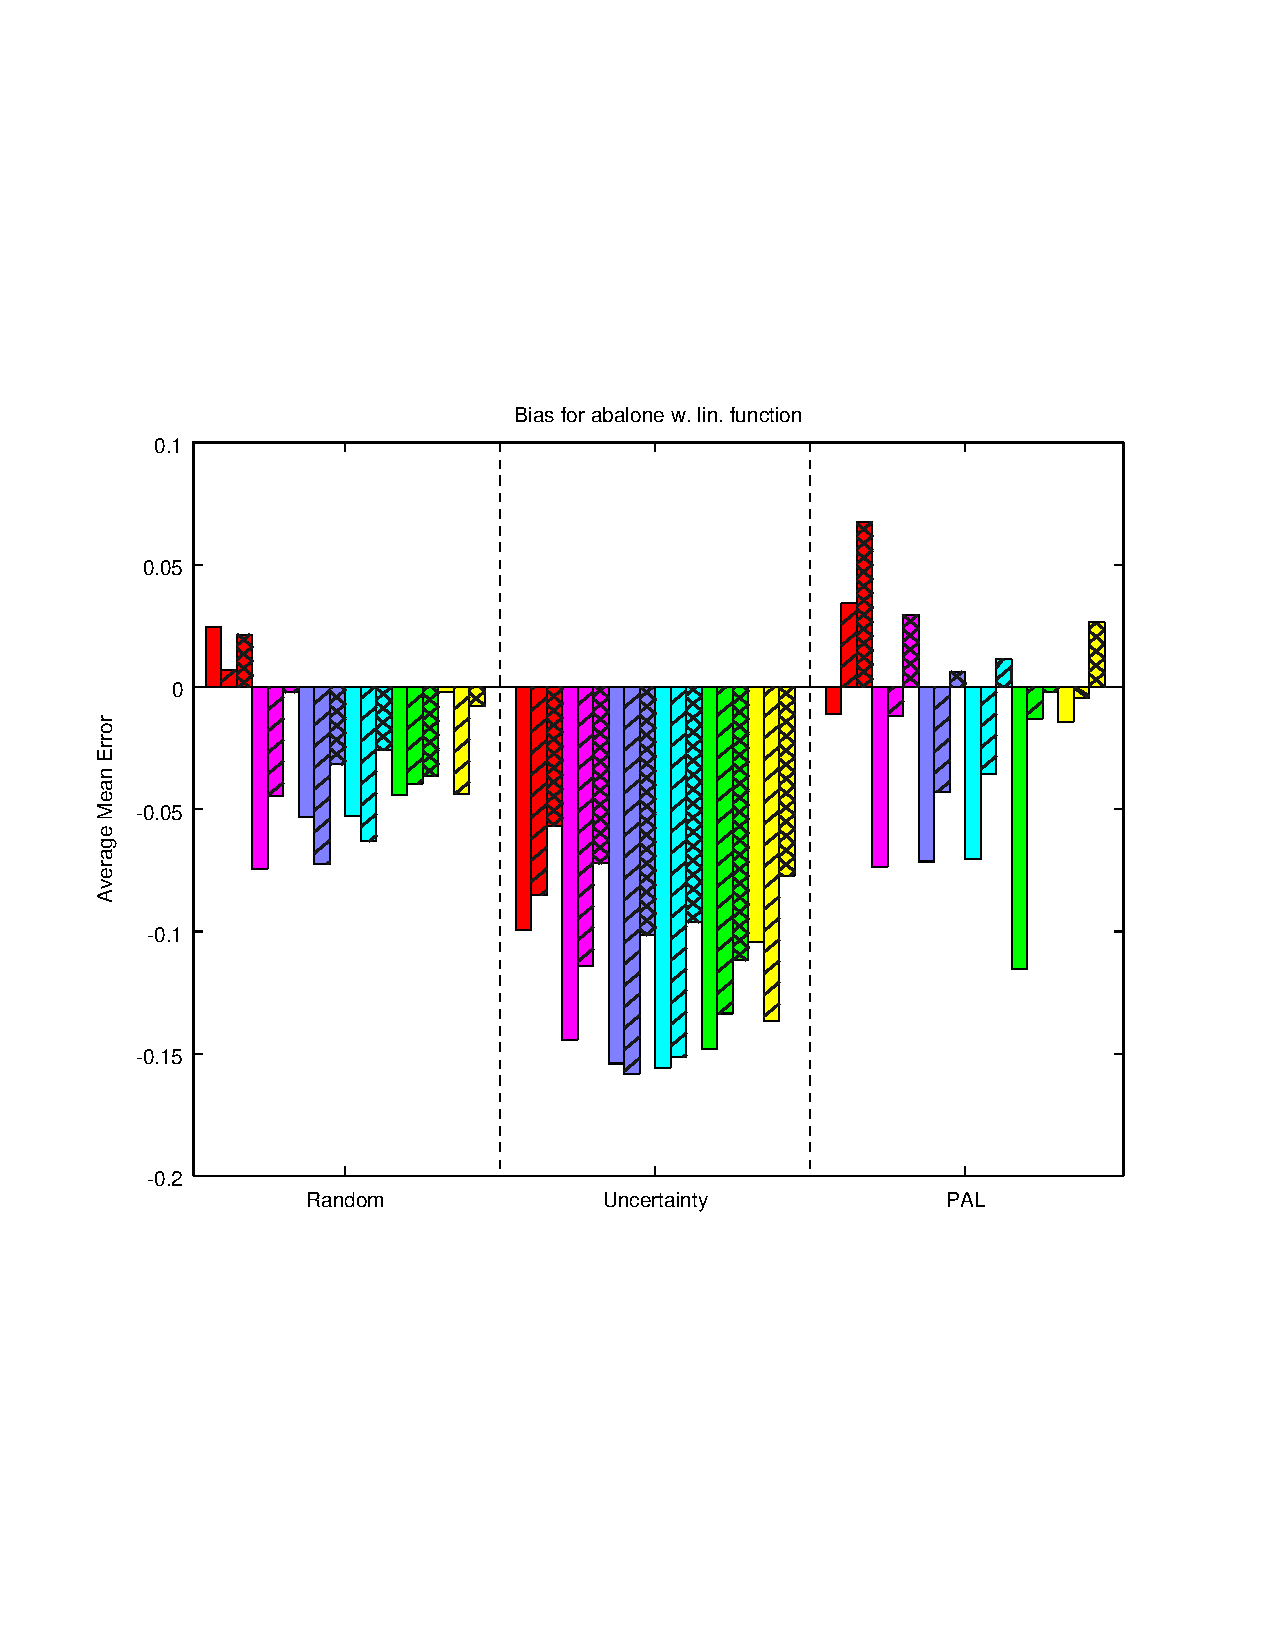
\includegraphics[trim = 1cm 6.5cm 2.5cm 6.5cm, clip = true, width = 0.48\textwidth]{meanErrLinabalone}
	\caption{Average mean errors for the different active learners and datasets using the linear model}
	\label{fig:meanErrorsLin}
\end{figure}

With PAL, the estimators face a similar problem as with uncertainty sampling. With its preference to spread the purchases out to areas with low label, but high instance density, as well as those with unsettled disputes about the predominant class label, it causes steep discrepancies in knowledge between a classifier trained on all $k$ instances and one that only gets $k-1$. Taking a look at the checke1 dataset and \ref{fig:ALillustration} again, it becomes clear that taking away only one instance, the knowledge of a whole checker field may vanish. Of course, a Parzen window classifier would then classify the left-out instance wrong. Since this is the case for most of the instances, the resulting estimation is absurdly low. This effect is not as bad for the seeds and abalone sets as both have fairly flat learning curves. For seeds, very few instances are enough to almost perfectly classify any instance of the dataset, which is due to its very clean label groups. After that, adding new instances provides little additional information, but the first few labels are still important, which is why the bias of all estimators is much higher for $k \in [3,7]$. In the case of abalone, the dependence between features and class label is rather weak, thus an increase in training set size is not that effective.

Which estimator offers the lowest bias is not clear; \textit{.632+ BS} performs the most consistent, but is occasionally overshadowed. Also, using linear fit at least decreases the bias in the early learning stage to levels below that of \textit{5-Fold CV}. The exception is, again, abalone, where it actually offers the lowest bias.

\begin{figure}[h]
	\centering
	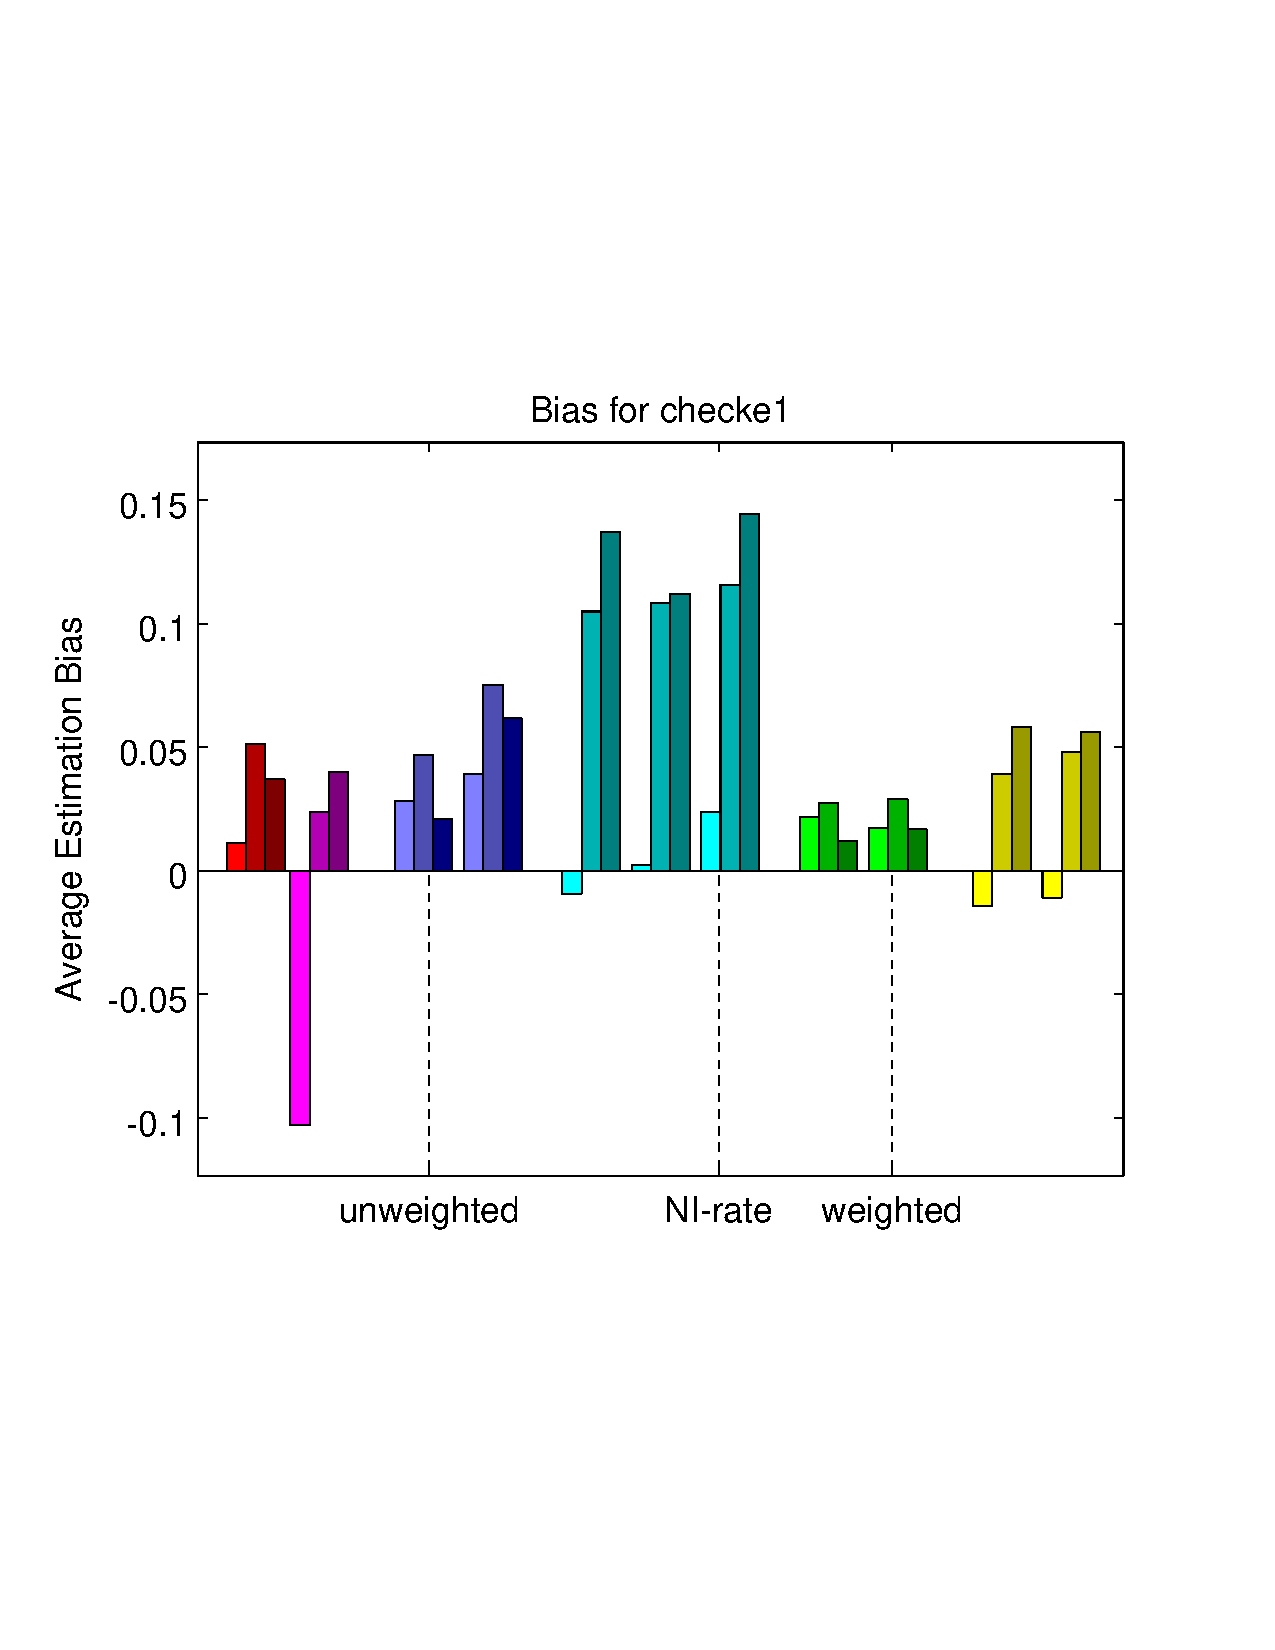
\includegraphics[trim = 0.8cm 6.5cm 2.5cm 6.5cm, clip = true, width = 0.48\textwidth]{meanErrWeightingchecke1}
	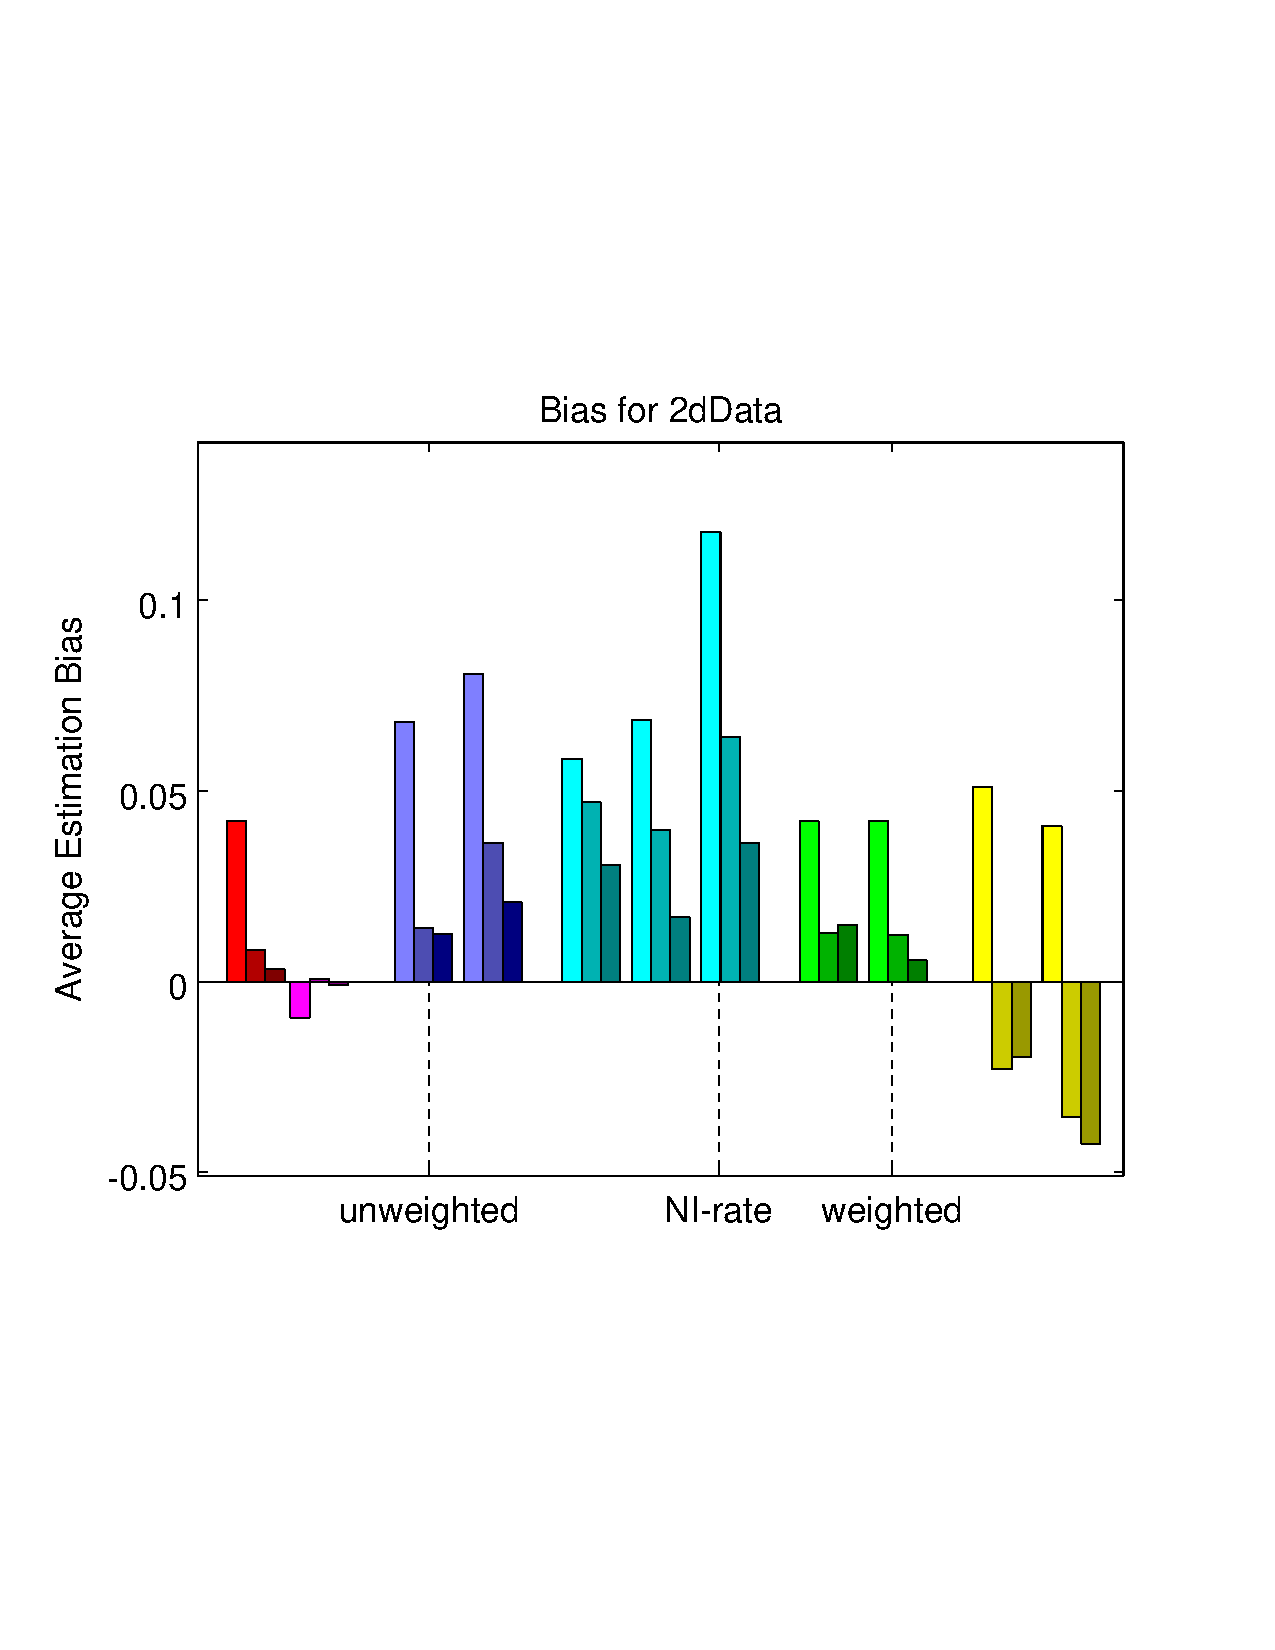
\includegraphics[trim = 0.8cm 6.5cm 2.5cm 6.5cm, clip = true, width = 0.48\textwidth]{meanErrWeighting2dData}
	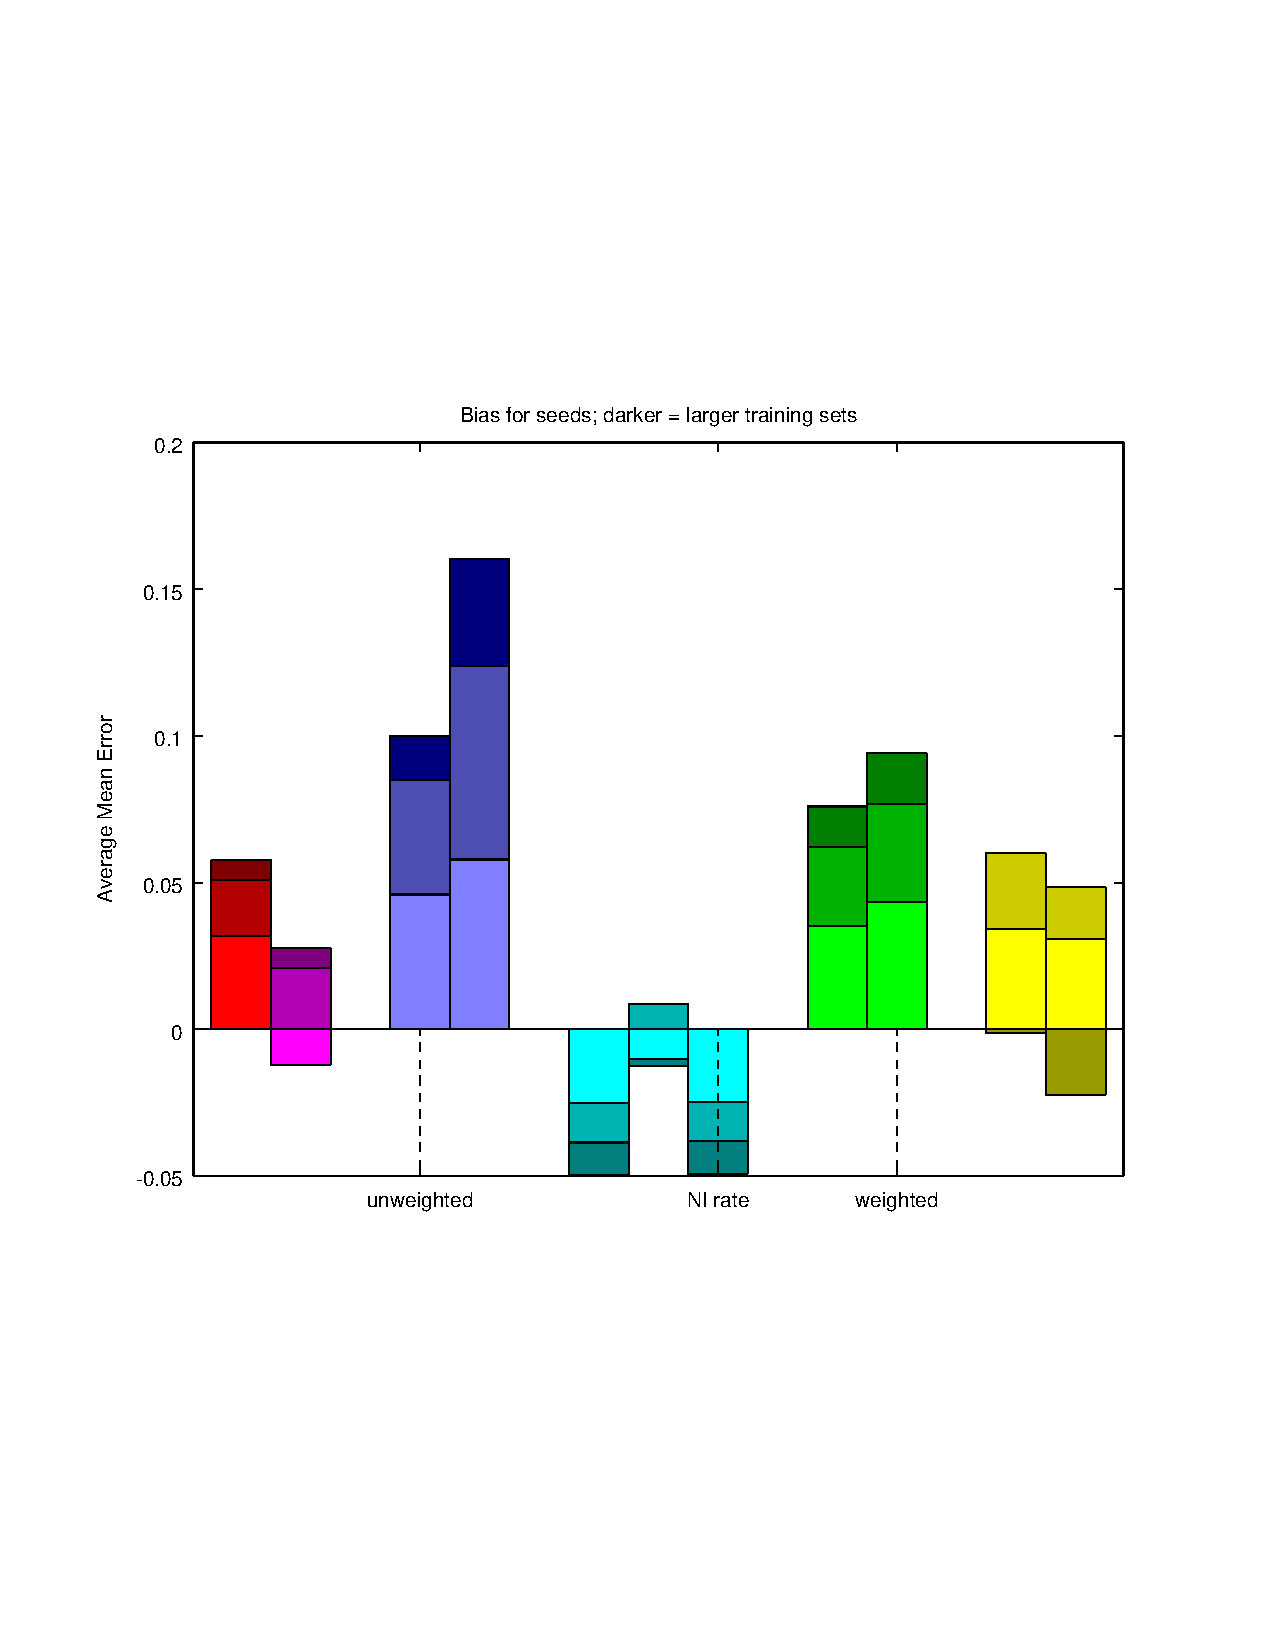
\includegraphics[trim = 0.8cm 6.5cm 2.5cm 6.5cm, clip = true, width = 0.48\textwidth]{meanErrWeightingseeds}
	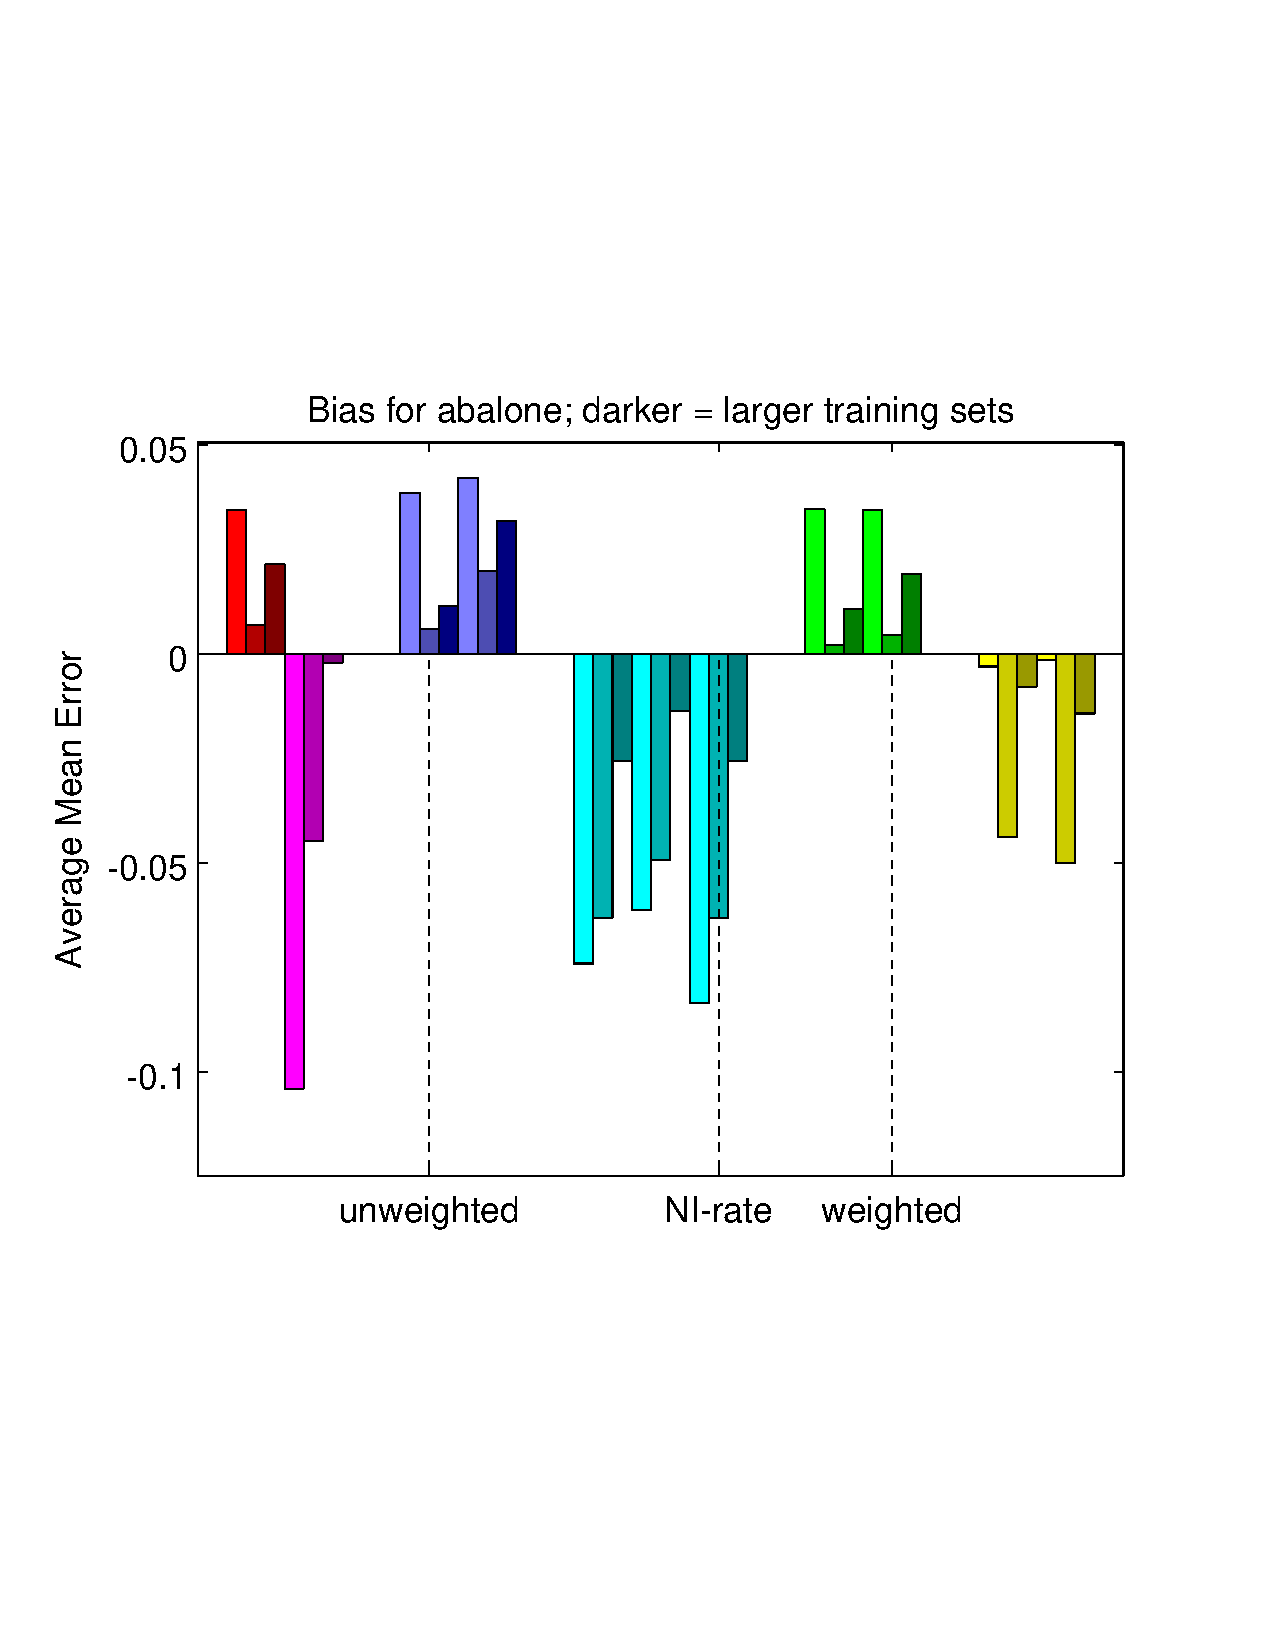
\includegraphics[trim = 0.8cm 6.5cm 2.5cm 6.5cm, clip = true, width = 0.48\textwidth]{meanErrWeightingabalone}
	\caption{Average mean errors for different datasets with random sampling}
	\label{fig:meanErrorsWeighted}
\end{figure}

\paragraph{Statistical weighting}
To identify what role the addition of weights or no-information rate to the fitting have, \ref{fig:meanErrorsWeighted} shows a direct comparison of four of the estimators: \textit{pathSuper} with exponential, \textit{path} and \textit{averaged} with sigmoid and \textit{averagedBS} with the linear function model.

The obvious first: adding an estimate for set size zero corresponding to the estimated no-information rate does not benefit the \textit{pathSuper} method with exponential model at all. On the contrary, it worsens the bias across all datasets and learning stages. This effect is not as distinctive for the other function models, but \textit{pathSuper} synergizes more with $f_{exp.}$, yielding a lower bias especially for the early learning stage. Thus, the results are not depicted here.

Statistical weighting produces more mixed results. \textit{path} does not benefit at all, while \textit{pathSuper} and \textit{averaged} show reduced bias for the later learning stage with $k \in [16,30]$. The former also mostly improves for $k \in [8,15]$, while \textit{averaged} slightly worsens there. The exact opposite is the case for \textit{averagedBS}: its bias reduces for the early stage but worsens later on. A possible explanation is the different function model; \textit{averagedBS} definitely performs better with the linear model.

\subsection{Average squared error}

The error spread is quite a bit lower on the priority list than the estimation bias. To keep the evaluation within a reasonable frame, \ref{fig:squaredErrors} only shows the average squared error for the estimators and associated function models already used in \ref{fig:meanErrorsWeighted}. Each bar holds the error of one estimator, while its subsections indicate the share each learning stage brings to the total mean.

\begin{figure}[h]
	\centering
	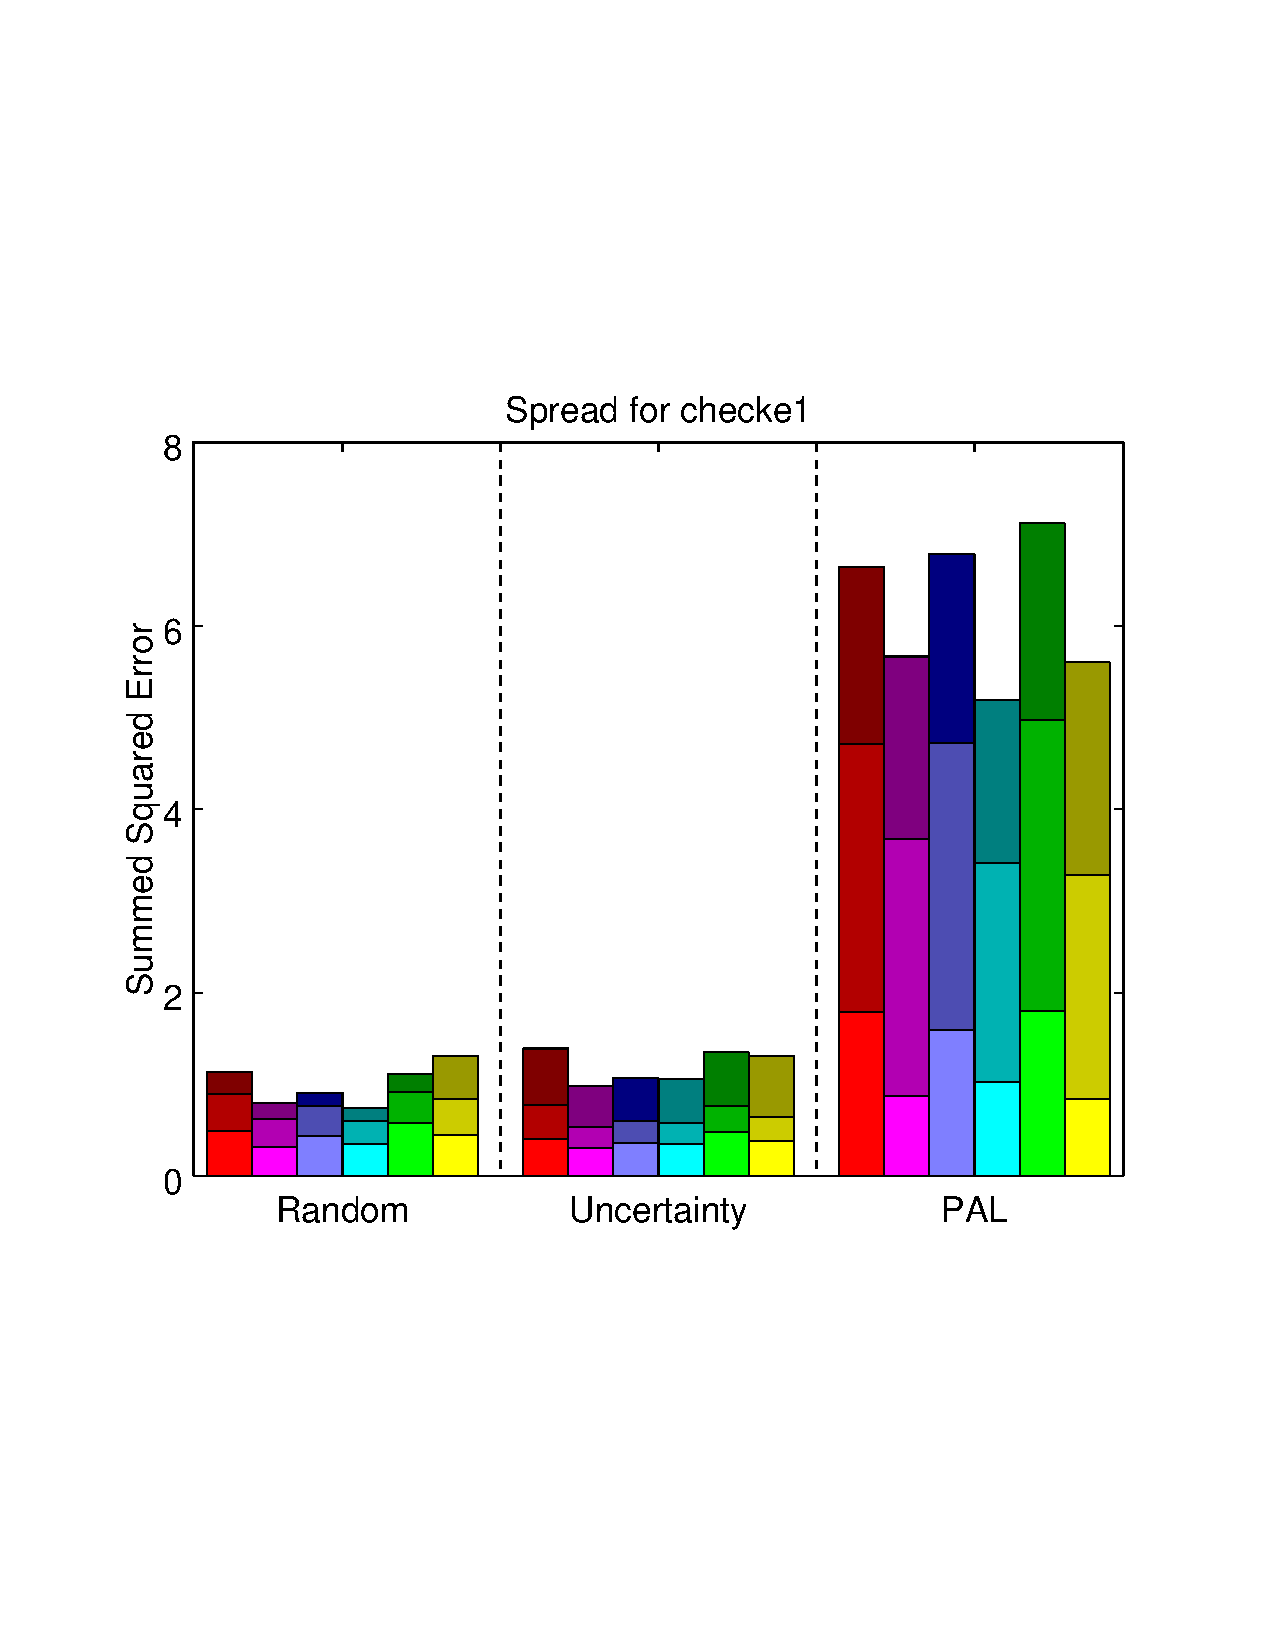
\includegraphics[trim = 0.8cm 6.5cm 2.5cm 6.5cm, clip = true, width = 0.48\textwidth]{squErrchecke1}
	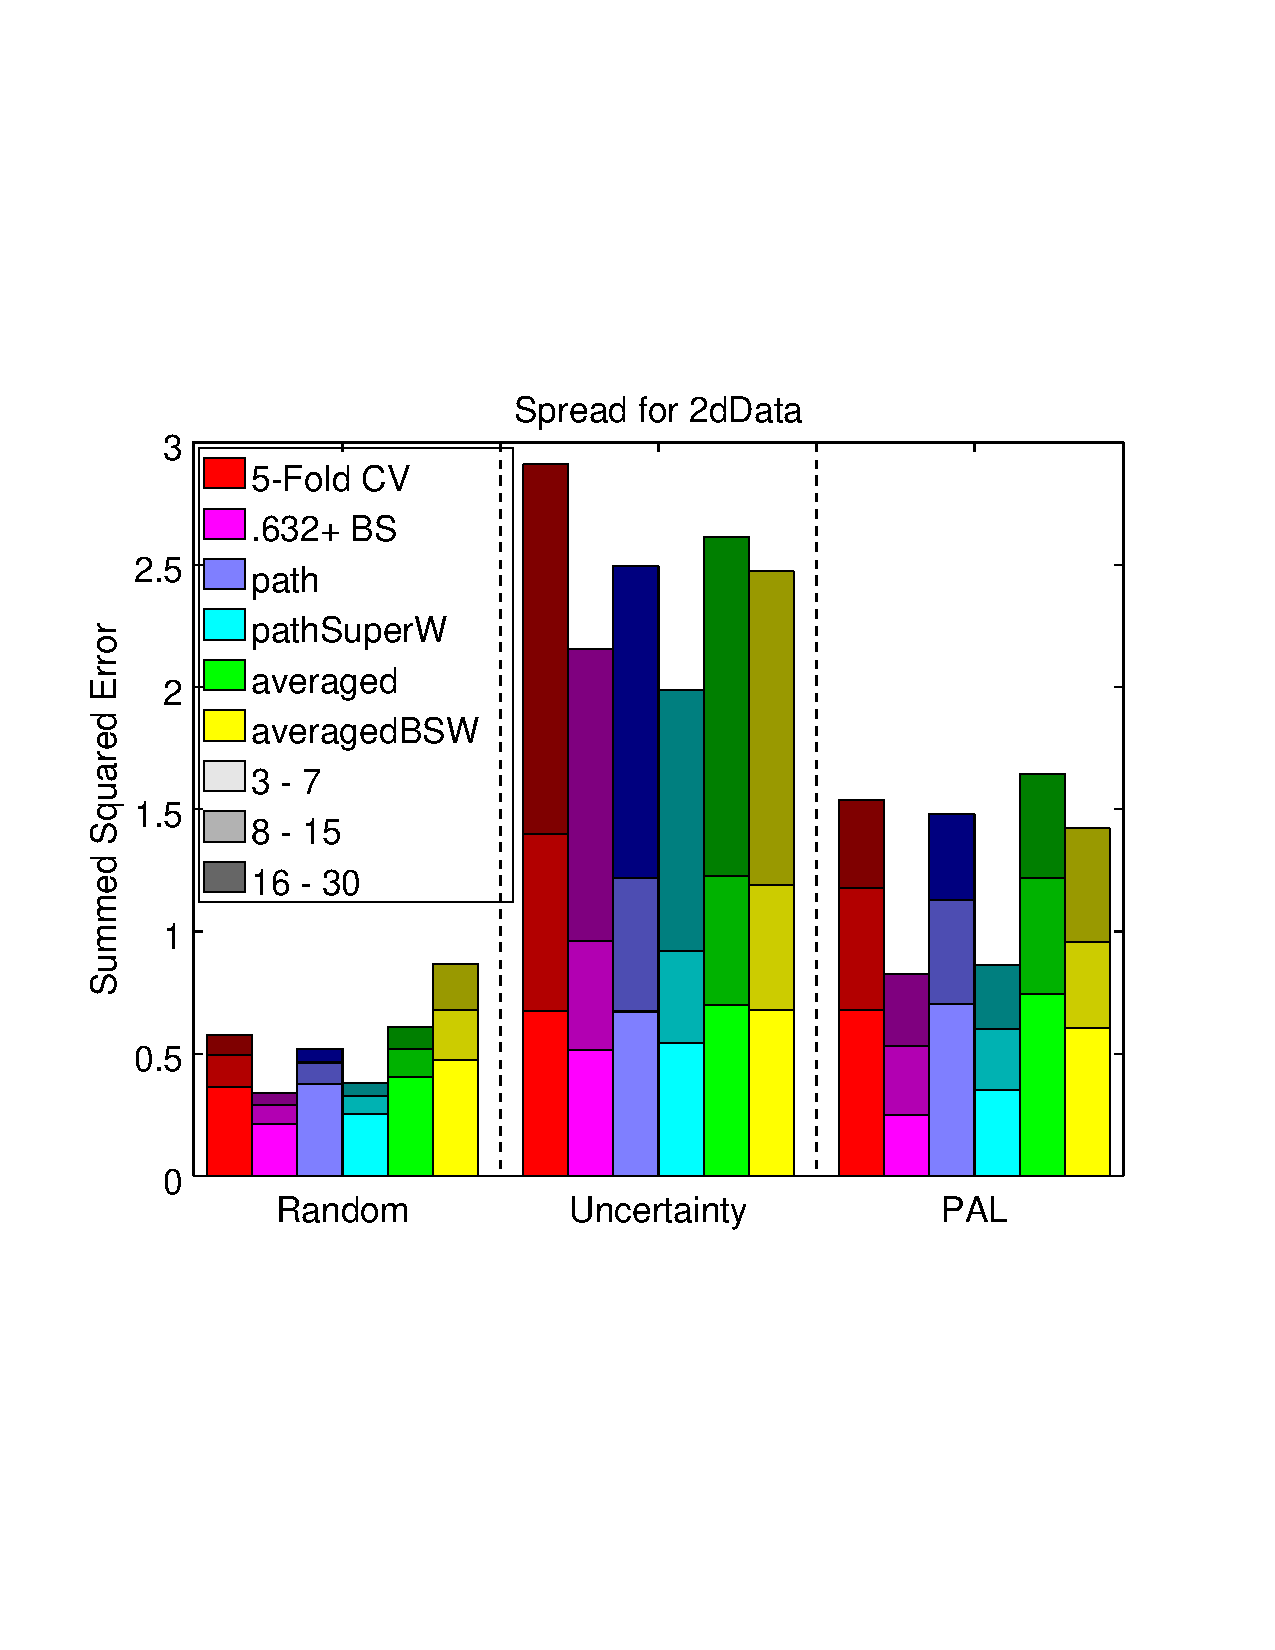
\includegraphics[trim = 0.8cm 6.5cm 2.5cm 6.5cm, clip = true, width = 0.48\textwidth]{squErr2dData}
	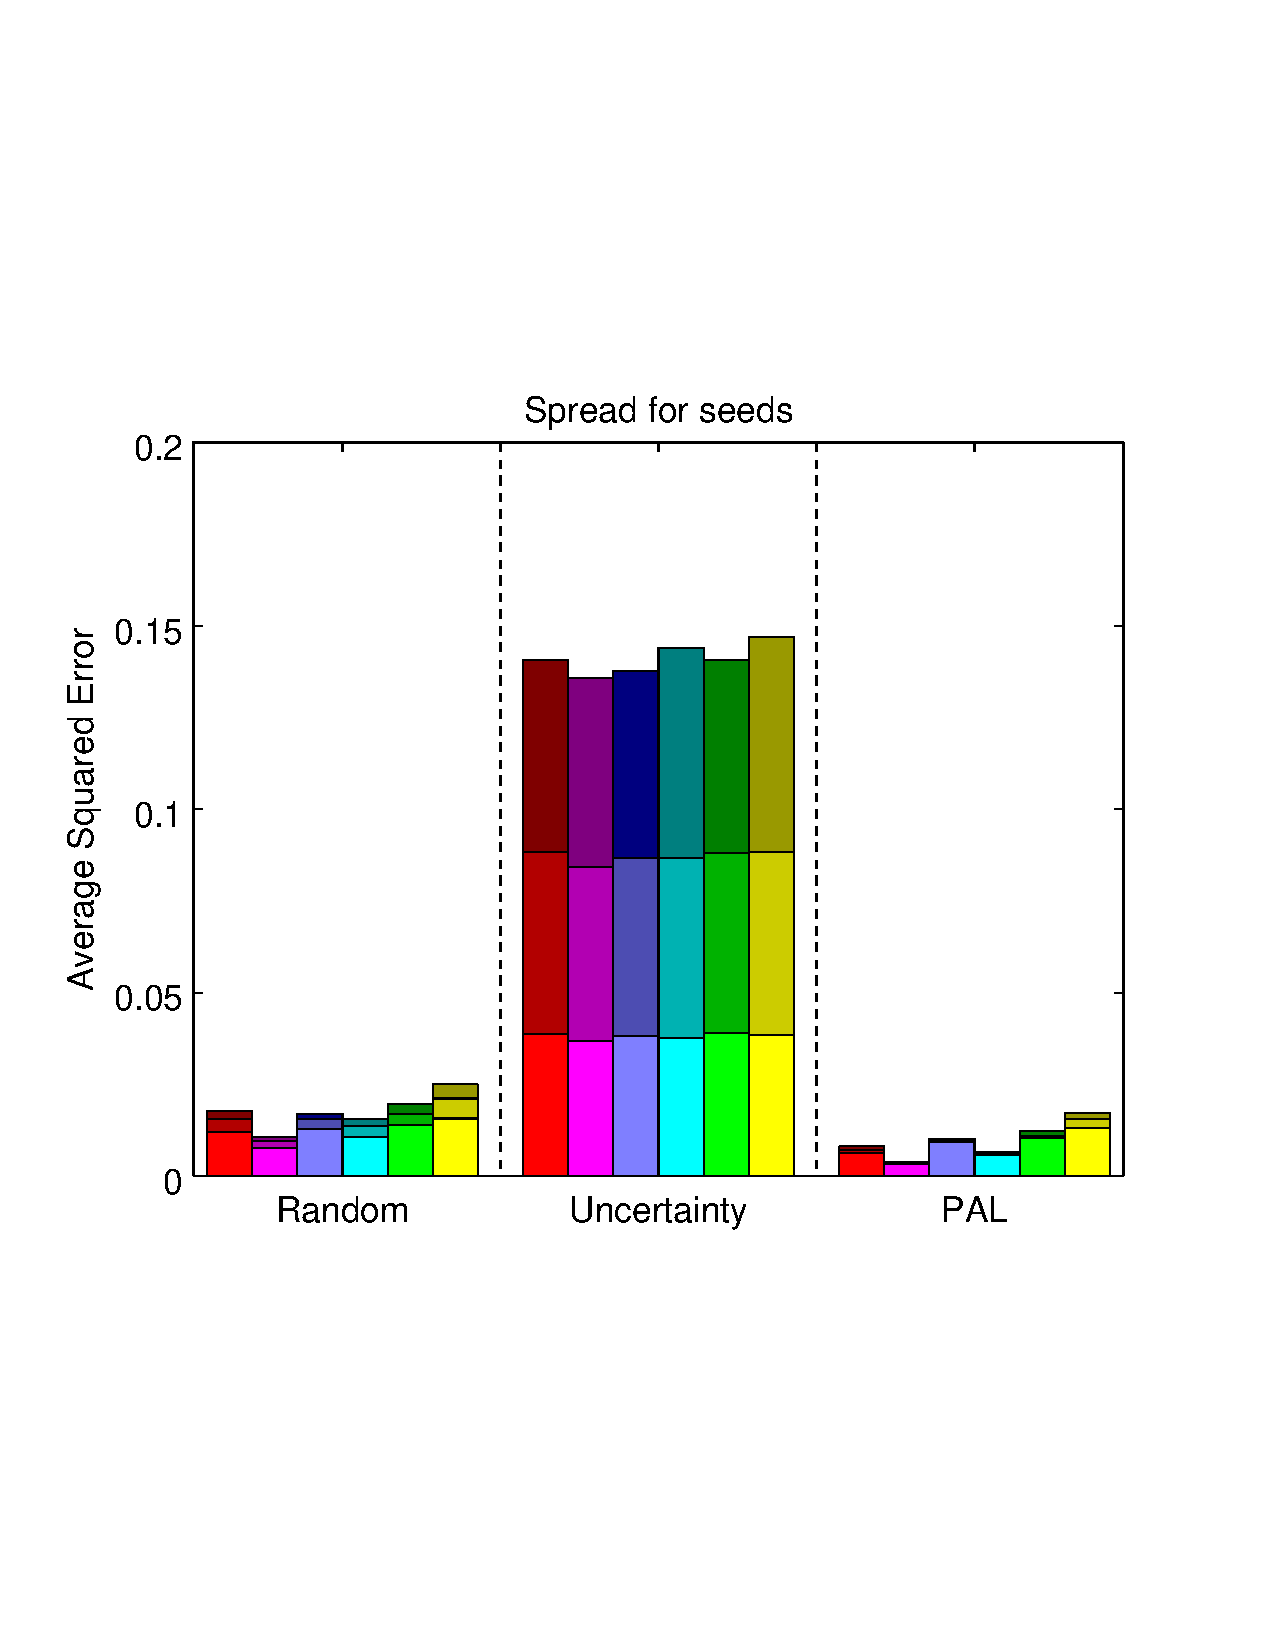
\includegraphics[trim = 0.8cm 6.5cm 2.5cm 6.5cm, clip = true, width = 0.48\textwidth]{squErrseeds}
	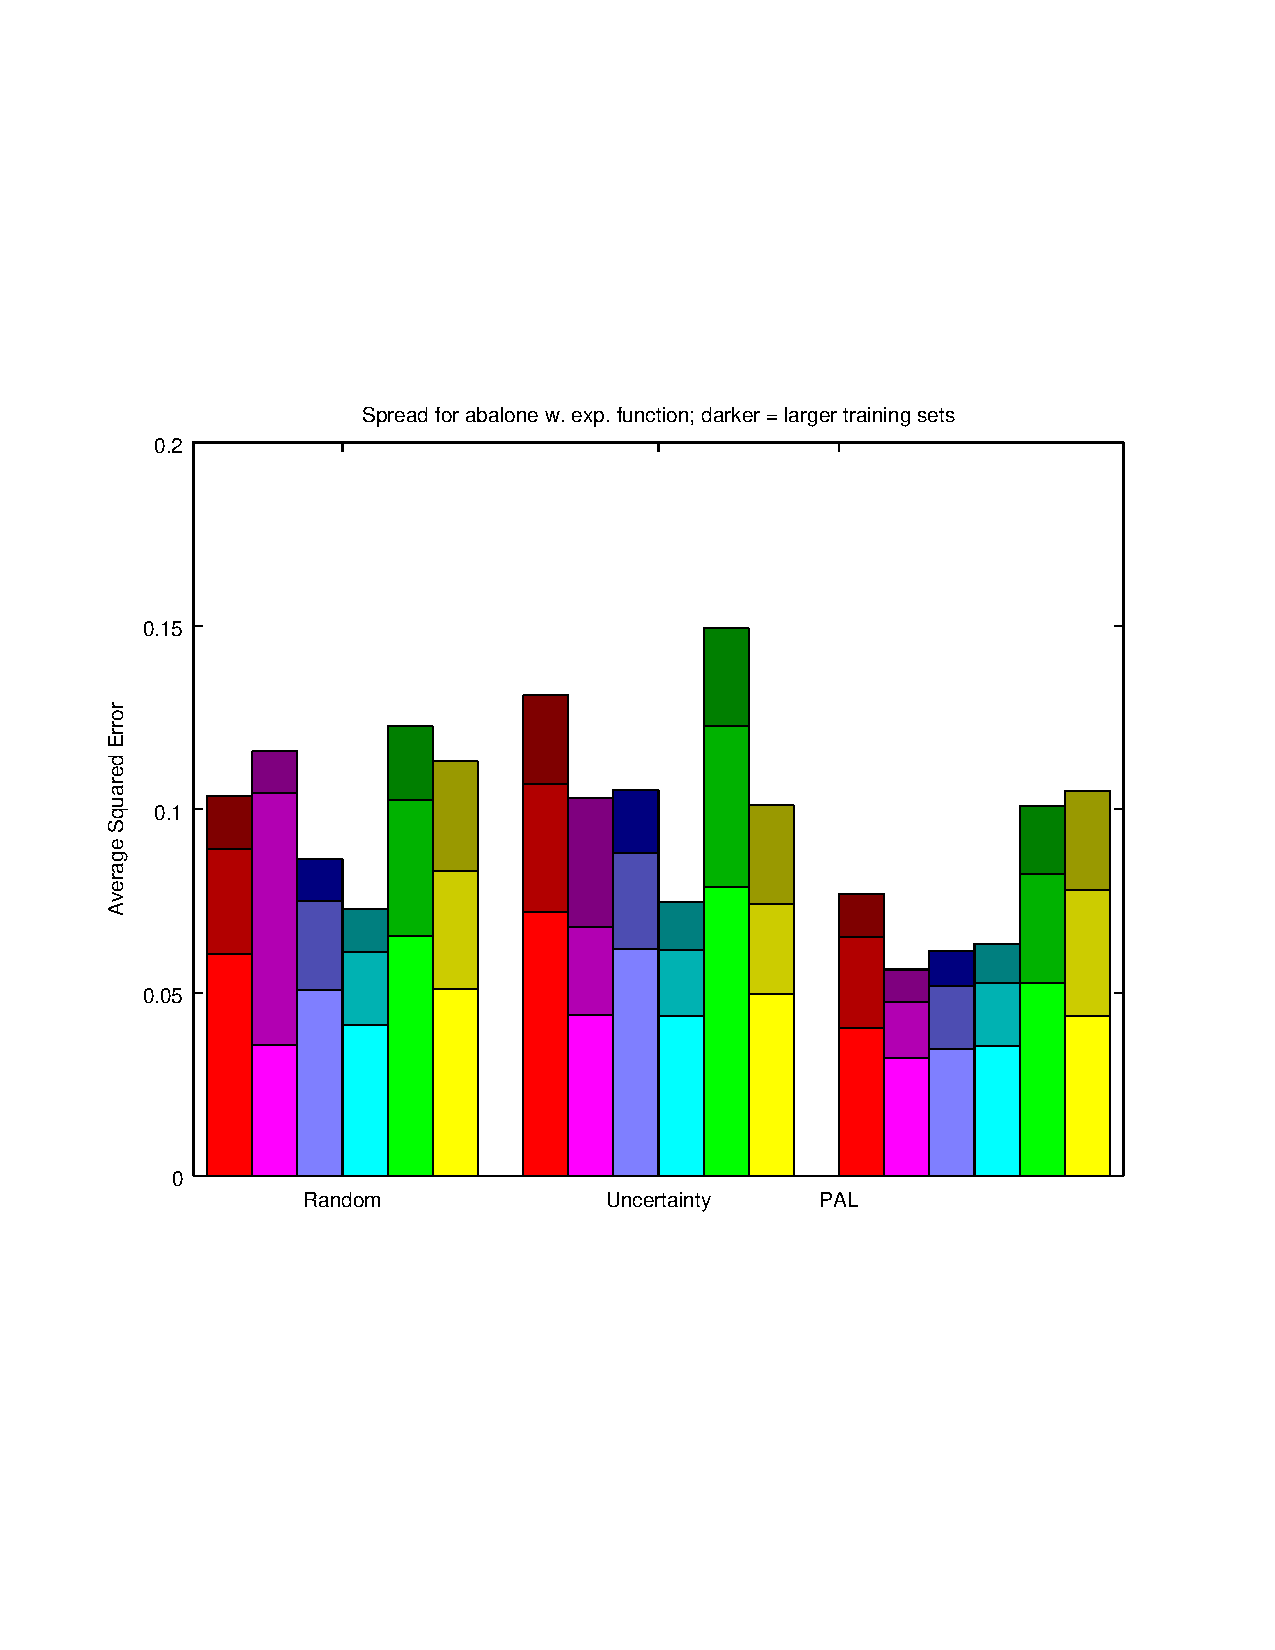
\includegraphics[trim = 0.8cm 6.5cm 2.5cm 6.5cm, clip = true, width = 0.48\textwidth]{squErrabalone}
	\caption{Average squared errors for the different active learners and datasets with the respective share of each learning stage}
	\label{fig:squaredErrors}
\end{figure}

Similarly to the estimation bias, both non-random active learners tend to come with an increase in spread. This is to be expected, as a high error implies a high squared error. For the most part, \textit{.632+ BS} has the lowest spread, while \textit{averaged}, \textit{averagedBS} and \textit{5-Fold CV} mark the upper end. With random sampling, the spread drops for larger $k$ for all estimators, as it is to be expected: more training instances mean more subsets, which increases the amount of accuracy estimates available for the model fitting. This is not the case for uncertainty sampling, as the additional estimates are obtained from more instances at a (likely) noisy decision boundary.

PAL, on the other hand, does not induce this behavior except for the special case of checke1, where the spread doubles from the early to middle learning stage and then drops again. The reason for this peak lies again in checke1's checkerboard structure. When $k \in [3,7]$, not every checker field has been covered by a purchase, fusing some of them together from the classifier's point of view. In the middle stage, every field should have at least one training instance, but not yet two. Where there was the chance that a left out instance's field was covered by an instance with equal class label because an adjacent field did not have an instance yet, this possibility is now excluded. It will only not be a misclassification if a second instance has already been purchased for the field, and even then it is not completely excluded, e.g. if both instances lie at the borders of the field. When $k \in [16,30]$, however, every field should be covered by at least two or three instances, steadily decreasing the misclassifications in estimation. And since a high bias implies a higher spread (not variance!), this explanation is valid for both.

\subsection{Kullback-Leibler divergence}

\begin{figure}[h]
	\centering
	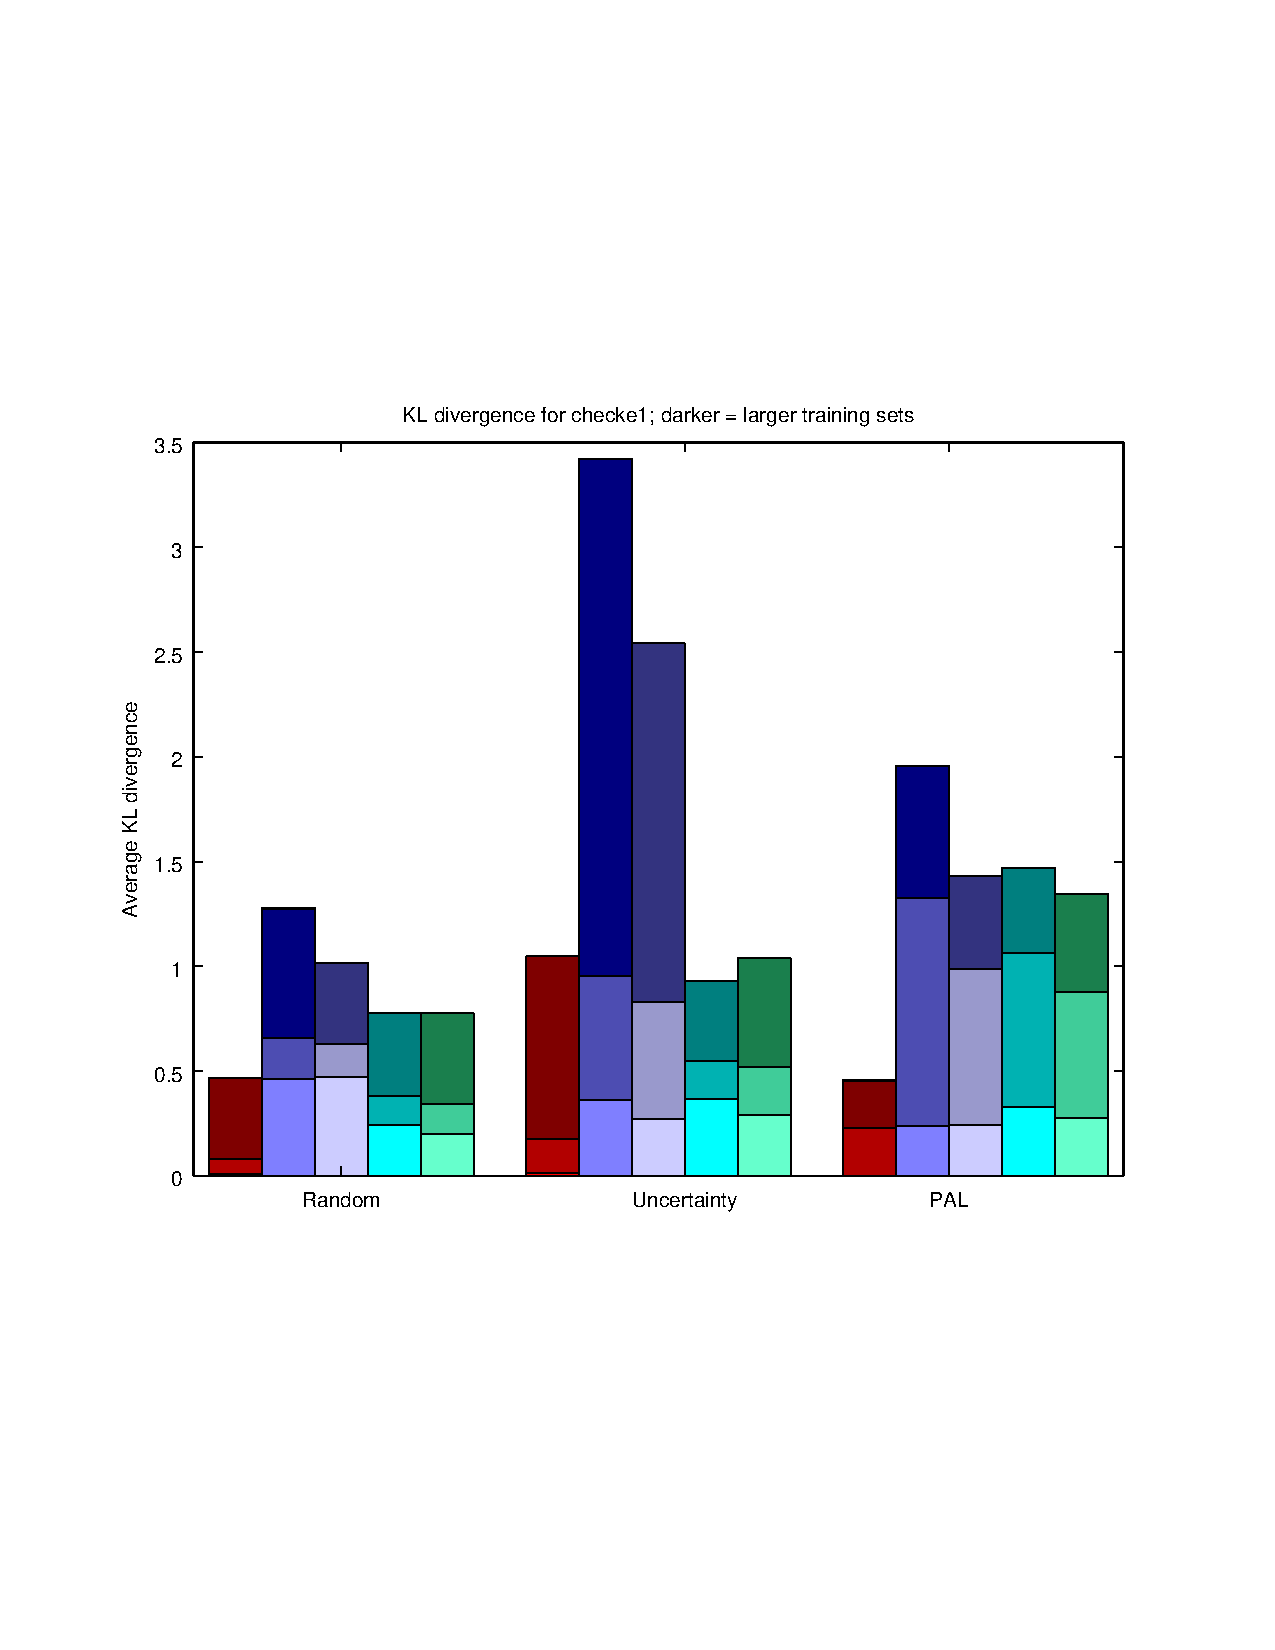
\includegraphics[trim = 1cm 7cm 2.5cm 6cm, clip = true, width = 0.48\textwidth]{klDivchecke1}
	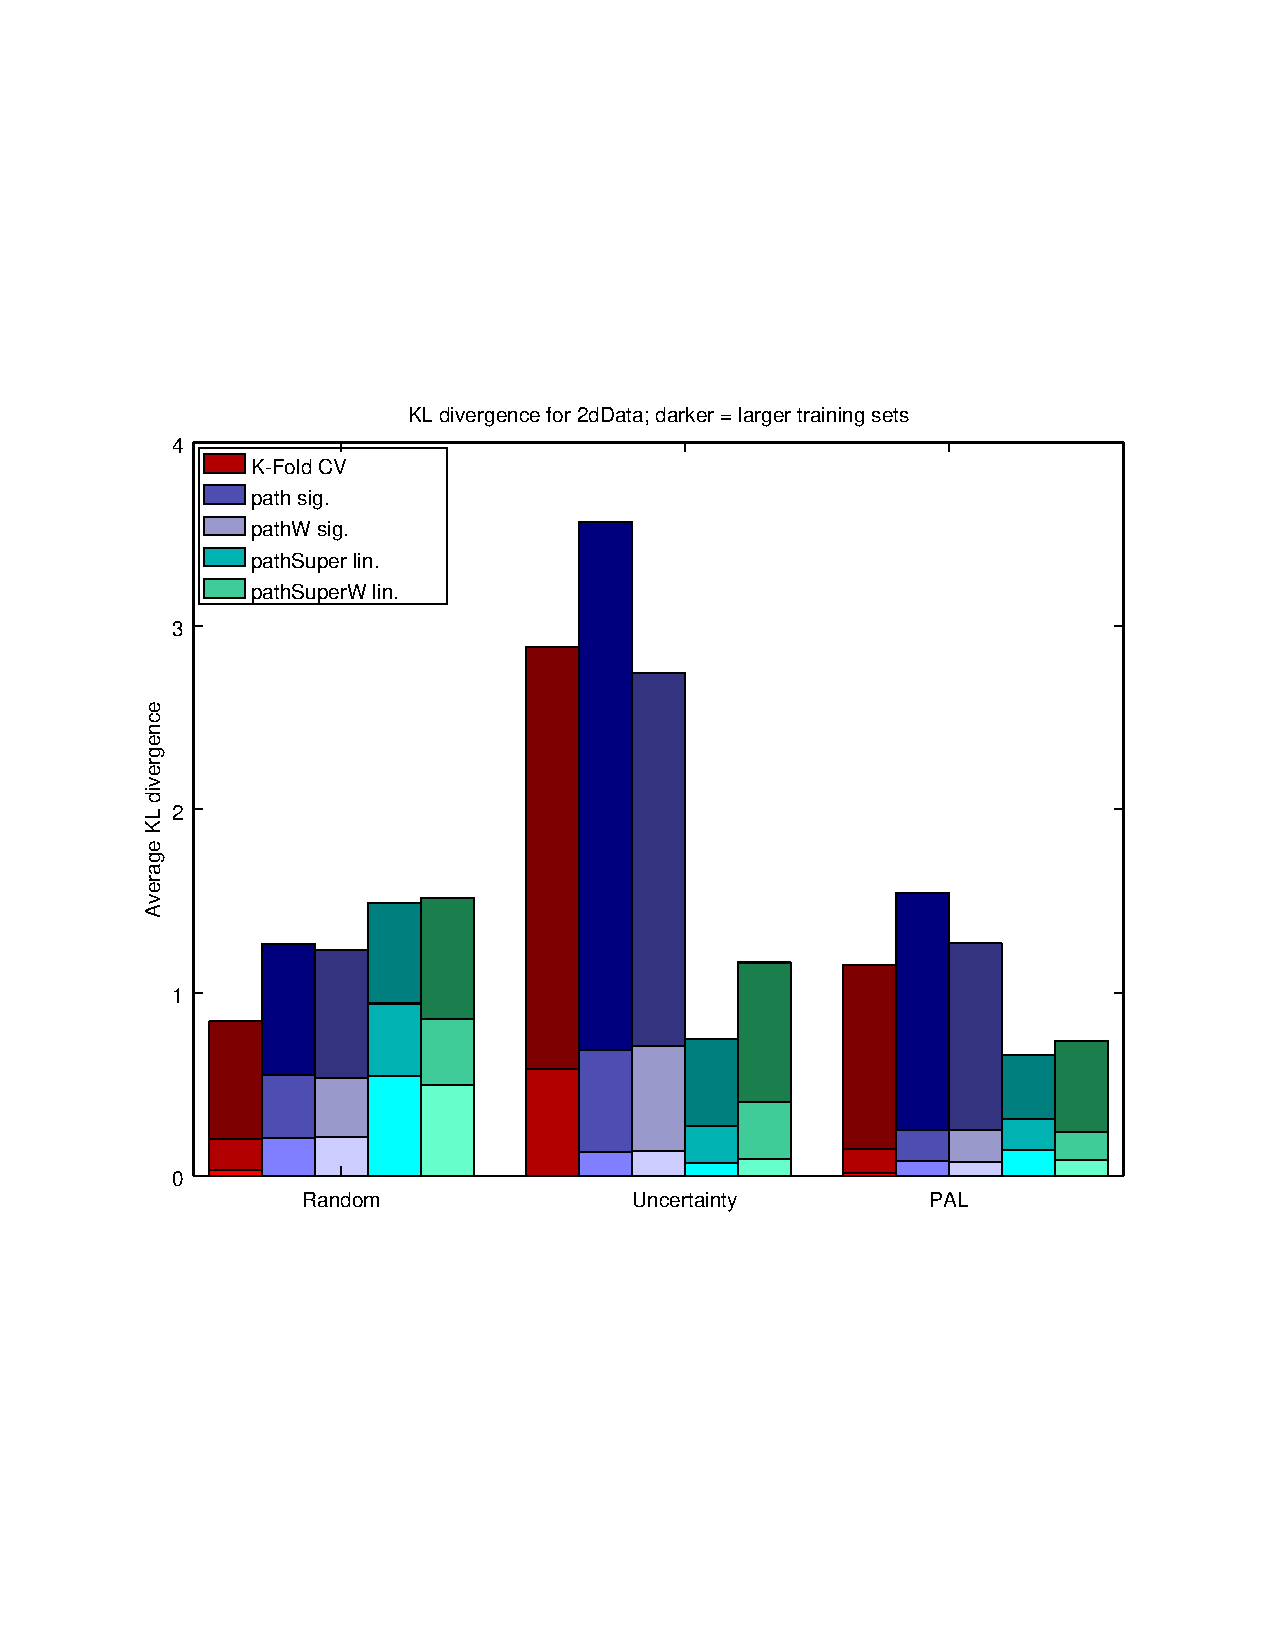
\includegraphics[trim = 1cm 7cm 2.5cm 6cm, clip = true, width = 0.48\textwidth]{klDiv2dData}
	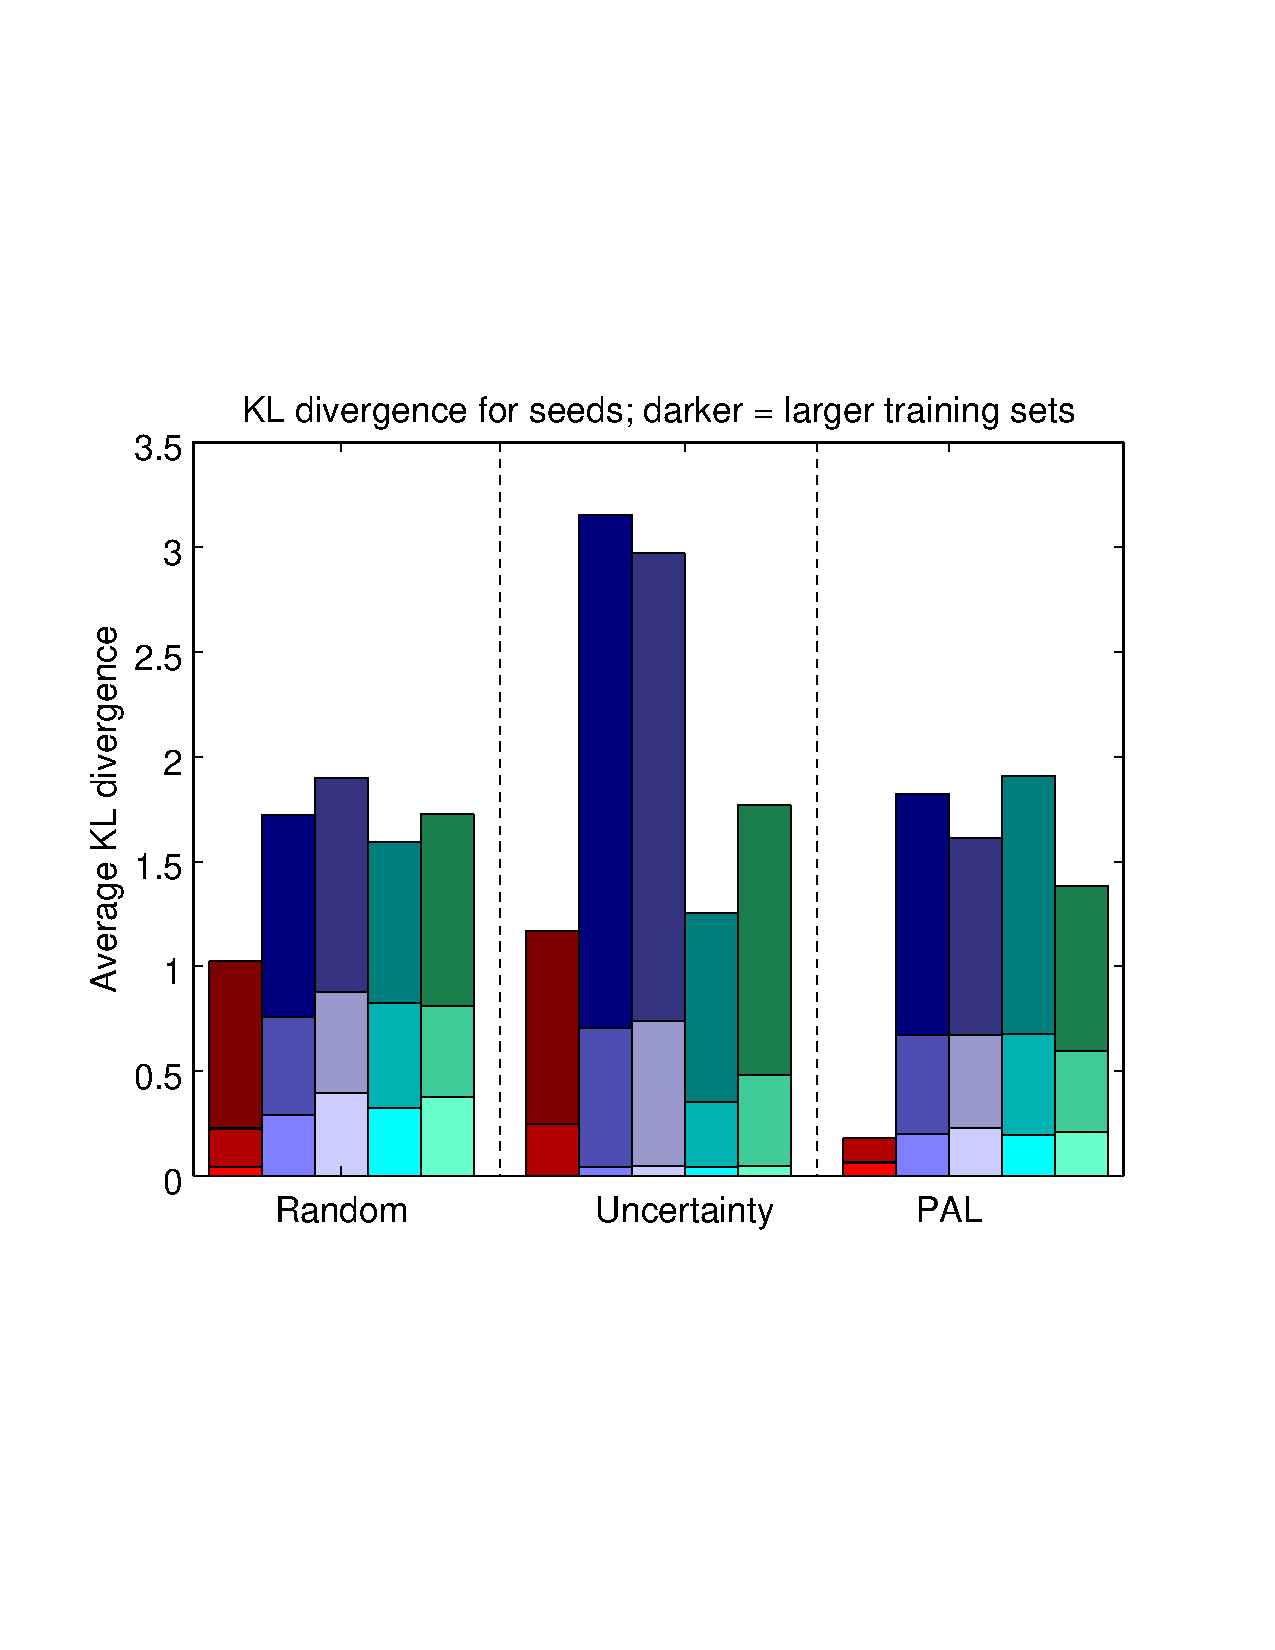
\includegraphics[trim = 1cm 7cm 2.5cm 6cm, clip = true, width = 0.48\textwidth]{klDivseeds}
	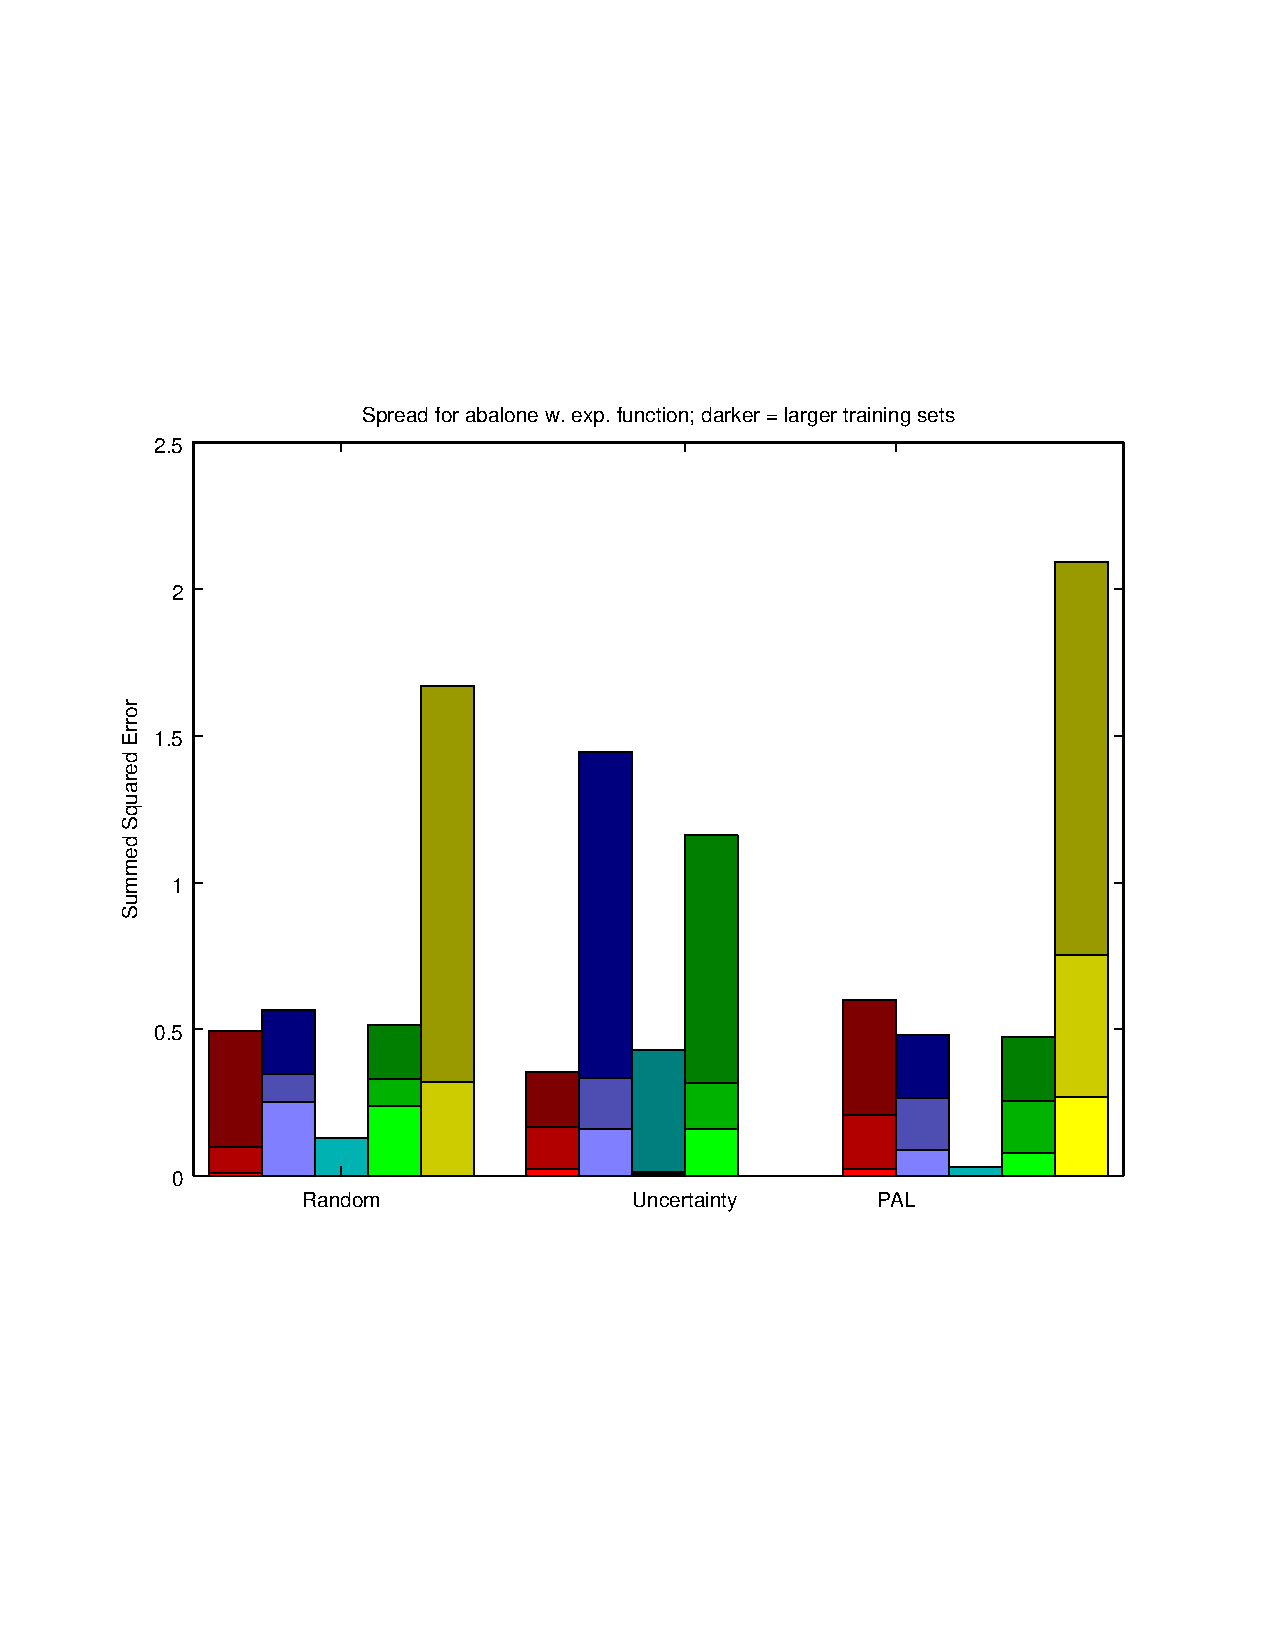
\includegraphics[trim = 1cm 7cm 2.5cm 6cm, clip = true, width = 0.48\textwidth]{klDivabalone}
	\caption{Average Kullback-Leibler divergence for selected methods}
	\label{fig:klDiv}
\end{figure}

\ref{fig:klDiv} depicts the average Kullback-Leibler divergences of selected estimators. \textit{5-Fold CV} offers the smallest divergence across the board, while neither of the \textit{path} nor the \textit{pathSuper} methods provide distributions with a lower KLD than that in a recognizable order. Surprisingly, the average divergence rises across the board for larger training sets, which is quite in contrast to the bias. However, its meaning should not be rated too high; after all, the performance estimators are meant to estimate the accuracy, which is only the mean of the accuracy's distribution, while its variance is not part of the estimation itself. Also, since it is not always possible to obtain a variance estimate, it is ill-advised to use the KLD as a primary comparison tool.

\subsection{Computation Time}

To finish the evaluation, \ref{fig:compTimeAll} shows the average computation time needed for each method with the exponential function model. As statistical weights should not alter the time too much, these variants were omitted. It shows immediately that none of the methods illustrated in \ref{methods} are anywhere near as fast as either \textit{5-Fold CV} or \textit{.632+ BS}. In fact, if all available estimates/paths were to be used, every one of these estimators would scale exponentially with the training set size. Especially expensive is the bootstrap averaging, as bootstrapping itself is more complex than cross-validation. Although it is not shown, the linear function model allows for slightly faster fitting, which could be improved more if the parameters would be computed directly instead of approximated with Levenberg-Marquardt. It also has to be said that the choice of programming language may play a big role; since it uses an interpreter, Octave usually runs slower than other high-level languages like C++, with even more penalties to its execution speed when the code is not properly vectorized.

\begin{figure}[h]
	\centering
	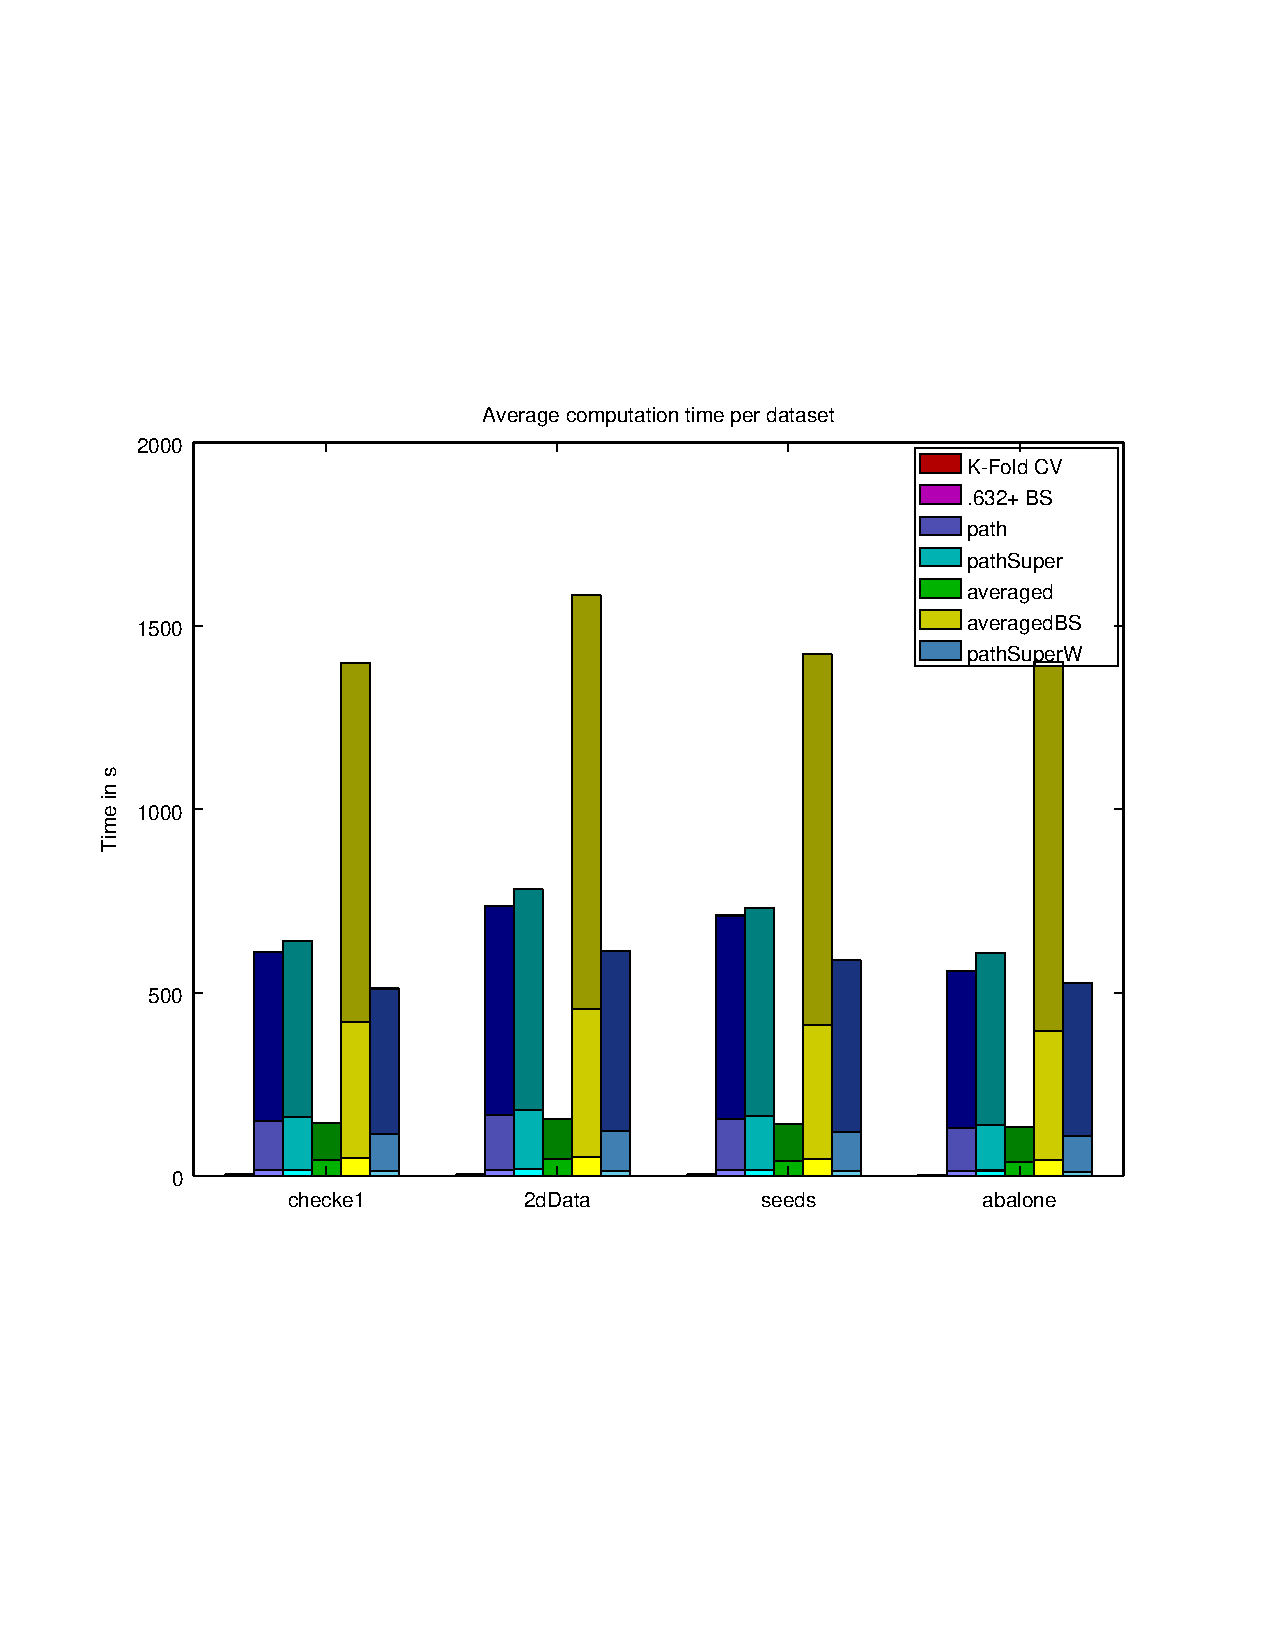
\includegraphics[trim = 1.5cm 7cm 2.5cm 6cm, clip = true, width = 0.48\textwidth]{timeAll}
	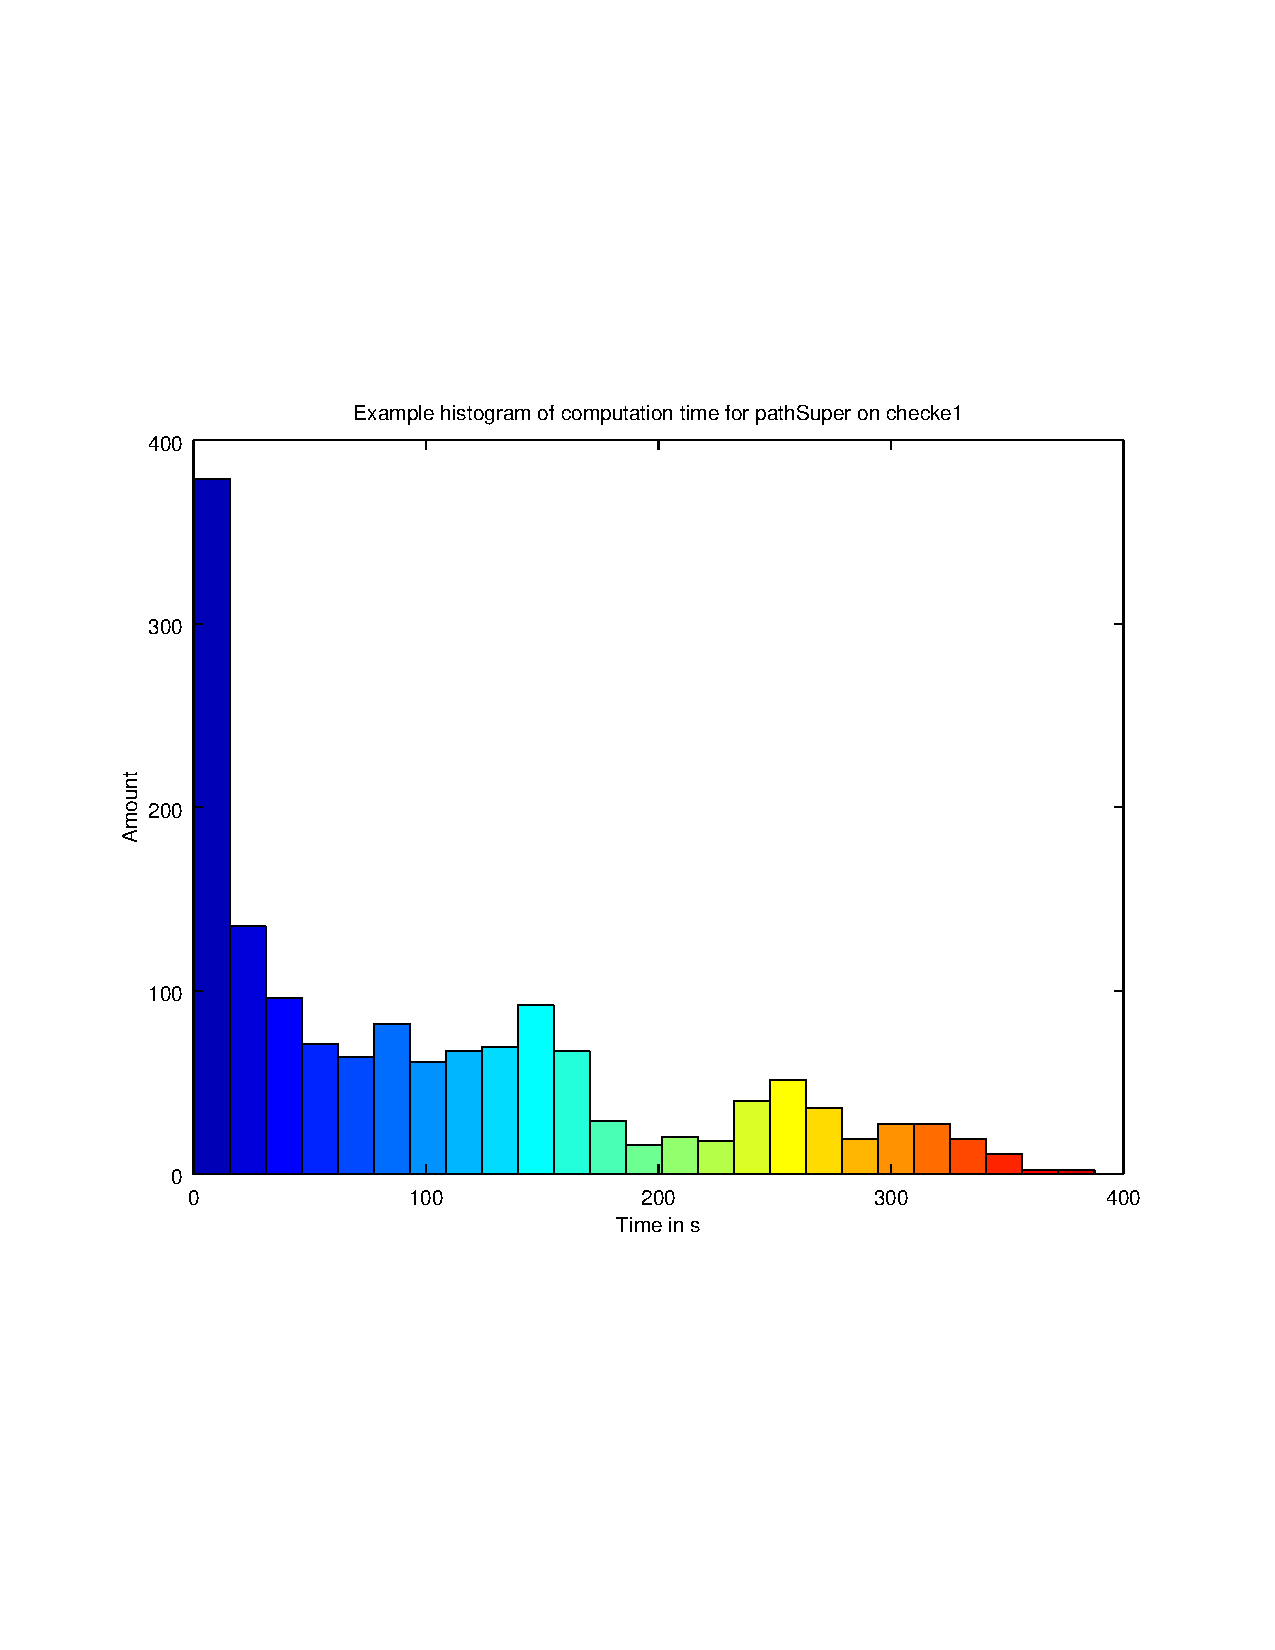
\includegraphics[trim = 1.5cm 7cm 2.5cm 6cm, clip = true, width = 0.48\textwidth]{timeHistExample}
	\caption{Left: Average computation times for the estimators. Right: Histogram of computation time for pathSuper}
	\label{fig:compTimeAll}
\end{figure}

The computation time is also independent of the used dataset and, as implicated by the absence of a distinction, the active learner, although the Parzen window classifier does scale with the data's dimensionality. However, the model fitting and subset creation take up significantly more resources. Pictured in \ref{fig:compTimeAll} is a histogram for the computation times for \textit{pathSuper} with the exponential model on checke1. Its spread is partly due to the variability in number of iterations for the fitting, but also because estimations for all training set sizes were utilized in its creation.